\documentclass[letterpaper, 12pt, oneside]{tesis}

\setlength\paperheight{11in}
\setlength\paperwidth{8.5in}

\usepackage[spanish]{babel}
\selectlanguage{spanish}
\usepackage[utf8]{inputenc}
\usepackage[fixlanguage]{babelbib}
\usepackage[T1]{fontenc}
\usepackage{natbib}
\usepackage{enumerate}
\usepackage{tikz}
\usepackage{color}
\usepackage{xcolor,colortbl}
\usepackage{verbatim}
\usepackage{fancyvrb}
\usepackage{hyperref}
\hypersetup{urlcolor=blue, colorlinks=false}
\usepackage{mathrsfs,amsmath}
\usepackage{amsthm}
\usepackage{amssymb}
\usepackage{mdframed}
\usepackage{blindtext}
\usepackage{paralist}
\usepackage{parskip}
\usepackage{multirow}
\usepackage[noend]{algpseudocode}
\usepackage[chapter]{algorithm}
\usepackage{titlesec}
\usepackage{adjustbox}
\usepackage{graphicx}

\titleformat{\chapter}[display]
{\normalfont\huge\bfseries}{\chaptertitlename\ \thechapter}{0pt}{\Huge}
\titlespacing*{\chapter}{0pt}{1cm}{40pt}

\floatname{algorithm}{Algoritmo}
\renewcommand{\algorithmicrequire}{\textbf{Input:}}
\renewcommand{\algorithmicensure}{\textbf{Output:}}
\renewcommand{\algorithmiccomment}[1]{\hfill \tiny//~#1\normalsize}
\decimalpoint

\setcounter{secnumdepth}{4}
\titleformat{\paragraph}
{\normalfont\normalsize\bfseries}{\theparagraph}{1em}{}
\titlespacing*{\paragraph}
{0pt}{3.25ex plus 1ex minus .2ex}{1.5ex plus .2ex}

\let\oldtabular\tabular
\renewcommand{\tabular}{\footnotesize\oldtabular}

\graphicspath{{img/}}

% Sangrías de 3 espacios (3 veces el espacio de la x)
\parindent 3ex 
% Interlineado
\setlength{\baselineskip}{1.5pt}
% Interpárrafo
%\setlength{\parskip}{16.5pt}

\topmargin 2cm

\renewcommand\spanishtablename{Tabla}
\renewcommand{\arraystretch}{1.1}
\definecolor{Gray}{gray}{0.95}
\newcolumntype{g}{>{\columncolor{Gray}}c}

\newcommand\listsymbolname{Acrónimos y Símbolos}

% Definiciones
%\theoremstyle{plain}
%\newtheorem{thm}{Theorem}[section]

\theoremstyle{definition}
\newtheorem{definicion}{Definición}

% Portada
\begin{titlepage}
    \title{\vspace{-2cm} 
\includegraphics[width=1.2in]{./usb.pdf} \\[.2cm]
        \large Universidad Simón Bolívar \\
        Decanato de Estudios Profesionales \\
        Coordinación de Ingeniería de la Computación
        \vfill \LARGE Selección de prototipos: un estudio experimental \vfill}
    \author{Por: \\
        Antonio Álvarez \\[1.2cm]
        Realizado con la asesoría de: \\
        Emely Arráiz B.\\[1.2cm]
        PROYECTO DE GRADO \\
Presentado ante la Ilustre Universidad Simón Bolívar \\
como requisito parcial para optar al título de \\
Ingeniero de Computación}
    \date{Sartenejas, diciembre de 2018}
\end{titlepage}

\begin{document}
\frontmatter
\maketitle
\setstretch{1.3}

% +------+
% | ACTA |
% +------+
%\begin{minipage}[height=11in]{8.5in}
%\vspace*{-2.8cm}
%\hspace*{-3.5cm}
%\includegraphics[width=8.5in]{acta}
%\end{minipage}

% +---------+
% | RESUMEN |
% +---------+
\newpage
\addtotoc{Resumen}
\abstract{
\addtocontents{toc}{\vspace{1em}}

El continuo crecimiento en la cantidad de información almacenada en bases de datos, producto de los avances en la academia y en la industria, ha traido problemas de escalamiento en la aplicación de algoritmos de minería de datos. Es por eso que se necesita adoptar un método de reducción de datos que sea eficaz y eficiente, es aquí donde tiene relevancia el problema de Selección de Prototipos (PS por sus siglas en inglés), el cual consiste en seleccionar el subconjunto de instancias de menor cardinalidad apartir de un conjunto base, que mantenga o mejore la precisión de clasificación al ser usado como conjunto de entrenamiento \cite{garcia2016data}. Como las metaheurísticas (algoritmos de proposito general enfocados a conseguir ``buenas'' soluciones a un problema determinado) son las candidatas para resolver PS, en este trabajo se busca evaluar si al darles información procesada y filtrada previamente por otros métodos, se puede mejorar el desempeño de las mismas. Para lograr este cometido, se combinan tres metodos de filtrado prevido (CNN, ENN y RSS) con cuatro metaheurísticas (GGA, SSGA, MA y CHC) y se evalúan con respecto a la precisión en la clasificación y la tasa de reducción de instancias. La evaluación experimental indica que GGA y SSGA fueron beneficiadas por el uso de un filtro previo (en este caso, el uso de CNN y RSS), mientras que MA y CHC no. Por otra parte, la versión original de CHC obtiene los mejores resultados, entre las 4 metaheurísticas estudiadas, bajo las métricas utilizadas. 

}

% Las palabras clave son generalmente los nombres de áreas de investigación a
% los cuales está asociado el trabajo. Generalmente son tres o cuatro.
\noindent \begin{small} \textbf{Palabras clave}: reducción de datos, selección de prototipos, heurísticas, metaheurísticas.
\end{small}


\clearpage
\setstretch{1.3}

% +-----------------+
% | AGRADECIMIENTOS |
% +-----------------+
%\acknowledgements{
\addtocontents{toc}{\vspace{1em}}

\blindtext

}
\clearpage


%\pagestyle{fancy}

% +--------+
% | INDICE |
% +--------+
\lhead{\emph{Índice General}}
\tableofcontents

\lhead{\emph{Índice de Figuras}}
\listoffigures

\lhead{\emph{Índice de Tablas}}
\renewcommand*\listtablename{Índice de Tablas}
\listoftables

\lhead{\emph{Índice de Algoritmos}}
\renewcommand*\listalgorithmname{Índice de algoritmos}
\listofalgorithms
\addcontentsline{toc}{chapter}{Índice de algoritmos}

% +----------------------+
% | ACRONIMOS Y SIMBOLOS |
% +----------------------+
\setstretch{1.5}
\clearpage
\lhead{\emph{Acrónimos y símbolos}}
\listofsymbols{ll}
{

    % Aquí van las siglas
    \textbf{KDD}  & Knowledge Discovery in Databases\\
    \textbf{DM}   & Data Mining\\
	\textbf{IS}   & Instance Selection\\
	\textbf{PS}   & Prototype Selection\\
	\textbf{NN}   & Nearest Neighbor\\
	\textbf{NE}   & Nearest Enemy\\
	\textbf{CNN}  & Condensed Nearest Neighbor\\
	\textbf{ENN}  & Edited Nearest Neighbor\\
	\textbf{RSS}  & Relaxed Selective Subset\\
	\textbf{GGA}  & Generational Genetic Algorithm\\
	\textbf{SGA}  & Steady-State Genetic Algorithm\\
	\textbf{CHC}  & CHC Adaptive Search Algorithm\\
	\textbf{MEM}  & Memetic Algorithm\\
    &\\
    \hline
    &\\

    % Aquí van los símbolos
    $\in$ & Relación de pertenencia, \guillemotleft\emph{es un elemento de}\guillemotright\\
	$\subseteq$ & Subconjunto\\
	$\setminus$ & Diferencia de conjuntos
}

\setstretch{1.3}


\pagestyle{empty}

% +-------------+
% | DEDICATORIA |
% +-------------+
%\dedicatory{
    \textbf{Dedicatoria} \bigskip

    A @personasImportantes, por @razonesDedicatoria.
}

\addtocontents{toc}{\vspace{2em}}


\mainmatter
\pagestyle{fancy}

% +--------------+
% | INTRODUCCION |
% +--------------+

\chapter*{Introducción}
\label{intro}
\lhead{\emph{Introducción}}
\addcontentsline{toc}{chapter}{Introducción}

Introdución


% +-----------+
% | CAPITULOS |
% +-----------+
\chapter{Marco teórico}
\label{capitulo1}
\lhead{Capítulo 1. \emph{Marco teórico}}

\section{Descubrimiento de Conocimiento y preprocesamiento de datos}

Hoy en día, existe una creciente necesidad de procesar grandes volúmenes de datos, estos datos son producto de la recolección de información de procesos y actividades de distintas índoles y se vuelven un material valioso para extraer información sobre posibles tendencias que puedan existir en dichos procesos. Es aquí donde entra el descubrimiento de conocimiento en bases de datos (KDD por su ssiglas en inglés) como disciplina encargada del procesamiento de datos para la extracción de información.

KDD es definida por Smyth, P. et al. \cite{fayyd1996data} como ``el proceso no trivial de identificar patrones en los datos que sean válidos, novedosos, potencialmente útiles y finalmente entendibles''. Para este fin, KDD se subdivide en distintas etapas a llevar a cabo para lograr el fin último de identificar patrones, éstas son \cite{garcia2016data}: especificación del problema, entendimiento del problema, preprocesamiento de los datos, minería de datos, evaluación de los resultados y explotación de los resultados. En este trabajo es de especial interés la etapa de preprocesamiento de datos.

El preprocesamiento de datos consiste en el conjunto actividades destinadas a preparar los datos para ser usado por un algoritmo de minería de datos. Las actividades realizadas en el preprocesamiento pueden ser clasificadas como actividades para la preparación de los datos y la reducción de los mismos \cite{garcia2016data}.

La preparación de datos es un paso obligatorio en el preprocesamiento ya que transforma los datos, que inicialmente son inservibles para el algoritmo de DM por asuntos como la presencia de atributos faltantes en instancias, datos erróneos y atributos con formatos no aceptables para el algoritmo a utilizar \cite{garcia2016data}. Dependiendo del enfoque dado, estas actividades pueden clasificarse en:

\begin{itemize}
\item \textbf{Limpieza de datos \cite{garcia2016data, kim2003taxonomy}}
Incluye el tratamiento de los atributos faltantes y los datos erróneos, que si se dejan sin tratar resulta en un modelo de minería de datos poco confiable. Un atributo faltante en una instancia resulta de no haberlo introducido al momento del registro o por la pérdida en el proceso de almacenamiento. Los datos con atributos faltantes pueden tratarse de 3 maneras \cite{farhangfar2007novel}: la eliminación de las instancias que presenten el problema, utilizar métodos de estimación de máxima verosimilitud para calcular promedios y variancias con lo cual llenar los atributos faltantes y utilizar algoritmos del repertorio de machine learning como k-nn, k-means o Suport Vector Machine para estimar el valor de los atributos faltantes. 

Por su parte, los datos erróneos (también conocidos como datos ruidosos) pueden venir de dos formas \cite{catal2011class}: ruido de clase cuando la instancia está mal clasificada y ruido de atributo cuando uno o más valores de atributos en una instancia están distorisionados y no representan la realidad. Para tratar los datos ruidosos se puede usar 3 métodos: construir algoritmos de minería de datos que no se vean afectados en cierta medida ante el ruido (sean robustos), pulir los datos \cite{teng1999correcting} de tal manera que se corrijan los errores y por último se puede identificar los datos ruidosos para eliminarlos del conjunto y así quedarse sólo con datos correctos \cite{brodley1999identifying}. Cada uno de estos métodos tiene sus ventajas y desventajas; si sólo se cuenta con lo robusto del algoritmo de clasificación o regresión se tiene que tendrá un nivel de tolerancia del cual al pasarse los resultados serán inservibles, pulir los datos sólo es aplicable a conjuntos de tamño pequeño y mediano debido al alto costo computacional que tienden a tener los algoritmos que hacen el trabajo y si se decide filtrar todos los datos ruidosos se puede disminuir considerablemente el conjunto hasta un punto que no sea utilizable por los algoritmos de clasificación y regresión; por lo tanto, lo que se estila es usar una combinación en lo que sea posible de estos 3 métodos para obtener los mejores resultados

\item \textbf{Transformación de datos \cite{garcia2016data}}
Se centra en aplicar fórmulas matemáticas a los valores de los atributos para así obtener valores sintéticos que pueden proporcionar más información respecto a la instancia y al conjunto que pertenencen. Las transformaciones más comunes son la lineal y la cuadrática, la primera se usa principalmente para combinar distintos atributos y así crear uno sintético para ser usado por el algoritmo de minería de datos, la transformación cuadrática por su parte, es usada cuando una transformación lineal no es suficiente para derivar información útil de los atributos. En este sentido, existen otros tipos de transformaciones como la polinomial que engloba a la lineal y a la cuadrática y la no polinomial que trata con transformaciones más complejas.

\item \textbf{Integración de los datos \cite{garcia2016data,batini1986comparative}}
Consiste en la unión de las conjuntos de datos provenientes de distintas fuentes en un único conjunto. La integración tiene que tomar en cuenta algunos aspectos que se pueden presentar durante el proceso, entre ellos están la redundacia de atributos, la cual sucede cuando 2 atributos están fuertemente correlacionados y por lo tanto, con tener uno de ellos se puede derivar el otro. La redundancia de atributos puede traer consigo un sobre ajuste (overfitting) de los modelos predictivos, además de aumentar el tiempo de cómputo de los mismos, es por eso que se debe eliminar esta redundancia y para ello se usa una prueba de correlación $\chi^2$ con el fin de identificar los atributos redundantes y así decidir con cual quedarse. 

Continuando, con los problemas que se pueden presentar al momento de la integración, se tiene también la duplicación de instancias. Problema que normalmente trae consigo la inconsistencia en los valores de los atributos debido a las diferencias con las que se registran los valores. Para solucionar este problema primero se tiene que identificar las instancias duplicadas usando técnicas de identificicación de similitud como la propuesta de \emph{Fellegi y Sunter} \cite{fellegi1969theory} que lo modela como un problema de inferencia bayesiana o como en \cite{cochinwala2001efficient} donde se usan árboles de clasificación y regresión (CART por sus siglas en inglés) para cumplir este trabajo.

\item \textbf{Normalización de datos \cite{garcia2016data}}
Busca cambiar la distribución de los datos originales de tal manera que se acoplen a las necesidades de los algoritmos predictivos. Dos de los tipos de normalización más usadas son la normalización min-max en la cual se aplica la fórmula en la ecuación 1.1, donde $max_A$ es el valor máximo del atributo sobre los valores en el conjunto, $min_A$ es el valor mínimo existente, $nuevo\_max_A$ y $nuevo\_min_A$ son los nuevos rangos para el atributo:

\begin{equation}
v' = \frac{v-min_A}{max_A-min_A}(nuevo\_max_A - nuevo\_min_A) + nuevo\_min_A
\end{equation}

El otro tipo de normalización es la puntuación Z (Z-score) en donde se llevan los datos a promedio 0 y desviación estándar 1 aplicando la fórmula de la ecuación 1.2:

\begin{equation}
v' = \frac{v-\mu_A}{\sigma_A}
\end{equation}
.\end{itemize}

Pasando a la reducción de los datos, se tiene que engloba todas las técnicas que reducen el conjunto de datos original para obtener uno representativo con el cual trabajar en los modelos predictivos. La reducción de datos cobra especial importancia cuando se tienen conjuntos muy grandes que retardarían en gran medida el tiempo de cómputo de los algorimtos que los van a usar. Las técnicas de reducción de datos son \cite{garcia2016data}:

\begin{itemize}
\item \textbf{Discretización de datos \cite{garcia2016data,garcia2013survey}}
Es el proceso de transformar datos numéricos en datos categóricos, definiendo un número finito de intervalos que representan rangos entre distintos valores consecutivos con el fin de poder tratarlos como valores nominales. Es de especial importancia el conseguir el número correcto de intervalos que mantengan la ínformación original de los datos, ya que muy pocos intervalos puede llegar a ocultar la relación existente entre un rango en específico y una clase dada y muchos intervalos puede llevar a un sobre ajuste \cite{cios2007data}. El principal atractivo de la discretización es que permite utilizar un algoritmo de minería de datos que trabaje principalmente con datos nominales como Naïve Bayes \cite{yang2009discretization} a partir de datos numéricos. Para un estudio más completo de la discretización se referencia a \cite{garcia2013survey}.

\item \textbf{Selección de características \cite{garcia2016data,liu2012feature}}
Busca eliminar atributos que sean redundantes o irrelevantes de tal manera que el subconjunto de características restantes mantenga la distribución original de las clases. El proceso de selección de características tiene ventajas como mantener e incluso mejorar la precisión de los modelos predictivos, reducir los tiempos de cómputo y reducir la complejidad de los modelos resultantes. La búsqueda de un subconjunto de atributos puede realizarse de 3 maneras: búsqueda exhaustiva, búsqueda heurística y métodos no determinísticos. La búsqueda exhaustiva cubre todo el espacio de soluciones, normalmente van probando todas las combinaciones posibles de atributos para conseguir el que mejor se acople a la métrica a optimizar, entre los métodos exhaustivos están Focus \cite{almuallim1991learning}, Automatic Branch \& Bound \cite{liul1998monotonic}, Best First Search \cite{xu1988best}, entre otros. Por su parte, la busqueda heurística busca una solución aproximada a la óptima en poco tiempo, entre sus métodos están los propuestos en \cite{dash1997feature,koller1996toward,battiti1994using}. Por último, están los métodos no determinísticos, de entre los que destacan los algoritmos géneticos, recocido simulado y Las Vegas Filter \cite{liu1996probabilistic}.

\item \textbf{Selección de instancias \cite{garcia2016data}}
Consiste en elegir un subconjunto de las instancias totales manteniendo las características del conjunto original. Es el problema a tratar en este trabajo y se elabora más sobre el mismo en la siguiente sección.
\end{itemize}

\section{Selección de Instancias y Selección de Prototipos}

La selección de instancias (IS por sus siglas en inglés) consiste en reducir el conjunto de datos dado a un conjunto reducido que va a ser utilizado con un algoritmo clasificador, manteniendo el desempeño del algorimto como si se usara el conjunto original.\\

\begin{definicion}
Dado un conjunto de datos X, se tiene que una instancia $X_i = (X_i^1,X_i^2,\dots,X_i^p)$ donde $X_i^j$ es el atributo j para la instancia $X_i$ con $X_i\in X$ y siendo p el número de atributos. La instancia $X_i$ es de clase $Y_j$ donde $Y_i\in Y$, siendo Y el conjunto de todas las clases definidas con $j\in (1\dots q)$ donde q es el número de clases totales. Se divide el conjunto X en un conjunto TR de entrenamiento y un conjunto TS de prueba. El problema de \textbf{Selección de Instancias} consiste en conseguir un conjunto ${S\subset TR$ con el cual al usarse con el clasificador T se obtengan los mismos valores de precisión o mejores que al usar T con TR \cite{garcia2016data}.
\end{definicion}

La respuesta óptima de un método de selección de instancias es un conjunto \emph{consistente} y de cardinalidad mínima.\\

\begin{definicion}
``Un conjunto $R$ es \textbf{consistente} con $T$, \emph{si y solo si} toda instancia $t \in T$ es clasificada correctamente mediante el uso de un clasificador \emph{M} y las instancias en $R$ como conjunto de entrenamiento.'' \cite{flores2014metaheuristics}
\end{definicion}

Sin embargo, conseguir la respuesta óptima es un problema NP-Duro (NP-Hard) como lo demuestra \emph{Zukhba} en \cite{zukhba2010np}. Por lo tanto, la mayoría de los métodos propuestos hasta la fecha se enfocan en obtener una solución aproximada.

El problema de selección de instancias se puede enfocar como un problema de selección de prototipos (PS por sus siglas en inglés). PS es en esencia IS con el detalle de que el clasificador T usado es un clasificador basado en instancias \cite{garcia2016data}. De los cuales K Vecinos más Cercanos (KNN por sus siglas en inglés) es el más conocido y el cual será usado como clasificador para este trabajo.

\subsection{K Vecinos más Cercanos (KNN)}


\chapter{Marco metodológico}
\label{capitulo2}
\lhead{Capítulo 2. \emph{Marco metodológico}}

En este capítulo se detalla la representación utilizada para los cromosomas, la función objetivo, las adaptaciones particulares que se hizo a cada algoritmo evolutivo usado en el experimento, el proceso de validación cruzada, la técnica de estratificación, se presenta los conjuntos de datos usados para el experimento y se explica el método de entonación utilizado para ajustar los algoritmos evolutivos.

\section{Representación del cromosoma}

Sea T el conjunto de instancias a reducir de tamaño \texttt{n}, la representación usada para modelar el problema de selección de prototipos es el de un mapa de bits de tamaño \texttt{n}, donde cada bit representa una instancia dentro de T; si el valor del bit i es 1, entonces la instancia $t_i \in T$ está en el conjunto reducido S, si el bit i es 0, $t_i$ se encuentra por fuera de S. En este sentido, el conjunto $S_M$, que representa el conjunto reducido S dado por el mapa de bits M (que se le conoce también como cromosoma M y a los bits se le conoce como genes), se define como en la ecuación (2.1). Además un ejemplo se presenta en \ref{representacion}.

\begin{equation}
S_m = \left\{ t_i \in T \mid i = 1 \dots n \land s_i = 1 \right\}
\end{equation} 

\begin{figure}[]
\centering
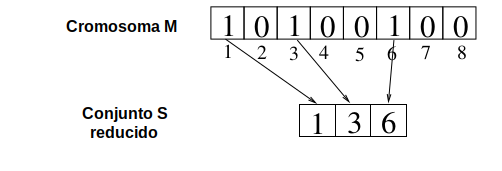
\includegraphics[height=3cm,width=10cm]{representacion.png}
\caption[Representación de un cromosoma y su respectivo conjunto reducido]{Representación de un cromosoma y su respectivo conjunto reducido}
\label{representacion}
\end{figure}

\section{Función objetivo}

Se necesita una función con la cual los algoritmos evolutivos puedan evaluar cuán buena es una solución dada, además de que dicha función debe permitir establecer una relación de orden entre las soluciones con el fin de decidir cuál cromosoma es mejor que otro. Como se explicó anteriormente, los algoritmos evolutivos buscan aproximarse al óptimo global, que en este caso es el conjunto reducido S con menor cardinalidad posible y mayor precisión en la clasificación de instancias nuevas. Es por eso que se adopta una función objetivo derivada del trabajo de \emph{Cano, J.} en \cite{de2004reduccion}, la cual se presenta a continuación:

\begin{equation}
\mathcal{F}(S) = \alpha * error(S) + (1 - \alpha) * \left( 100 * \frac{\mid S \mid}{TR} \right)
\end{equation} 

Donde $\mathcal{F}: W \rightarrow \mathbb{R}$ es la función objetivo, S es el conjunto reducido a evaluar, W es el espacio de cromosomas asociados a los distintas posibilidades de conjuntos reducidos, $\alpha$ es un parámetro que controla cuánta importancia se le da al error asociado a S con respecto a la tasa de reducción del segundo término de la ecuación (2.2), TR es el conjunto de entrenamiento original del cual se realizó la reducción y error(S) es el porcentaje de error al clasificar un conjunto de prueba TS usando 1-KNN con S como conjunto de referencia. El $\alpha$ usado es 0.5 como lo establecen en \cite{de2004reduccion} para darle la misma importancia a la reducción de datos como a mantener bajo los porcentajes de error en la clasificación.

Dado esta función objetivo, la meta de todas las metaheurísticas implementadas se vuelve minimizar $\mathcal{F}(S)$, lo cual quiere decir que se busca tanto reducir $\mid S \mid$, como reducir error(S). Una conjunto $S_i$ es mejor que un conjunto $S_j$ si $\mathcal{F}(S_i) < \mathcal{F}(S_j)$.  

\section{Adaptaciones de los algoritmos evolutivos}

Para aplicar los distintos algoritmos evolutivos implementados para este trabajo, es necesario determinar los operadores de cruce y mutación, el método de selección de los cromosomas que van a cruzarse, el criterio de selección de los cromosomas sobrevivientes y en caso del algoritmo memético el meme interno utilizado.

Para el caso del algoritmo genético estacionario y el algoritmo memético, se eligió como método se selección de cromosomas a cruzarse un proceso de torneo \cite{talbi2009metaheuristics}, el cual consiste en elegir k cromosomas de manera aleatoria y se eliminan k-1 donde el sobreviviente es el mejor dentro de los k. CHC por su parte elige dos cromosomas aleatorios y utiliza su mecanismo de prevención de incesto para elegir a los padres. El algoritmo genético generacional simplemente elige dos elementos aleatorios para realizar el cruce dada una probabilidad.

El operador de cruce utilizado en GGA, SSGA y MA es la recombinación de un punto \cite{talbi2009metaheuristics}, el cual consiste en definir un punto u en el cual se va dividir los dos cromosomas seleccionados como padres $x_1$ y $x_2$, luego se forman dos hijos $y_1$ y $y_2$ donde la mitad de sus genes provienen de de un padre y la otra mitad del otro padre. CHC en cambio usa el operador HUX explicado anteriormente. En la figura \ref{cruce} se muestra un ejemplo del cruce de un punto. 

\begin{figure}[]
\centering
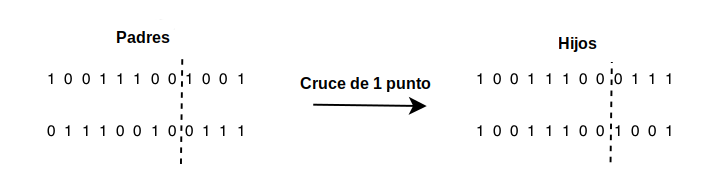
\includegraphics[width=\textwidth]{cruce.png}
\caption[Cruce de un punto]{Cruce de un punto}
\label{cruce}
\end{figure}

El operador de mutación para GGA, SSGA y MA consta de cambiar 5\% de los genes del cromosoma de manera aleatoria. Se elige 5\%  basado en \cite{flores2014metaheuristics} para que la mutación represente un cambio real en el conjunto que representa el cromosoma, ya que si sólo se cambia un gen, el conjunto mutado sería para los efectos de la optimización casi idéntico al original. Sin embargo la probabilidad de que un cromosoma dado mute es baja, basado principalmente en los resultados de \emph{Cano, J.} en \cite{de2004reduccion} donde obtienen mejores resultados experimentales con bajas probabilidades de mutación (menor al 1\% por cromosoma), justificándose en que con mayores valores, la búsqueda podría degenerar en una búsqueda aleatoria. CHC por su parte no tiene mutación.

El criterio de reemplazo para GGA es generar una población nueva de hijos $P_i$ que va a suplantar la generación anterior $P_{i-1}$ excepto el mejor elemento en $P_{i-1}$, el cual toma el lugar del peor elemento de $P_i$ en la nueva generación. Por su parte, el criterio de reemplazo de SSGA es que dado dos padres y los dos hijos producidos por el operador de cruce, se eligen los 2 mejores cromosomas para permanecer dentro de la población. MA, en cambio usa un criterio de reemplazo en el cual los 2 hijos suplantan a los 2 peores elementos de la población y CHC se queda con los \texttt{n} mejores cromosomas entre $P_i$ y $P_{i-1}$, ambos casos son totalmente elitistas.

El algoritmo memético es el que más adaptaciones tiene para adecuarse a PS, se usa una adaptación realizado por \emph{Cano, J. et al.} en \cite{garcia2008memetic}. Se basa en el algoritmo memético estacionario presentado anteriormente, con la peculiariadad de que para decidir si los hijos producidos en una iteración van a ser optimizados con el meme, se usa un parámetro $P_{LS}$ que se determina de la siguiente forma:

\begin{equation}
P_{LS}=
\begin{cases}
1 & \text{si } \mathcal{F}(S_{nuevo}) < \mathcal{F}(S_{peor})\\
0.0625 & \text{en caso contrario}\\
\end{cases}
\end{equation}

Donde $\mathcal{F}$ es la función objetivo, $S_{nuevo}$ es el conjunto reducido representado por uno de los cromosomas hijos y $S_{peor}$ es el conjunto reducido representado por el peor cromosoma de la población. Es así como $P_{LS}$ representa la probabilidad con la cual se va a decidir si se optimiza el cromosoma hijo; $P_{LS}$ debe ser calculado para cada hijo creado en el cruce. La idea es que si el hijo es mejor que el peor cromosoma de la población, entonces vale la pena optimizarlo; en cambio, si es peor, se le da una probabilidad de 6,25\%.

El meme usado en MA es el que se presenta en \ref{meme}. El procedimiento consiste en ir reduciendo progresivamente las instancias que se encuentran en el conjunto S, representado por el cromosoma M, sin que se pierda la precisión asociada a S. Para esto, se usa una lista U del primer vecino más cercano de cada gen en M, una lista R que contiene los genes que ya han sido puestos en 0 y que no generan una ganancia mayor al umbral de aceptación \texttt{t}, clase(i) es la clase asociada a la instancia representada por el gen i del cromosoma M, \texttt{ganancia} representa cuánto mejora (en caso de que sea positiva) o cuánto empeora (en caso de ser negativa) la solución dada por el cromosoma M luego de cambiar un gen, $fitness_M$ es el valor de evaluar la función objetivo con el cromosoma M y $fitness_{ganancia}$ se define como en la ecuación (2.4), donde L es el largo del cromosoma:

\begin{equation}
fitness_{ganancia} = \frac{\frac{ganancia}{L}*100 + \frac{100}{L}}{2}
\end{equation}  

El meme empieza a revisar los genes del cromosoma M que estén prendidos (con valor 1) y no se encuentren en la lista de revisados R en la línea 4; entonces, mientras se cumplan estas condiciones, se elige un $m_j$ que esté prendido y no esté en R, se apaga (coloca valor cero), se hace una copia de U a U', se actualiza la lista del primer vecino más cercano U tomando en cuenta que $m_j$ ya no pertenece al conjunto reducido S y por cada vecino de U que es actualizado, se actualiza la ganancia, sumando 1 si el gen i estaba mal clasificado anteriormente y con el nuevo vecino se clasifica correctamente (líneas 13 y 14) o restando 1 si el gen i estaba bien clasificado anteriormente y con el nuevo vecino se clasifica incorrectamente (líneas 11 y 12); acto seguido, se actualiza el \emph{fitness} del cromosoma M si la ganancia está por encima del umbral \texttt{t} y se limpia la lista de revisados R (líneas 15, 16 y 17) o en caso contrario, se recupera U con la copia U' y se prende de nuevo el gen $m_j$.  
 
\begin{algorithm}
\caption{Meme}
\label{meme}
\begin{algorithmic}[1]

\Require{\texttt{M} cromosoma a optimizar, \texttt{t} umbral de aceptación}
\Ensure{\texttt{M} cromosoma optimizado}

\State Sea $\texttt{M} = \left\{ m_1,m_2,\dots,m_n \right\}$ el cromosoma a optimizar 
\State $R \gets \emptyset$
\State $ U = \left\{ u_1,u_2,\dots,u_n \right\}$ la lista de vecinos asociados, donde $u_i$ es el vecino más cercano del gen i. 
\While{$(\exists m_i \in \texttt{M} \mid m_i = 1 \land i \notin R)$}
	\State elegir j aleatoriamente de \texttt{M} tal que $m_j=1 \land j \notin R$
	\State $ganancia \gets 0$
	\State $m_j \gets 0$
	\State Copiar U a U'
	\ForAll{$u_i \in U \mid u_i = j$}
		\State $u_i \gets$ nuevo vecino más cercano con el nuevo \texttt{M}
		\If{$clase(i) = clase(u'_i) \land clase(i) \neq clase(u_i)$}
			\State $ganancia \gets ganancia - 1$
		\ElsIf{$clase(i) \neq clase(u'_i) \land clase(i) = clase(u_i)$}
			\State $ganancia \gets ganancia + 1$
		\EndIf
	\EndFor
	\If{$ganancia \geq \texttt{t}$}
		\State \emph{$fitness_M$} $\gets$ \emph{$fitness_M$} + \emph{$fitness_{ganancia}$}
		\State $R \gets \emptyset$
	\Else
		\State Recuperar U de U'
		\State $m_j \gets 1$
		\State $ R \gets R \cup j$
	\EndIf
\EndWhile

\State \Return M

\end{algorithmic}
\end{algorithm}


\section{Conjunto de datos}

Los conjuntos de datos utilizados para validar el experimento provienen de \emph{UCI Machine Learning Repository} \cite{Dua:2017} y \emph{KEEL Data-Mining Software Tool} \cite{alcala2011keel}. Se hace una separación como la establecida en \cite{de2004reduccion} donde se considera como conjunto de datos pequeños aquellos con menos de 2000 instancias, los conjuntos medianos los que poseen entre 2000 y 20000 instancias y los conjuntos grandes aquellos con más de 20000 instancias. En la tabla \ref{pequenios} se detallan los conjuntos pequeños, en \ref{medianos} los medianos y en \ref{grandes} los grandes. Solo se eligió conjunto de datos numéricos para poder utilizar la distancia euclideana para 1-NN sin problemas derivados de convertir datos categóricos.

\begin{table}[]
\centering
\begin{tabular}{l c c c}
\hline
\textsc{Conjunto} & \textsc{Instancias} & \textsc{Atributos} & \textsc{Clases} \\
\hline
\hline

Iris      & 150  &  4 &  3 \\
Cleveland & 297  & 13 &  5 \\
Led7Digit & 500  &  7 & 10 \\
Pima      & 768  &  8 &  2 \\
WDBC      & 569  & 30 &  2 \\
Monk-2    & 432  &  6 &  2 \\
Wisconsin & 683  &  9 &  2 \\
Wine      & 178  & 13 &  3 \\
Glass     & 214  &  9 &  7 \\
Banknote  & 1372 &  5 &  2 \\

\hline
\end{tabular}
\caption{Conjuntos de datos pequeños}
\label{pequenios}
\end{table}

\begin{table}[]
\centering
\begin{tabular}{l c c c}
\hline
\textsc{Conjunto} & \textsc{Instancias} & \textsc{Atributos} & \textsc{Clases} \\
\hline
\hline

Banana           &  5300 &  2 & 2 \\
Cardiotocography &  2126 & 23 & 3 \\
Eye-state        & 14980 & 15 & 2 \\
Page-blocks      &  5473 & 10 & 5 \\
Penbased         & 10992 & 16 & 10 \\
Satimage         &  6435 & 36 & 7 \\
Thyroid          &  7200 & 21 & 3 \\
Segment          &  2310 & 19 & 7 \\

\hline
\end{tabular}
\caption{Conjuntos de datos medianos}
\label{medianos}
\end{table}

\begin{table}[]
\centering
\begin{tabular}{l c c c}
\hline
\textsc{Conjunto} & \textsc{Instancias} & \textsc{Atributos} & \textsc{Clases} \\
\hline
\hline

Credit-card & 30000 & 24 & 2 \\
Shuttle     & 58000 & 9  & 7 \\

\hline
\end{tabular}
\caption{Conjuntos de datos grandes}
\label{grandes}
\end{table}

\section{Validación cruzada y estratificación}

Dado un conjunto de datos D, el proceso de validación cruzada \cite{kohavi1995study} consta de dividir D en k subconjuntos mutuamente exclusivos $D_1,D_2,\dots,D_k$ de aproximadamente el mismo tamaño, donde cada subconjunto mantiene la distribución de las clases como se encuentra en D. Luego se procede a probar el clasificador M, que en este caso es 1-NN, k veces, donde en cada prueba $t \in \left\{1,2,\dots,k\right\}$ se utiliza como conjunto de entrenamiento $TR=D \setminus D_t$, se aplica el algoritmo de selección de prototipos a TR y el conjunto resultante S se valida usando $TS=D_t$ como conjunto de prueba. El porcentaje de aciertos del clasificador se calcula como el promedio de las k pruebas realizadas; pero como las metaheurísticas tienen un componente estocástico, se necesita repetir cada prueba t varias veces. En este trabajo se decide por k = 10 y se repite cada prueba t 3 veces basándose en el trabajo de \emph{Cano, J.} en \cite{de2004reduccion}. Este esquema de validación cruzada es la forma clásica del método y se aplica a los conjuntos de tamaño pequeño como lo hacen en el trabajo antes citado. En la figura \ref{crossval} se muestra un esquema de cómo se aplica la validación cruzada para el problema de selección de instancias dado que la partición k es seleccionada como conjunto de prueba.

\begin{figure}[]
\centering
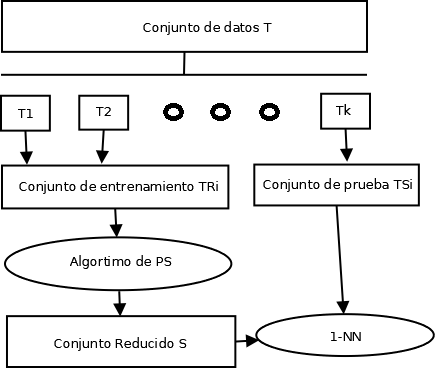
\includegraphics[scale=0.3]{classicCV.png}
\caption[Validación cruzada clásica]{Validación cruzada clásica}
\label{crossval}
\end{figure}

Por otra parte está la estratificación, la cual es una técnica propuesta por \emph{Cano, J. et al.} en \cite{cano2005stratification} para solventar el problema de aplicación de los algoritmos de PS frente a conjunto de datos muy grandes. Dicho problema viene dado porque la mayoría de los algoritmos de PS y metaheurísticas utilizadas son $O(n^2)$, siendo n la cantidad de instancias del conjunto a procesar, y por lo tanto, para grandes volúmenes de datos estos algoritmos empiezan a tardar mucho en computar una solución, lo cual los vuelve poco útiles al momento de hacer preprocesamiento de datos. Es así que la estratificación se adopta como una técnica que lleva a tiempos aceptables el cómputo con conjuntos de muchas instancias. 

Dado un conjunto de datos D, la estratificación empieza dividiendo D en k subconjuntos, llamados estratos, mutuamente exclusivos $D_1,D_2,\dots,D_k$ de aproximadamente el mismo tamaño y preservando la distribución de clases presente en D. Luego, a diferencia de la validación cruzada clásica que forma un conjunto TR a partir de k-1 subconjuntos $D_i$, para luego aplicar el algoritmo de PS, en la estratificación se aplica el algoritmo de PS directamente a cada uno de los $k-1$ subconjuntos seleccionados para el entrenamiento, formando entonces subconjuntos reducidos $DS_1,DS_2,\dots,DS_{t-1},DS_{t+1},\dots,DS_k$, donde $D_t$ es el conjunto seleccionado como conjunto de prueba; acto seguido, se juntan todos los $DS_i$ para formar el conjunto reducido S que va a ser usado por 1-NN para clasificar $D_t$. La estratificación prueba ser un método efectivo, como lo demuestran en \cite{cano2005stratification}, ya que reduce considerablemente la cantidad de instancias que debe tratar el algoritmo de PS a $\frac{N}{k}$, por lo que la elección del número de estratos k se vuelve de especial importancia. Para este trabajo se adopta k = 10 para los conjuntos medianos y k = 50 para los conjuntos grandes, tal y como se determinan en \cite{cano2005stratification}, cuya idea es hacer que cada algoritmo de PS no trabaje con más de 2000 instancias por estrato para reducir la cantidad a un conjunto de tamaño pequeño según la clasificación anteriormente expuesta. Además, al igual que en la validación cruzada clásica, las metaheurísticas utilizadas son estocásticas y por lo tanto, cada una de las k pruebas realizadas se repite 3 veces, regresando el promedio de todas las pruebas realizadas como resultado. En la figura \ref{strat} se muestra un esquema de cómo se aplica la estratificación, donde el estrato k es seleccionado como conjunto de prueba.

\begin{figure}[]
\centering
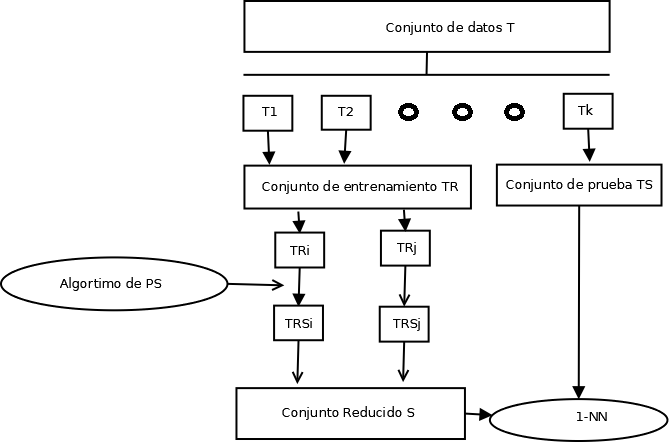
\includegraphics[scale=0.3]{stratCV.png}
\caption[Estratificación]{Estratificación}
\label{strat}
\end{figure}

\section{Entonación de las metaheurísticas}

Para la entonación de las metaheurísticas se uso \emph{irace} \cite{lopez2016irace}, el cual es un paquete de R que implementa el método de entonación automática conocido como \emph{iterated F-race}, el cual forma parte de los métodos de filtro según la taxonomía propuesta por \emph{Eiben, A. \& Smit, S.} en \cite{eiben2011parameter}. Como método de filtro, su principal objetivo es ir reduciendo los vectores de parámetros (configuraciones) a entonar paulatinamente, usando una competencia continua en la cual, cuando existen suficientes pruebas estadísticas de que una configuración genera una utilidad (evaluación de la función objetivo) con menos valor que el resto de las configuraciones, se elimina de las pruebas. Para mayor información respecto a la taxonomía de los métodos de entonación automática se recomienda leer \cite{eiben2011parameter}.


\emph{Iterated F-race} en específico trata de un método que consiste en tres pasos: (1) elegir varias configuraciones posibles de acuerdo a una distribución en particular y así formar una población, (2) elegir las mejores configuraciones de la población por medio de un proceso de carrera y (3) actualizar la distribución de la población de tal manera que se sesgue a favor de las mejores configuraciones. Estos tres pasos son repetidos hasta que un criterio de parada es cumplido. El algoritmo de \emph{iterated F-race} se presenta en \ref{irace}.

\begin{algorithm}
\caption{IRACE}
\label{irace}
\begin{algorithmic}[1]

\Require{\texttt{I} conjunto de instancias del problema a entonar, \texttt{X} espacio de configuraciones, U función de utilidad, \texttt{B} presupuesto con el que se cuenta}
\Ensure{$\theta^{elite}$ mejores configuraciones encontradas}

\State $\theta_1 \gets$ una muestra uniforme de X
\State $\theta^{elite} \gets$ resultado de una \textbf{carrera} usando $\theta_1$ como población y con presupuesto $B_1$
\State $j \gets 1$
\While{$B^{usado} \leq B$}
	\State $j \gets j + 1$
	\State $\theta^{nueva} \gets$ muestra sesgada hacia $\theta^{elite}$ de X 
	\State $\theta_j \gets \theta^{nueva} \cup \theta^{elite}$
	\State $\theta^{elite} \gets$ resultado de una \textbf{carrera} usando $\theta_j$ como población y con presupuesto $B_j$
\EndWhile
\State \Return $\theta^{elite}$

\end{algorithmic}
\end{algorithm}

\emph{Irace} empieza estimando cuántas iteraciones $N^{iter}$ va a ejecutar; este valor está en función al número de parámetros que se piensa entonar, por lo tanto $N^{iter} = \lfloor 2 + log_2 N^{parametros} \rfloor$, donde $N^{parametros}$ representa el número de parámetros, con la idea de que mientras más parámetros se necesite entonar, mayor será la cantidad de iteraciones que una carrera en específico necesita para conseguir las configuraciones élites. El cálculo de cuántas carreras se van a realizar en total, calculado $N^{iter}$, va en función de cuanto presupuesto B se le asigne a todo el proceso; se calcula la cantidad de carreras como $\lfloor B / N^{iter} \rfloor$. Si la cantidad de carreras es 0 entonces \emph{irace} pide que se introduzca un B mayor. Para este estudio, se asignó para los conjuntos pequeños y medianos $ B = 1000$ iteraciones y en cada carrera las metaheurísticas disponían de 1000 iteraciones para hallar el mejor valor posible; en cambio, para los conjuntos grandes se asignó $B = 400$ y cada metaherística en cada carrera disponía de 300 iteraciones.

Cabe acotar que \emph{irace} asume que el problema sobre el cual se va a entonar es un problema de minimización. Por lo tanto, siempre se busca menores valores de la función de utilidad U para cada configuración; además, luego de cada carrera asigna un rango $r_z$ dependiendo de cómo se compare la configuración z con respecto al resto, a menor rango, mejor es la configuración, por lo tanto, el conjunto de élites $\theta^{elite}$ está conformado por los k elementos con menor rango. El número k es calculado al principio de la corrida de \emph{irace} y en este trabajo se deja su cálculo automático por defecto.

Por otra parte,en la primera línea del algoritmo \ref{irace}, se hace un muestreo uniforme del espacio de configuraciones X con una distribución normal truncada. En las siguientes iteraciones se va sesgando el muestreo con las configuraciones élites encontradas en la línea 6, esto se logra usando una probabilidad $p_z$ con la cual se toma una configuración $ \theta^z$ que se calcula como en la ecuación (2.5), donde $N^{elite}_{j-1}$ es el número de élites de la iteración j-1:

\begin{equation}
p_z = \frac{N^{elite}_{j-1} - r_z + 1}{N^{elite}_{j-1}*\frac{N^{elite}_{j-1}+1}{2}}
\end{equation} 

Una vez obtenido un $\theta^z$ se genera una nueva configuración tomando una muestra del espacio de parámetros X, un parámetro d a la vez de entre un rango $[d_{inf},d^{sup}]$ definido por el usuario, usando una distribución normal truncada $\mathcal{N}(\mu^z_d,(\sigma^j_d)^2)$ donde $\mu^z_d$, que representa la media, es el valor $\theta^z_d$ y la variancia $\sigma^j_d$ está definida como $(d^{sup}-d_{inf}) / 2 $ en la iteración j, con una actualización progresiva  en cada iteración dada por la ecuación (2.6), donde $N^{nuevo}_j$ es el número de configuraciones en la población que se va a generar en la línea 6 del algoritmo \ref{irace} en la iteración j, con el fin de acercar cada vez más los nuevos elementos a la élite encontrada en las últimas iteraciones del experimento.

\begin{equation}
\sigma^j_d = \sigma^{j-1}_d *\left(\frac{1}{N^{nuevo}_j}\right)^{\frac{1}{N^{parametros}}}
\end{equation}

El proceso de carrera (\emph{racing} en inglés) para la entonación de metaheurísticas con el cual se realiza el paso (2) (líneas 2 y 8), fue propuesto por \emph{Birattari, M. et al.} en \cite{birattari2002racing}. La carrera empieza usando una población con configuraciones; luego, a cada iteración de la carrera, las configuraciones son evaluadas en una sola instancia $I_j$. Después de un número iteraciones dadas por un parámetro T, aquellas configuraciones que estadísticamente tienen un desempeño inferior al resto son descartadas. \emph{Irace} establece  $T = 1$; además, puede usar una prueba Friedman no paramétrica o una prueba t-test como prueba estadística para hacer las comparaciones entre las configuraciones. Por recomendación de los autores, se usa una prueba t-test con un valor de significancia de 0.05 ya que, según sus criterios, es la más adecuada para la entonación de parámetros de valores continuos.

\emph{Irace}, además, implementa un método de reinicialización cuando la población de configuraciones converge prematuramente. En este proceso se mantienen las configuraciones élites de la última carrera y empieza de nuevo segun ciertas consideraciones. Aunado a esto, \emph{irace} también implementa un sistema de carrera elitista, el cual evita que las mejores configuraciones encontradas hasta el momento se pierdan en una carrera producto de una serie desfavorable de evaluaciones en un momento dado. En este trabajo se usa ambas funciones como configuración por defecto que tiene \emph{irace}. Para más información de todas las funciones y utilidades que presenta esta herramemienta, se recomienda leer \cite{lopez2016irace}.

\chapter{Evaluación experimental}
\label{capitulo3}
\lhead{Capítulo 3. \emph{Evaluación experimental}}

\section{Diseño experimental}

En este capítulo se describen todas las decisiones tomadas con respecto a la experimentación; esto incluye los parámetros usados para la entonación, las particiones hechas en la validación cruzada y la estratificación, el diseño de los experimentos donde se combinan las heurísticas con las metaheurísticas y finalmente se presentan los resultados de cada prueba realizada. 

Lo primero que se hace es entonar los algoritmos evolutivos para que devuelvan el mejor valor posible al probarse con los conjuntos de datos presentados en la sección 2.4. Para lograr la entonación, se usa \emph{irace}, presentado en la sección 2.6, con los parámetros de la tabla \ref{irace-param}. Se consigue una configuración de parámetros para los problemas pequeños, medianos y grandes respectivamente.

\begin{table}[]
\centering
\begin{tabular}{l c}
\hline
Parámetros & irace \\
\hline
\hline
Iteraciones                                 &  1000, 400 y 100\\
Número decimales significativos             &    4            \\
Prueba estadística                          &  t-test         \\
Nivel de significancia para prueba estadística  &  0.05           \\
Frecuencia de la prueba estadística         &    1 iteración  \\
Número de configuraciones élites            &  automática     \\
Reinicialización por convergencia prematura &     Sí          \\
Modo elitista                               &     Sí          \\

\hline
\end{tabular}
\caption{Parámetros usados para \emph{irace}}
\label{irace-param}
\end{table}

Los parámetros a entonar son: número de iteraciones, cardinalidad de la población, probabilidad de cruce, probabilidad de mutación y tamaño del torneo. Los rangos válidos para cada parámetro se presentan en la tabla \ref{rangos}. La elección de los rangos se hace en base a los trabajos \cite{de2004reduccion,de2004reduccion,garcia2012prototype,garcia2008memetic,talbi2009metaheuristics}. Los resultados de la entonación se presentan en las tablas \ref{param-peq}, \ref{param-med} y \ref{param-grande}.

\begin{table}[]
\centering
\begin{tabular}{l c c}
\hline
Parámetros & Tipo de dato & Rangos \\
\hline
\hline

Población                & entero           &  [10,150]       \\
Probabilidad de cruce    & real             &  [0,1]          \\
Probabilidad de mutación & real             &  [0,0.01]      \\
Número del torneo        & entero           &  [1,10]         \\  

\hline
\end{tabular}
\caption{Rangos usados para los parámetros en la entonación}
\label{rangos}
\end{table}

\begin{table}[]
\centering
\begin{tabular}{l c c c c}
\hline
\multirow{2}{*}{\textsc{Parámetros}}
	& \multicolumn{4}{c}{\textsc{Algoritmos}} \\
	& GGA & SGA & MA & CHC \\
\hline
\hline
Iteraciones             &  1000    &  1000    &  1000      &  1000 \\
Población               &    70    &    90    &    21      &    33 \\
Prob. de Cruce          &   0.4837 &   0.9848 &     0.9496 &     - \\
Prob. de Mutación       &   0.0001 &  0.0057  &     0.0071 &     - \\
Número del torneo       &   -      &    3     &     1      &     - \\
\hline
\end{tabular}
\caption{Parámetros usados para los conjuntos pequeños}
\label{param-peq}
\end{table}


\begin{table}[]
\centering
\begin{tabular}{l c c c c}
\hline
\multirow{2}{*}{\textsc{Parámetros}}
	& \multicolumn{4}{c}{\textsc{Algoritmos}} \\
	& GGA & SGA & MA & CHC \\
\hline
\hline
Iteraciones             &  1000    &  1000    &  1000      &  1000 \\
Población               &    88    &    132   &    32      &    27 \\
Prob. de Cruce          &   0.5779 &   0.9859 &     0.9549 &     - \\
Prob. de Mutación       &   0.0001 &  0.0001  &     0.0004 &     - \\
Número del torneo       &   -      &    1     &     3      &     - \\
\hline
\end{tabular}
\caption{Parámetros usados para los conjuntos medianos}
\label{param-med}
\end{table}

\begin{table}[]
\centering
\begin{tabular}{l c c c c}
\hline
\multirow{2}{*}{\textsc{Parámetros}}
	& \multicolumn{4}{c}{\textsc{Algoritmos}} \\
	& GGA & SGA & MA & CHC \\
\hline
\hline
Iteraciones             &  1000    &  1000    &  1000      &  1000 \\
Población               &    102   &    122   &    35      &    37 \\
Prob. de Cruce          &   0.5158 &   0.9554 &     0.9698 &     - \\
Prob. de Mutación       &   0.0001 &  0.0078  &     0.0049 &     - \\
Número del torneo       &   -      &    7     &     3      &     - \\
\hline
\end{tabular}
\caption{Parámetros usados para los conjuntos grandes}
\label{param-grande}
\end{table}

Para la validación cruzada se usa k = 10 y se repite cada prueba 3 veces basándose en el trabajo de \emph{Cano, J.} en \cite{de2004reduccion}. Este esquema de validación cruzada se aplica a los conjuntos de tamaño pequeño como lo hacen en \cite{de2004reduccion}. Para la estratificación se adopta k = 10 para los conjuntos medianos y k = 50 para los conjuntos grandes, tal y como se determinan en \cite{cano2005stratification}, cuya idea es hacer que el algoritmo de PS no trabaje con más de 2000 instancias por estrato para reducir la cantidad a un conjunto de tamaño pequeño según la clasificación anteriormente expuesta. Además, al igual que en la validación cruzada, las metaheurísticas utilizadas son estocásticas y por lo tanto, cada una de las k pruebas realizadas se repite 3 veces, con lo que se regresa el promedio de todas las pruebas realizadas como resultado.

Una vez obtenido los distintos parámetros para cada metaheurística, se procede con el experimento principal, el cual consiste en mejorar la población inicial de las metaheurísticas GGA, SSGA, MA y CHC por medio de las heurísticas CNN, ENN y RSS quienes seleccionan soluciones prometedoras del espacio de soluciones factibles.

La selección de CNN, ENN, y RSS se debe a que son de las heurísticas que emplean menores tiempos en su selección según el trabajo de \emph{Salvador, G. et al.} en \cite{garcia2012prototype} y por el tipo de instancias que eligen: la primera heurística elige las instancias bordes mientras que descarta las instancias internas bajo la idea de que las instancias bordes son las que realmente establecen los límites de decisión entre clases; ENN por su parte, elige las instancias internas y se deshace de las instancias bordes con la premisa de que las instancias bordes sólo agregan ruido al conjunto y por lo tanto hay que eliminarlas; por último RSS es un híbrido que preserva algunas instancias bordes y algunas instancias internas, con lo que mantiene una distancia uniforme entre las mismas. En la figura \ref{heu} se puede apreciar la selección de instancias realizadas por cada heurística sobre el conjunto banana, la cual refleja lo explicado anteriormente.

\begin{figure}[]

	\centering
	\subfigure[Banana]{\label{fig:a}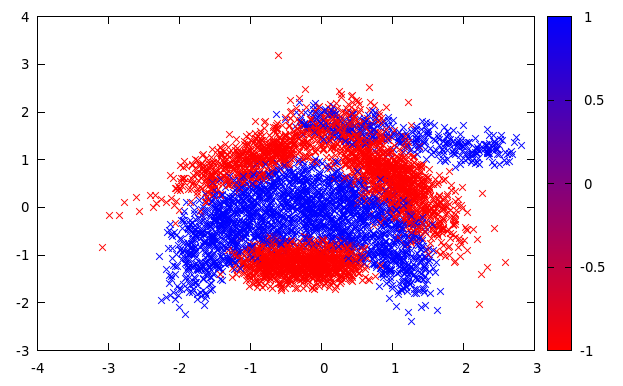
\includegraphics[scale=0.3]{banana.png}}
	\subfigure[CNN]{\label{fig:b}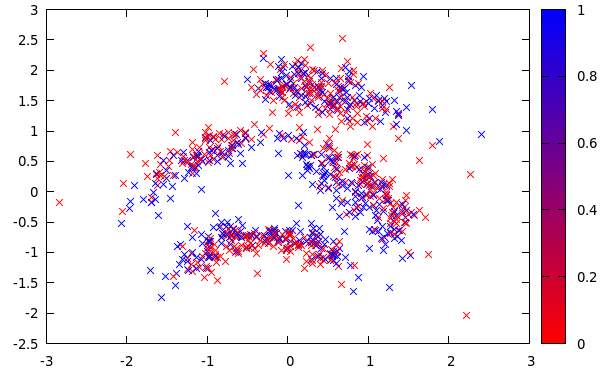
\includegraphics[scale=0.3]{CNN.png}}
	\subfigure[ENN]{\label{fig:c}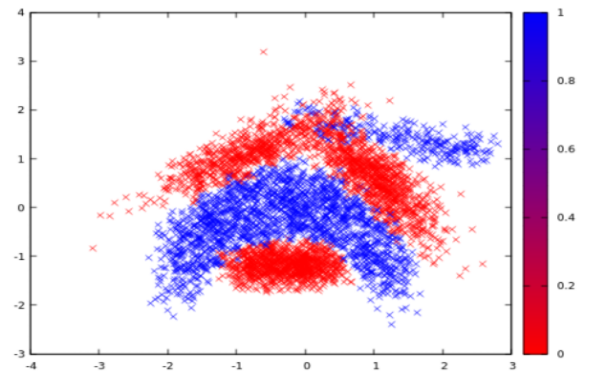
\includegraphics[scale=0.3]{ENN.png}}
	\subfigure[RSS]{\label{fig:d}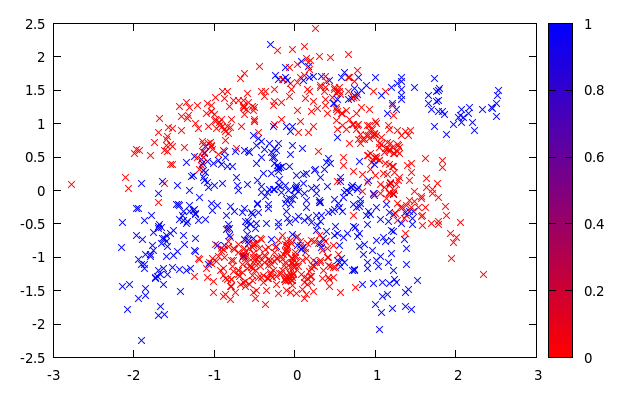
\includegraphics[scale=0.3]{RSS.png}}

\caption{Selección de instancias de las heurísticas}
\label{heu}
\end{figure}


Para presentar los resultados, se usan tablas que contienen los promedios en \emph{accuracy}, \emph{kappa}, reducción y tiempo de cómputo medido en segundos para cada heurística. \emph{Accuracy y kappa} se miden sobre los conjuntos de entrenamiento y prueba, la reducción mide el porcentaje de instancias eliminadas del conjunto original; a mayor \emph{accuracy, kappa} y reducción mejor es la heurística. Las pruebas fueron realizadas para los conjuntos pequeños, medianos y grandes por separado. Además, para determinar cuál si una metaheurística es mejor que otra se utiliza una prueba de \emph{Wilcoxon} de rango con signo con un nivel de significacia de 1\%, donde la hipótesis nula implica que las medidas son estadísticamente iguales y la hipótesis alternativa indica que existe una diferencia real entre las medidas.

Los experimentos fueron hechos con un procesador Intel(R) Core(TM) i5-3470 CPU @ 3.20GHz, 4 procesadores y 4GB de memoria RAM. Se utilizó C++ como lenguaje de programación y se compiló con GCC v.7.3.0.

\section{Resultados}

\subsection{Heurísticas}

En esta sección se busca estudiar el comportamiento de CNN, ENN y RSS al ser usados para resolver el problema de selección de prototipos sobre conjuntos de datos de tamaño pequeño, mediano y grande. De los resultados obtenidos, se espera determinar cuál heurística presenta los mejores niveles de \emph{accuracy, kappa} y reducción; además se busca evaluar el tiempo de cómputo de cada heurística.


\begin{table}[h!]
\centering
\begin{tabular}{l c c c c c c}
\hline
\multirow{2}{*}{\textsc{Algoritmo}}
	& \multicolumn{2}{c}{\textsc{Accuracy}}
	& \multicolumn{2}{c}{\textsc{Kappa}}
	& \textsc{Reducción}
	& \textsc{Tiempo (seg)} \\
	& Training & Test
	& Training & Test \\ 
\hline
\hline

Pequeños\\
CNN & 0.9093 & 0.7447 & 0.8396 & 0.5404 & 0.7380 & 0.1351 \\
ENN & 0.8563 & 0.7924 & 0.7319 & 0.6120 & 0.2591 & 0.1815 \\
RSS & 0.8363 & 0.7499 & 0.6997 & 0.5426 & 0.7308 & 0.1231 \\

\hline

Medianos\\
CNN & 0.8944 & 0.7823 & 0.7611 & 0.5613 & 0.7437 & 0.7108 \\
ENN & 0.8402 & 0.7999 & 0.6842 & 0.5863 & 0.2861 & 1.2668 \\
RSS & 0.8619 & 0.7922 & 0.6822 & 0.5524 & 0.6477 & 0.9201 \\

\hline

Grandes\\
CNN & 0.8818 & 0.8158 & 0.7396 & 0.5587 & 0.8183 & 3.2853 \\
ENN & 0.9355 & 0.8895 & 0.7938 & 0.6463 & 0.1495 & 6.1658 \\
RSS & 0.9176 & 0.8731 & 0.7411 & 0.6007 & 0.7236 & 10.7264 \\


\hline
\end{tabular}
\caption{Promedios de heurísticas}
\label{heu}
\end{table}

Al estudiar los resultados presentes en la tabla \ref{heu}, se puede destacar:

\begin{itemize}

\item ENN es la heurística que presenta los mejores niveles de \emph{accuracy y kappa} en la validación (\emph{test}) para los conjuntos de los tres tamaños. Esto se debe a que ENN es la heurística que menos instancias elimina y por lo tanto el conjunto $S$ resultante se asemeja bastante al conjunto original, lo cual le permite mantener buenos niveles de representación.

\item CNN es la heurística que tiene los mayores niveles de reducción. Además, se puede observar que CNN presenta sobre-entrenamiento (\emph{overfitting}) tanto en \emph{accuracy} como en \emph{kappa}; lo cual se hace evidente por la marcada diferencia entre los valores obtenidos en los conjuntos de entrenamiento (\emph{training}) y los valores obtenidos en los conjuntos de validación (\emph{test}), donde 29.92\% es la diferencia más grande presente en el \emph{kappa} para los conjuntos pequeños. Tanto los buenos niveles de reducción como el sobre-entrenamiento suceden porque CNN elige sólo las instancias limítrofes entre clases para construir el conjunto $S$, donde elimina la mayoría de las instancias, que se concentran en la parte interna del espacio y por lo tanto, pierde parte del nivel de representación del conjunto original.

\item RSS presenta niveles similares de \emph{accuracy y kappa} a los vistos para CNN en los conjuntos pequeños y medianos, y niveles superiores en los conjuntos grandes. Por otra parte, presenta niveles superiores de reducción a los vistos para ENN. RSS representa un balance entre \emph{accuracy, kappa} y reducción producto de una selección mixta de instancias internas y limítrofes.


\end{itemize}

En conclusión, si se busca mantener los mejores niveles de \emph{accuracy y kappa} sin importar los niveles de reducción, ENN es la opción indicada porque mantiene casi todo el conjunto original intacto. En cambio, si se busca la máxima reducción posible, al dejar en segundo plano el \emph{accuracy y kappa}, CNN es la opción sugerida. Sin embargo, para mantener un equilibrio entre las tres mediciones, RSS es la mejor opción.

Al evaluar los tiempos de cómputo presentes en la tabla \ref{heu} se pueden observar los siguientes detalles:

\begin{itemize}

\item CNN es la heurística más rápida y es la que mejor escala a conjuntos de tamaño grande. Su rapidez sucede porque el algoritmo empieza con un conjunto vacío y agrega instancias conforme a los errores de clasificación que encuentra en cada iteración, deteniéndose cuando logra pasar una iteración sin errores. Este esquema le permite a CNN terminar rápidamente en la mayoría de los casos, independientemente del tamaño del conjunto a reducir, porque el conjunto de referencia con el que se hacen las clasificaciones siempre se mantiene pequeño. Se debe acotar que CNN, siendo un algoritmo con componentes estocásticos, puede tardar más del tiempo esperado en dar una solución porque, dependiendo del orden de presentación de las instancias, CNN puede llegar a necesitar varios iteraciones sobre el conjunto original para terminar; para casos patológicos, CNN puede llegar a tener una complejidad de $O(n^2*log(n))$, cuando el tiempo esperado normalmente es de $O(n*log(n))$.

\item ENN presenta los segundos mejores tiempos entre las tres heurísticas. EL tiempo adicional que le toma a ENN devolver una solución en comparación a CNN se debe a que ENN empieza con el conjunto original en su totalidad y en cada iteración elimina una instancia que no concuerda con la clase de su vecino más cercano. Sin embargo, como ENN sólo tiene que revisar cada instancia una sola vez, puede terminar en un buen tiempo inclusive con los conjuntos grandes. ENN tiene una complejidad de $O(n*log(n))$  

\item RSS es la heurística que peor escala entre las tres, ya que el tiempo que se requiere para terminar con un conjunto grande 10 veces más el tiempo requerido por un conjunto mediano. Este detalle de escalabilidad se debe a que RSS primero debe ordenar todas las instancias según la distancia a sus enemigos más cercanos, lo cual domina el tiempo del algoritmo y asintóticamente lo vuelve $O(n*log(n))$. Sin embargo, hay que tomar en cuenta que los tiempos son buenos para los conjuntos grandes, ya que regresa un resultado en aproximadamente 10 segundos; tiempo que es significativamente menor a lo requerido por los algoritmos evolutivos, como se verá en las secciones siguientes.

\end{itemize}

Una vez considerado los tiempos, se concluye que las tres heurísticas son una opción viable para reducir los datos dependiendo de las prioridades del usuario como se explicó anteriormente. Inclusive, los problemas de escalamiento presentes en RSS son mitigados con el uso de la estratificación, por lo que es la mejor opción si el usuario busca un balance entre \emph{accuracy, kappa} y reducción.



\subsection{Metaheurísticas}

En esta sección se estudia el comportamiento de GGA, SSGA, MA y CHC, con población inicial aleatoria, al resolver el problema de selección de instancias sobre conjuntos pequeños, medianos y grandes. El objetivo es determinar cuál algoritmo presenta los mejores niveles de \emph{accuracy, kappa} y reducción para los conjuntos de los distintos tamaños. Además, se estudia el tiempo que requiere cada algoritmo en dar una solución, con lo que se busca evaluar si hay una buena relación entre tiempo y calidad de los resultados.


\begin{table}[h!]
\centering
\begin{tabular}{l c c c c c c}
\hline
\multirow{2}{*}{\textsc{Algoritmo}}
	& \multicolumn{2}{c}{\textsc{Accuracy}}
	& \multicolumn{2}{c}{\textsc{Kappa}}
	& \textsc{Reducción}
	& \textsc{Tiempo (seg)} \\
	& Training & Test
	& Training & Test \\ 
\hline
\hline

Pequeños\\
GGA  & 0.8312 & 0.7525 & 0.7017 & 0.5557 & 0.5532 & 12.8250 \\
SSGA & 0.8654 & 0.7716 & 0.7635 & 0.5917 & 0.8432 & 0.6655 \\
MA   & 0.8570 & 0.7918 & 0.7440 & 0.6216 & 0.9561 & 4.1047 \\
CHC & 0.8446 & 0.7843 & 0.7172 & 0.6084 & 0.9466 & 0.5266 \\

\hline

Medianos\\
GGA  & 0.8702 & 0.7982 & 0.7375 & 0.5812 & 0.5641 & 110.0812 \\
SSGA & 0.8431 & 0.8029 & 0.6676 & 0.5871 & 0.8392 & 3.5589 \\
MA   & 0.8057 & 0.7908 & 0.5825 & 0.5564 & 0.9624 & 73.3461 \\
CHC  & 0.8313 & 0.8115 & 0.6347 & 0.5986 & 0.9455 & 2.8843 \\

\hline
Grandes\\
GGA  & 0.9316 & 0.8644 & 0.7994 & 0.6014 & 0.5050 & 672.0273 \\
SSGA & 0.8911 & 0.8743 & 0.6953 & 0.6201 & 0.8056 & 27.6637 \\
MA   & 0.8904 & 0.8999 & 0.6499 & 0.6510 & 0.9973 & 256.1432 \\
CHC  & 0.8961 & 0.8934 & 0.6614 & 0.6506 & 0.9615 & 16.8665 \\

\hline
\end{tabular}
\caption{Promedios de las metaheurísticas}
\label{meta}
\end{table}

Al estudiar los resultados obtenidos en la tabla \ref{meta}, se puede destacar:

\begin{itemize}

\item CHC y MA presentan los mejores niveles de \emph{accuracy y kappa} para los conjuntos de validación pequeños y grandes. Esto se atribuye a los mecanismos internos que tiene cada algoritmo para hacer la mejor selección de instancias posible. MA tiene su función de optimización que elimina todas las instancias posibles sin perjudicar el \emph{accuracy}, lo que permite mejorar al máximo cada cromosoma de la población; mientras que CHC tiene su mecanismo de prevención de incesto para crear cromosomas lo más distinto posible de los padres, además de tener la capacidad de reiniciar su población, tomando como base el mejor cromosoma encontrado, para evitar la convergencia prematura de la misma.

\item SSGA presenta niveles similares de \emph{accuracy y kappa} que GGA para los conjuntos de validación de pequeños y grandes. Ambos algotirmos presentan niveles inferiores que CHC y MA producto de una selección de instancias menos informada que estos últimos. La única manera estable que tienen GGA y SSGA para obtener mejores resultados es a través de la operación de cruce, mientras que MA y CHC cuentan con las herramientas antes mencionadas.

\item Para los conjuntos medianos, las cuatro metaheurísticas obtuvieron un nivel de \emph{accuracy} similar. Mientras que MA obtuvo un nivel de \emph{kappa} inferior a los otros tres métodos. Este comportamiento de las metaheurísticas frente a los conjuntos medianos se atribuye directamente a la topología (cómo se encuentran organizadas las soluciones en el espacio) de los conjuntos de datos utilizados para realizar las pruebas; lo que deja en evidencia la influencia que tiene el conjunto de datos sobre el comportamiento de los algoritmos.

\item MA es la metaheurística que presenta los mayores niveles de reducción. Este hecho se vuelve a atribuir a el proceso de optimización interna, ya que es un proceso de intensificación en el cual se refina un cromosoma a uno con la mínima cardinalidad posible sin perder \emph{accuracy}.

\item CHC alcanza buenos niveles de reducción, gracias a la selección totalmente elitista de los cromosomas que siempre realiza en cada iteración (sólo se preservan los mejores cromosomas y es a partir del mejor que se reinicia la población). Como uno de los componentes que comforma la función objetivo es la tasa de reducción, CHC naturalmente favorece aquellas soluciones con pocas instancias que puedan mantener buenos valores de \emph{accuracy y kappa}.

\item GGA presenta los niveles más bajos de reducción, esto ocurre porque no posee mecanismos de preservación elitistas como en el caso de CHC. GGA se caracteriza por perder toda la información acumulada en una generación de cromosomas (excepto el mejor), eliminando cromosomas que podrían generar mejores soluciones si se les diera más oportunidades de ser cruzados. Además, GGA carece de procesos de intensificación como los tiene MA, lo cual vuelve más difícil la eliminación de instancias.

\item SSGA presenta mejores niveles de reducción a los obtenidos por GGA porque usa un método simple de elitismo, en el cual en cada iteración sólo se generan dos cromosomas nuevos (a diferencia de una población entera) y éstos sólo suplantan a sus padres si son mejores. Este mecanismo permite que la cantidad de instancias disminuya paulatinamente hasta llegar a la convergencia de la población.

\item CHC es la metaheurística que necesita menos tiempo en dar una solución. Esto se debe a su operador de cruce, el cual tarda tiempo lineal ($O(n)$) y permite hacer una búsqueda diversificada del espacio de soluciones de manera inteligente, ya que, a partir de unos cromosomas seleccionados de manera elitista, genera nuevos cromosomas que son lo más distinto posible, mientras mantiene cualidades (las cuales se esperan que sean buenas) de sus padres. Estos detalles hacen posible la obtención de buenos resultados rápidamente.

\item SSGA es otra metaheurística que no necesita mucho tiempo en dar una solución. La razón de esto es parecida a la de CHC, ya que el operador de cruce toma tiempo lineal y en cada iteración sólo se generan 2 cromosomas, lo cual lleva al algoritmo a terminar rápidamente.

\item MA tarda significativamente más en regresar una solución en comparación a CHC y SSGA. Para los conjuntos pequeños, MA tarda 7 veces más que CHC; para los conjuntos medianos, MA tarda 25 veces más que CHC y para los conjuntos grandes, MA tarda 15 veces más. Esta diferencia en tiempo se debe al proceso de optimización interna que usa MA en cada iteración, el cual es $O(n^2)$.

\item GGA es la metaheurística que más tarda en dar una solución. Esto se debe a que en cada iteración, GGA debe generar una población de cromosomas nuevo, a diferencia de SSGA que sólo genera dos cromosomas.

\item CHC y SSGA son las metaheurísticas que mejor escalan a los conjuntos grandes, ya que mantienen los tiempos de ejecución por debajo de 30 segundos, teniendo valores no muy alejados de los tiempos obtenidos por las heurísticas. Por otra parte, GGA y MA sobrepasan los 200 segundos en tiempo de cómputo, lo cual es 20 veces más lo que tardan CNN, ENN y RSS. Sin embargo, hay que tomar en cuenta que la estratificación ayuda a reducir significativamente los tiempos de cómputo de las cuatro metaheurísticas, al punto de que es factible aplicar los cuatro algoritmos a los conjuntos grandes; ya que en trabajos como los realizados por \emph{Cano, J. et al.} en \cite{garcia2008memetic} y \cite{garcia2012prototype} no se pudo probar estos algoritmos sin el uso de estratificación por la gran cantidad de tiempo que tomarían en devolver una respuesta.

\end{itemize}


\begin{figure}[h!]

	\centering
	\subfigure[\emph{Accuracy} + reducción]{\label{fig:a}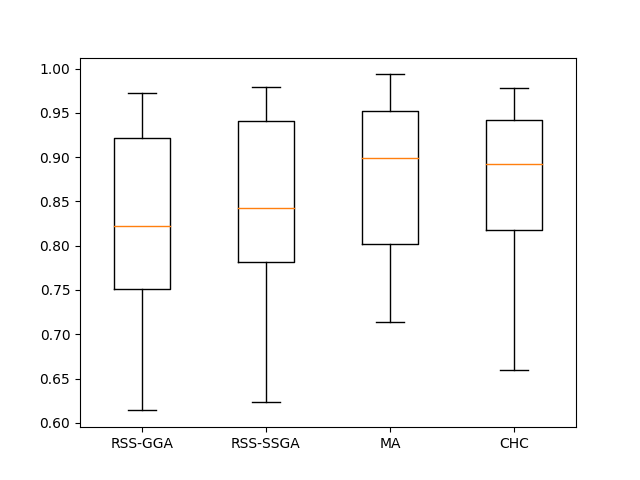
\includegraphics[scale=0.4]{acc_small.png}}
	\subfigure[\emph{kappa} + reducción]{\label{fig:b}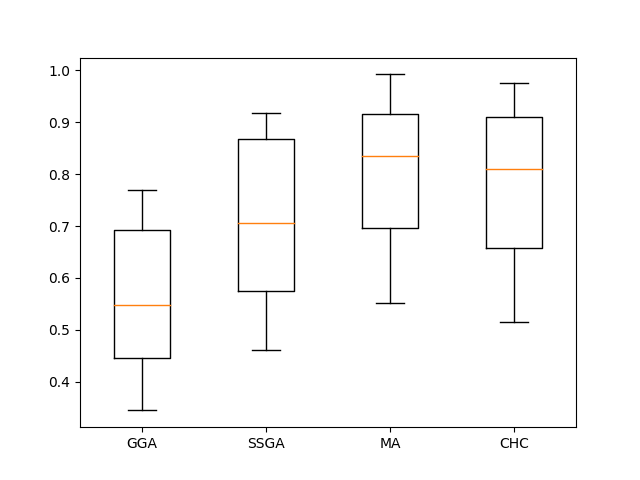
\includegraphics[scale=0.4]{kappa_small.png}}

\caption{Boxplots de las metaheurísticas para los conjuntos pequeños}
\label{small-heuristics}
\end{figure}

\begin{figure}[h!]

	\centering
	\subfigure[\emph{Accuracy} + reducción]{\label{fig:a}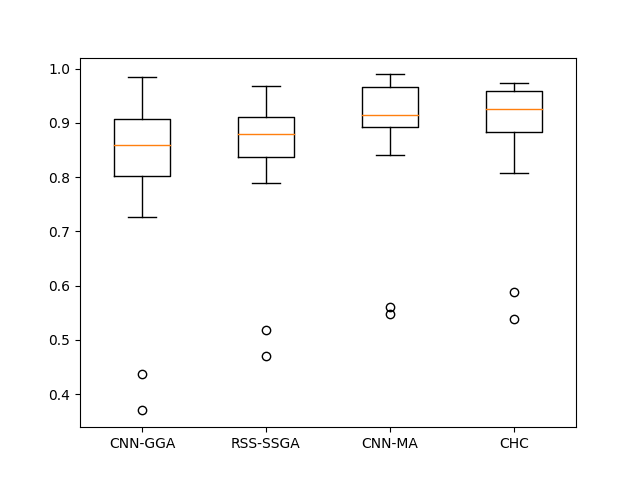
\includegraphics[scale=0.4]{acc_medium.png}}
	\subfigure[\emph{kappa} + reducción]{\label{fig:b}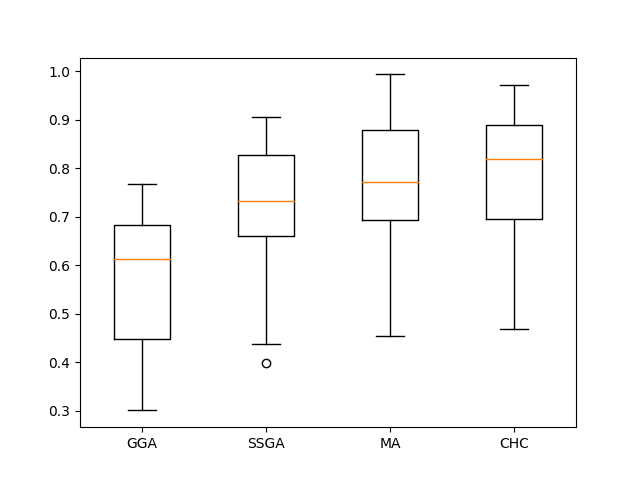
\includegraphics[scale=0.4]{kappa_medium.png}}

\caption{Boxplots de las metaheurísticas para los conjuntos medianos}
\label{medium-heuristics}
\end{figure}

Las figuras \ref{small-heuristics} y \ref{medium-heuristics} muestran que cuando se toma en cuenta la combinación lineal de \emph{accuracy} + reducción y \emph{kappa} + reducción, MA y CHC presentan los niveles más elevados. Cabe destacar que las tablas \ref{wilcox-meta-peq} y \ref{wilcox-meta-med} del Apéndice A muestran que los p-valores de la comparación entre MA y CHC para los conjuntos pequeños son 6.934e-02 para \emph{accuracy} + reducción y  7.80e-02 para \emph{kappa} + reducción. Por su parte, para los conjuntos medianos se tiene 6.009e-01 y 7.172e-01 respectivamente; lo cual implica que MA y CHC son estadísticamente similares. 

De acuerdo a la información presentada anteriormente, se puede concluir que CHC es la mejor metaheurística para resolver el problema de selección de prototipos para los conjuntos pequeños, medianos y grandes. Ya que, junto a MA presenta los valores más elevados de \emph{accuracy, kappa} y reducción, con la peculiaridad de que es la metaheurística que menos tiempo tarda en regresar un resultado. Lo cual lo hace el candidato ideal al momento de aumentar el tamaño de los conjuntos de datos.  



\subsection{Variaciones de las metaheurísticas}

Después del proceso anterior, el paso inmediato a seguir es la combinación de las heurísticas con las metaheurísticas. La idea es evaluar las variaciones de cada metaheurística por separado, de tal manera de que se se identifique cuál heurística beneficia más a la metaheurística. La notación en la columna de ``\textsc{Algoritmo}'' indica primero qué heurística se usó para inicializar la población y le sigue la metaheurística usada; un ejemplo es CNN-GGA, que indica que CNN es la heurística usada para inicializar la población de la metaheurística GGA. Para el caso de usar una población incial aleatoria, se coloca simplemente el nombre de la metaheurística. La mejor variación de cada metaheurística se encuentra sombreada.


\subsubsection{Conjuntos pequeños}

En esta sección se estudia el comportamiento de las variaciones de GGA, SSGA, MA y CHC al resolver el problema de selección de instancias sobre conjuntos pequeños. El objetivo es determinar cuál algoritmo presenta los mejores niveles de \emph{accuracy, kappa} y reducción. Además, se estudia el tiempo que requiere cada algoritmo en dar una solución, con lo que se busca evaluar si hay una buena relación entre tiempo y calidad de los resultados.


\begin{table}[h!]
\centering
\begin{tabular}{l c c c c c c}
\hline
\multirow{2}{*}{\textsc{Algoritmo}}
	& \multicolumn{2}{c}{\textsc{Accuracy}}
	& \multicolumn{2}{c}{\textsc{Kappa}}
	& \textsc{Reducción}
	& \textsc{Tiempo (seg)} \\
	& Training & Test
	& Training & Test \\ 
\hline
\hline

\textbf{GGA}         & \textbf{0.8312} & \textbf{0.7525} & \textbf{0.7017} & \textbf{0.5557} & \textbf{0.5532} & \textbf{12.8250} \\
CNN-GGA     & 0.5736 & 0.4911 & 0.3525 & 0.2151 & 0.7491 & 33.4671 \\
ENN-GGA     & 0.8533 & 0.7891 & 0.7327 & 0.6093 & 0.2611 & 14.6024 \\
RSS-GGA     & 0.6626 & 0.6177 & 0.4044 & 0.3263 & 0.7717 & 21.5376 \\
CNN-RSS-GGA & 0.7883 & 0.6809 & 0.6353 & 0.4472 & 0.6221 & 43.1002 \\
ENN-RSS-GGA & 0.8973 & 0.7872 & 0.8182 & 0.6063 & 0.1994 & 36.5439 \\

\hline

SSGA & 0.8654 & 0.7716 & 0.7635 & 0.5917 & 0.8432 & 0.6655 \\
CNN-SSGA & 0.8791 & 0.7695 & 0.7840 & 0.5815 & 0.8425 & 1.2187 \\
ENN-SSGA & 0.8733 & 0.7919 & 0.7683 & 0.6112 & 0.7823 & 0.8601 \\
\textbf{RSS-SSGA} & \textbf{0.8581} & \textbf{0.7726} & \textbf{0.7460} & \textbf{0.5905} & \textbf{0.8958} &\textbf{1.0116} \\
CNN-RSS-SSGA & 0.8808 & 0.7742 & 0.7884 & 0.5974 & 0.8373 & 1.9109 \\
EEN-RSS-SSGA & 0.8843 & 0.7890 & 0.7904 & 0.6134 & 0.7586 & 1.6563 \\

\hline

\textbf{MA}   & \textbf{0.8570} & \textbf{0.7918} & \textbf{0.7440} & \textbf{0.6216} & \textbf{0.9561} & \textbf{4.1047} \\
CNN-MA & 0.8653 & 0.7987 & 0.7519 & 0.6307 & 0.9486 & 5.9638 \\
ENN-MA & 0.8666 & 0.7930 & 0.7576 & 0.6215 & 0.9534 & 4.2491 \\
RSS-MA & 0.8446 & 0.7795 & 0.7137 & 0.5903 & 0.9630 & 4.6391 \\
CNN-RSS-MA  & 0.8639 & 0.7848 & 0.7538 & 0.6090 & 0.9507 & 8.9884 \\
ENN-RSS-MA & 0.8736 & 0.7942 & 0.7716 & 0.6268 & 0.9474 & 8.3942 \\

\hline

\textbf{CHC} & \textbf{0.8446} & \textbf{0.7843} & \textbf{0.7172} & \textbf{0.6084} & \textbf{0.9466} & \textbf{0.5266} \\
CNN-CHC & 0.8495 & 0.7812 & 0.7269 & 0.6027 & 0.9385 & 0.7891 \\
ENN-CHC & 0.8429 & 0.7863 & 0.7179 & 0.6132 & 0.9424 & 0.7445 \\
RSS-CHC & 0.8383 & 0.7779 & 0.6963 & 0.5836 & 0.9546 & 0.7137 \\
CNN-RSS-CHC  & 0.8442 & 0.7794 & 0.7099 & 0.5864 & 0.9437 & 1.1144 \\
ENN-RSS-CHC & 0.8484 & 0.7846 & 0.7224 & 0.6030 & 0.9333 & 1.0723 \\

\hline
\end{tabular}
\caption{Promedios de las distintas variaciones de cada metaheurística para los conjuntos pequeños}
\label{peq-all}
\end{table}

Al estudiar los resultados obtenidos en la tabla \ref{peq-all}, se pueden destacar los siguientes aspectos observados de las variaciones de GGA:

\begin{itemize}

\item GGA, ENN-GGA y ENN-RSS-GGA presentan los mejores niveles de \emph{accuracy y kappa}. Esto se debe a que son las variantes que preservan la mayor cantidad de instancias y por lo tanto el resultado mantiene un buen nivel de representación del conjunto original.

\item CNN-GGA presenta los niveles más bajos de \emph{accuracy}. Esto sucede porque la población inicial es bastante reducida y concentrada en las fronteras, debido a CNN, y GGA no posee los mecanismos para diversificar la población en búsqueda de mejores soluciones.

\item CNN-GGA y RSS-GGA presentan los niveles más bajos de \emph{kappa}, lo cual significa que los dos algoritmos generan conjuntos que incluyen principalmente elementos de la clase mayoritaria, dejando pocos representantes de las clases minoritarias que no ayudan a la correcta clasificación de las mismas. Estos valores por debajo del 35\% implican que entre los conjuntos pequeños hay conjuntos que están sesgados hacia una o más clases y los conjuntos construidos por CNN-GGA y RSS-GGA no logran representar correctamente las clases minoritarias.

\item RSS-GGA presenta los mejores niveles de reducción. Esto ocurre porque la selección mixta de instancias que hace RSS le permite a GGA tener una búsqueda diversificada por el espacio de soluciones, lo que facilita la obtención de resultados con menos instancias.

\item CNN-GGA también presenta buenos niveles de reducción porque CNN realiza casi toda la selección de instancias desde el principio.

\item ENN-GGA y ENN-RSS-GGA presentan las tasas más bajas de reducción. Esto ocurre porque ENN naturalmente deja la mayor cantidad de instancias y GGA carece de los medios para realizar una reducción significativa de un conjunto densamente poblado.

\item ENN-GGA y RSS-GGA son las variaciones, excluyendo a GGA, que menos tiempo toman en dar un resultado porque tanto ENN como RSS tienen una complejidad de $O(n*log(n))$ los cuales les permite devolver una respuesta rápidamente.

\item CNN-GGA tarda más que ENN-GGA y que RSS-GGA por una combinación de factores que incluyen: los componentes estocásticos de CNN, que pueden ocasionar una elevada cantidad de iteraciones hasta converger a un conjunto; y la probabilidad de cruce elegida para GGA, la cual es de 48.37\%, lo trae como consecuencia que pasen muchas iteraciones intentando cruzar cromosomas para formar todos los elementos de cada generación. Cabe destacar que el promedio de tiempo de cómputo de CNN-GGA se ve afectado por dos casos atípicos: \emph{Banknote} y \emph{Winsconsin} para los cuales se reportan 280.39 segundos y 272.64 segundos (véase tabla \ref{res-peq-cnn-gga} en el apéndice B) para que el algoritmo culmine.

\end{itemize}

De las observaciones anteriores se puede concluir que GGA con población inicial aleatoria es la mejor variación de GGA; esto se debe a que presenta el mejor balance entre \emph{accuracy, kappa} y reducción, además de que es la variente más rápida. El uso de heurísticas en este caso, no representa una mejoría significativa por el cual se justifique el costo adicional en tiempo que conlleva el uso de las heurísticas; las mismas introducen desequilibrios al enofarse únicamente en \emph{accuracy y kappa} (como el caso de ENN-GGA) o en reducción (como el caso de CNN).

Al pasar a los resultados obtenidos para las variaciones de SSGA, se puede observar:

\begin{itemize}

\item ENN-SSGA y ENN-RSS-SSGA presentan los mejores valores para \emph{accuracy y kappa} producto de usar un conjunto inicial con la mayoría de las instancias del conjunto original.

\item RSS-SSGA presenta la tasa de reducción más alta, gracias a la selección de instancias realizada por RSS, la cual introduce variedad en la búsqueda de SSGA.

\item La diferencia entre la tasa más alta y la más baja de reducción es de 13.72\%, siendo la tasa más baja la de ENN-RSS-SSGA con 75.86\%. Este resultado muestra que SSGA puede conseguir buenas tasas de reducción inclusive con un conjunto inicial muy parecido al conjunto original en cardinalidad.

\item Los mejores tiempos entre las variantes que usan heurísticas son los obtenidos por ENN-SSGA y RSS-SSGA, las razones son las mismas que las dadas para las variaciones de GGA. 

\end{itemize}

De las consideraciones anteriores, se puede concluir que RSS-SSGA es la mejor variación de SSGA, ya que presenta la mayor tasa de reducción, estando 5.26\% por encima de SSGA con población inicial aleatoria, y mantiene buenos niveles de \emph{accuracy y kappa}, razones que justifican el tiempo adicional de cómputo, que cabe destacar está por debajo de los dos segundos, lo que lo posiciona entre las metaheurísticas más rápidas.

Al evaluar los resultados obtenidos por las variaciones de MA, se observa:

\begin{itemize}

\item Todas las variaciones presentan valores similares de \emph{accuracy y kappa}. El mayor \emph{accuracy}, obtenido por ENN-RSS-MA, sólo está 0.24\% por encima del \emph{accuracy} obtenido por MA con población inicial aleatoria. A su vez, el \emph{kappa} obtenido por ENN-RSS-MA sólo está 0.52\% por encima del obtenido por MA. 

\item Todas las variaciones presentan tasas de reducción similares. RSS-MA, la variación que presenta la tasa de reducción más alta, está sólo 6.9e-03\% por encima de MA. 

\end{itemize}

Al revisar los resultados obtenidos por las variaciones de CHC, se observa:

\begin{itemize}

\item Todas las variaciones presentan valores similares de \emph{accuracy y kappa}. El mayor \emph{accuracy}, obtenido por ENN-CHC, sólo está 0.2\% por encima de CHC con población inicial aleatoria. Por su parte, el \emph{kappa} obtenido por ENN-CHC es sólo 0.48\% mayor que el obtenido por CHC.

\item Todas las variaciones obtuvieron tasas de reducción similares. RSS-CHC, la variación que presenta la tasa de reducción más alta, está sólo 0.8\% por encima de CHC.

\end{itemize}

De las observaciones anteriores se concluye que MA y CHC son metaheurísticas capaces de obtener resultados consistentes independientemente de la población inicial que utilicen. Por lo tanto el uso de heurísticas no conlleva a un beneficio real y sólo aumenta el tiempo de cómputo, razón por la cual MA y CHC con población incial aleatoria son las mejores varientes de sus respectivas metaheurísticas.


Las figuras \ref{small-accu-all} y \ref{small-kap-all} muestran \emph{boxplots} de todas las variaciones de metaheurísticas para los conjuntos pequeños, de izquierda a derecha los \emph{boxplots} representan las siguientes variaciones: '1':GGA, '2':CNN-GGA, '3':ENN-GGA, '4':RSS-GGA, '5':CNN-RSS-GGA, '6':ENN-RSS-GGA, '7':SSGA, '8':CNN-SSGA, '9':ENN-SSGA, '10':RSS-SSGA, '11':CNN-RSS-SSGA, '12':ENN-RSS-SSGA, '13':MA, '14':CNN-MA, '15':ENN-MA, '16':RSS-MA, '17':CNN-RSS-MA, '18':ENN-RSS-MA, '19':CHC, '20':CNN-CHC, '21':ENN-CHC, '22':RSS-CHC, '23':CNN-RSS-CHC y '24':ENN-RSS-CHC.

\begin{figure}[h!]

	\centering
	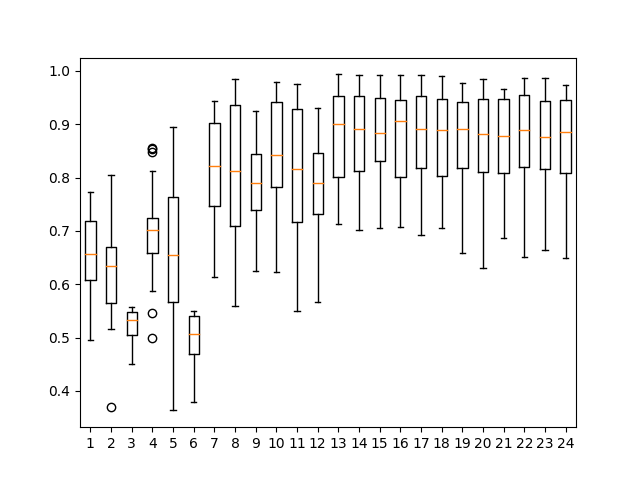
\includegraphics[scale=0.8]{acc_small_all.png}

\caption{\emph{Accuracy} + reducción de las variaciones de las metaheurísticas para los conjuntos pequeños}
\label{small-accu-all}
\end{figure}


\begin{figure}[h!]

	\centering
	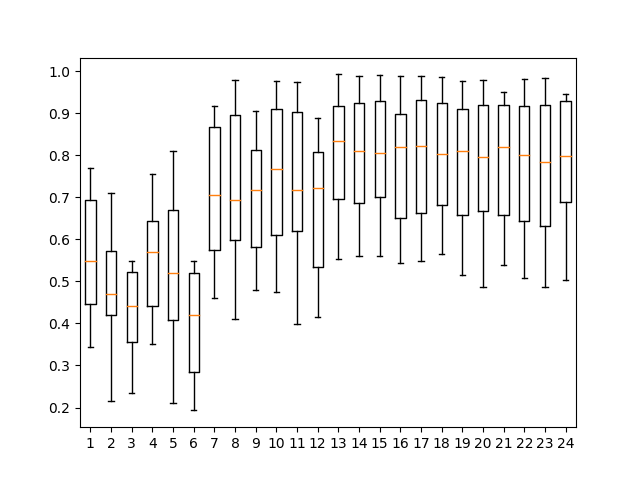
\includegraphics[scale=0.8]{kappa_small_all.png}

\caption{\emph{Kappa} + reducción de las variaciones de las metaheurísticas para los conjuntos pequeños}
\label{small-kap-all}
\end{figure}

Los \emph{boxplots} que van desde el número 13 hasta el 18 confirman que todas las variantes de MA presentan valores similares. Esto también sucede con CHC al ver los \emph{boxpĺots} que van desde el 19 hasta el 24. Los p-valores de las tablas \ref{wilcox-MA-peq} y \ref{wilcox-CHC-peq} en el anexo A muestran que todas las variantes son estadísticamente similares en \emph{accuracy} + reducción y \emph{kappa} + reducción.

De las figuras \ref{small-accu-all} y \ref{small-kap-all} también se puede apreciar que las variantes de MA y las de CHC presentan valores similares. Los resultados de la prueba \emph{Wilcoxon} (ver tabla \ref{wilcox-best-peq} en el anexo A) para MA y CHC muestran p-valores iguales a 6.934e-02 para \emph{accuracy} + reducción y 7.800e-02 para \emph{kappa} + reducción, lo que implica que ambos algoritmos son estadísticamente similares.

Como la diferencia entre MA y CHC es el tiempo de cómputo, se tiene que CHC con población inicial aleatoria presenta los tiempos más cortos y por lo tanto es la mejor metaheurística para resolver el problema de selección de prototipos sobre conjuntos pequeños.


\subsubsection{Conjuntos medianos}

En esta sección se estudia el comportamiento de las variaciones de GGA, SSGA, MA y CHC al resolver el problema de selección de instancias sobre conjuntos medianos. El objetivo es determinar cuál algoritmo presenta los mejores niveles de \emph{accuracy, kappa} y reducción. Además, se estudia el tiempo que requiere cada algoritmo en dar una solución, con lo que se busca evaluar si hay una buena relación entre tiempo y calidad de los resultados.


\begin{table}[h!]
\centering
\begin{tabular}{l c c c c c c}
\hline
\multirow{2}{*}{\textsc{Algoritmo}}
	& \multicolumn{2}{c}{\textsc{Accuracy}}
	& \multicolumn{2}{c}{\textsc{Kappa}}
	& \textsc{Reducción}
	& \textsc{Tiempo (seg)} \\
	& Training & Test
	& Training & Test \\ 
\hline
\hline

\textbf{GGA}         & \textbf{0.8702} & \textbf{0.7982} & \textbf{0.7375} & \textbf{0.5812} & \textbf{0.5641} & \textbf{110.0812} \\
CNN-GGA     & 0.7990 & 0.7051 & 0.5952 & 0.4426 & 0.7745 & 232.8342 \\
ENN-GGA     & 0.8475 & 0.8071 & 0.6949 & 0.5965 & 0.2862 & 125.8465 \\
RSS-GGA     & 0.8027 & 0.7520 & 0.5575 & 0.4547 & 0.6733 & 137.0381 \\
CNN-RSS-GGA & 0.8932 & 0.7890 & 0.7571 & 0.5516 & 0.5514 & 309.4603 \\
ENN-RSS-GGA & 0.9141 & 0.8155 & 0.8246 & 0.6168 & 0.1981 & 314.2968 \\

\hline

SSGA & 0.8431 & 0.8029 & 0.6676 & 0.5871 & 0.8392 & 3.5589 \\
CNN-SSGA & 0.8540 & 0.8007 & 0.6965 & 0.5923 & 0.8547 & 6.4410 \\
ENN-SSGA & 0.8200 & 0.8009 & 0.6324 & 0.5793 & 0.7459 & 5.6722 \\
\textbf{RSS-SSGA} & \textbf{0.8302} & \textbf{0.8045} & \textbf{0.6389} & \textbf{0.5854} & \textbf{0.8690} & \textbf{5.9946} \\
CNN-RSS-SSGA & 0.8586 & 0.8047 & 0.7043 & 0.5977 & 0.8121 & 10.5868 \\
ENN-RSS-SSGA & 0.8550 & 0.8078 & 0.7042 & 0.6004 & 0.7049 & 10.4293 \\

\hline

MA   & 0.8057 & 0.7908 & 0.5825 & 0.5564 & 0.9624 & 73.3461 \\
\textbf{CNN-MA} & \textbf{0.8116} & \textbf{0.8021} & \textbf{0.6000} & \textbf{0.5765} & \textbf{0.9572} & \textbf{57.3939} \\
ENN-MA & 0.7938 & 0.7925 & 0.5747 & 0.5608 & 0.9707 & 67.5310 \\
RSS-MA & 0.7924 & 0.7893 & 0.5611 & 0.5449 & 0.9671 & 69.5927 \\
CNN-RSS-MA & 0.8051 & 0.8015 & 0.5962 & 0.5808 & 0.9654 & 121.2220 \\
ENN-RSS-MA & 0.8070 & 0.7971 & 0.5886 & 0.5653 & 0.9633 & 112.0309 \\

\hline

\textbf{CHC} & \textbf{0.8313} & \textbf{0.8115} & \textbf{0.6347} & \textbf{0.5986} & \textbf{0.9455} & \textbf{2.8843} \\
CNN-CHC & 0.8303 & 0.8081 & 0.6337 & 0.5925 & 0.9352 & 4.6572 \\
ENN-CHC & 0.8107 & 0.8032 & 0.6084 & 0.5834 & 0.9356 & 5.0976 \\
RSS-CHC & 0.8151 & 0.8058 & 0.6074 & 0.5851 & 0.9535 & 4.7450 \\
CNN-RSS-CHC & 0.8276 & 0.8073 & 0.6280 & 0.5871 & 0.9319 & 6.7859 \\
ENN-RSS-CHC  & 0.8255 & 0.8074 & 0.6355 & 0.5944 & 0.9154 & 7.0284 \\


\hline
\end{tabular}
\caption{Promedios de las distintas variaciones de cada metaheurística para los conjuntos medianos}
\label{med-all}
\end{table}

Al estudiar los resultados obtenidos en la tabla \ref{med-all}, se pueden destacar los siguientes aspectos observados de las variaciones de GGA:

\begin{itemize}

\item GGA, ENN-GGA y ENN-RSS-GGA presentan los mejores niveles de \emph{accuracy y kappa}.

\item CNN-GGA presenta los niveles más bajos de \emph{accuracy}.

\item CNN-GGA y RSS-GGA presentan los niveles más bajos de \emph{kappa}. Al considerar que las otras variaciones obtienen un \emph{kappa} superior al 55\%, mientras que CNN-GGA y RSS-GGA obtienen valores por debajo del 46\%, se puede concluir que estas últimas tienen problemas para distinguir las clases minoritarias.

\item CNN-GGA presenta la tasa de reducción más alta con 77.45\%.

\item ENN-GGA y ENN-RSS-GGA presentan las tasas más bajas de reducción.

\item ENN-GGA y RSS-GGA son las variaciones, excluyendo a GGA, que menos tiempo toman en dar un resultado.

\end{itemize}

De las observaciones anteriores se puede concluir que GGA con población inicial aleatoria es la mejor variación de GGA; esto se debe a que presenta el mejor balance entre \emph{accuracy, kappa} y reducción, además de que es la variente más rápida. Cabe destacar CNN-GA porque presenta un \emph{accuracy} superior al 70\% a la vez que tiene la tasa de reducción más alta (21.04\% por encima de GGA); sin embargo, compromete los valores de \emph{kappa} (13.86\% por debajo de GGA) y tarda aproximadamente el doble de tiempo que GGA para dar una respuesta, razones que desfavorecen a CNN-GGA al momento de elegir una variante para resolver el problema de selección de prototipos.

Al pasar a los resultados obtenidos para las variaciones de SSGA, se puede observar:

\begin{itemize}

\item Todas las variaciones presentan niveles similares de \emph{accuracy}.

\item ENN-RSS-SSGA presenta el porcentaje más alto de \emph{kappa}, 1.33\% por encima de SSGA.

\item RSS-SSGA presenta la tasa de reducción más alta, 2.98\% por encima de SSGA.

\item Los mejores tiempos entre las variantes que usan heurísticas son los obtenidos por ENN-SSGA y RSS-SSGA. Ambas medidas se encuentran por debajo de los 7 segundos. 

\end{itemize}

Como los resultados entre las variaciones son muy similares, se necesita evaluar los p-valores de la prueba \emph{Wilcoxon}. En la tabla \ref{wilcox-SSGA-med} del apéndice A se puede apreciar que el p-valor de comparar RSS-SSGA con SSGA en \emph{accuracy} + reducción es de 7.013e-03, lo que implica que existe una diferencia estadística entre los dos algoritmos. Por lo tanto RSS-SSGA, que presenta la mayor tasa de reducción a la vez que mantiene buenos niveles de \emph{accuracy y kappa}, se puede considerar la mejor variación de SSGA.

Al evaluar los resultados obtenidos por las variaciones de MA, se observa:

\begin{itemize}

\item Todas las variaciones presentan valores similares de \emph{accuracy y kappa}.

\item Todas las variaciones presentan tasas de reducción similares.

\item CNN-MA es la variación que menos tarda en devolver un resultado entre todas, incluso tardando menos que CNN con población inicial aleatoria. Esto se debe a que con la población proporcionada por CNN se disminuyó el número de veces que MA utilizó el proceso de optimización interna.

\end{itemize}

Al revisar los resultados obtenidos por las variaciones de CHC, se observa:

\begin{itemize}

\item Todas las variaciones presentan valores similares de \emph{accuracy y kappa}.

\item CHC, CNN-CHC, ENN-CHC, RSS-CHC y CNN-RSS-CHC obtuvieron tasas de reducción similares. ENN-RSS-CHC, por su parte, obtuvo las tasas más bajas de reducción, estando 3.01\% por debajo de CHC. Esta diferencia es estadísticamente significativa al observar los resultados de los p-valores para reducción en la tabla \ref{wilcox-CHC-med} del anexo A.

\end{itemize}

De las observaciones anteriores se concluye que MA y CHC son metaheurísticas capaces de obtener resultados consistentes independientemente de la población inicial que utilicen. La decisión de cuales son las mejores variaciones depende del tiempo de cómputo: en el caso de MA, la mejor variación es CNN-MA; en el caso de CHC, CHC con población inicial aleatoria es la mejor.


Las figuras \ref{medium-accu-all} y \ref{medium-kap-all} muestran \emph{boxplots} de todas las variaciones de metaheurísticas para los conjuntos medianos, de izquierda a derecha los \emph{boxplots} representan las siguientes variaciones: '1':GGA, '2':CNN-GGA, '3':ENN-GGA, '4':RSS-GGA, '5':CNN-RSS-GGA, '6':ENN-RSS-GGA, '7':SSGA, '8':CNN-SSGA, '9':ENN-SSGA, '10':RSS-SSGA, '11':CNN-RSS-SSGA, '12':ENN-RSS-SSGA, '13':MA, '14':CNN-MA, '15':ENN-MA, '16':RSS-MA, '17':CNN-RSS-MA, '18':ENN-RSS-MA, '19':CHC, '20':CNN-CHC, '21':ENN-CHC, '22':RSS-CHC, '23':CNN-RSS-CHC y '24':ENN-RSS-CHC.

\begin{figure}[h!]

	\centering
	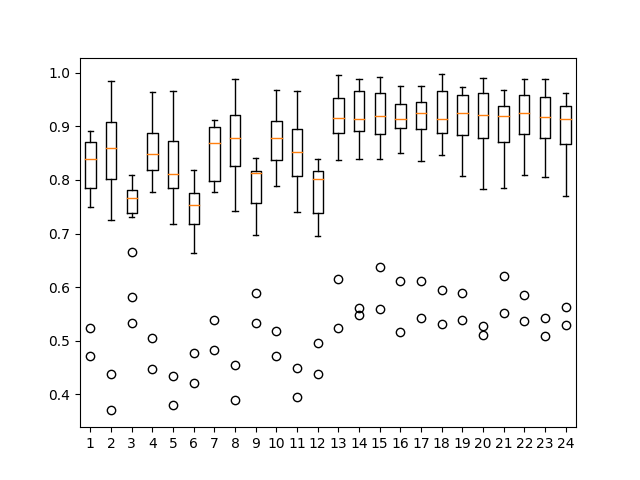
\includegraphics[scale=0.8]{acc_medium_all.png}

\caption{\emph{Accuracy} + reducción de las variaciones de las metaheurísticas para los conjuntos medianos}
\label{medium-accu-all}
\end{figure}


\begin{figure}[h!]

	\centering
	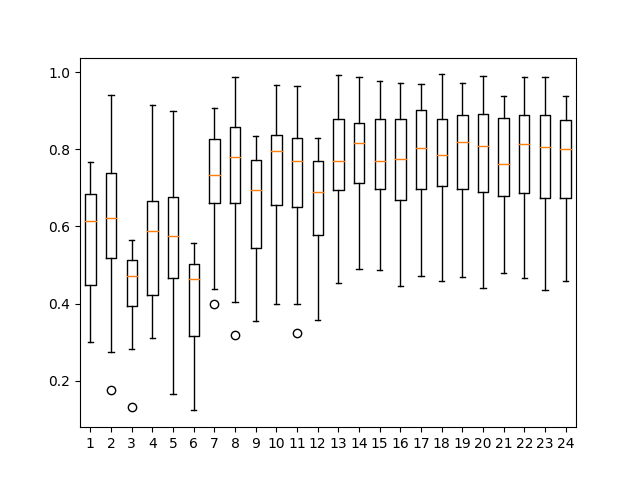
\includegraphics[scale=0.8]{kappa_medium_all.png}

\caption{\emph{Kappa} + reducción de las variaciones de las metaheurísticas para los conjuntos medianos}
\label{medium-kap-all}
\end{figure}

Los \emph{boxplots} que van desde el número 13 hasta el 18 confirman que todas las variantes de MA presentan valores similares. Los p-valores de la tabla \ref{wilcox-MA-med} en el anexo A muestran que todas las variantes de MA son estadísticamente similares en \emph{accuracy} + reducción y \emph{kappa} + reducción

Los \emph{boxpĺots} que van desde el 19 hasta el 24 muestran similitud entre las variantes de CHC. Al evaluar los p-valores de la tabla \ref{wilcox-CHC-med} del anexo A se tiene que CHC, CNN-CHC, ENN-CHC y RSS-CHC son estadísticamente similares, mientras que CNN-RSS-CHC y ENN-RSS-CHC son distintos al resto; esto es porque presentan niveles más bajo de reducción.

De las figuras \ref{small-accu-all} y \ref{small-kap-all} también se puede apreciar que las variantes de MA y las de CHC presentan valores similares. Los resultados de la prueba \emph{Wilcoxon} (ver tabla \ref{wilcox-best-med} en el anexo A) para CNN-MA y CHC muestran p-valores iguales a 6.292e-01 para \emph{accuracy} + reducción y 5.197e-01 para \emph{kappa} + reducción, lo que implica que ambos algoritmos son estadísticamente similares.

Como la diferencia entre CNN-MA y CHC es el tiempo de cómputo, se tiene que CHC con población inicial aleatoria presenta los tiempos más cortos y por lo tanto es la mejor metaheurística para resolver el problema de selección de prototipos sobre conjuntos medianos.


\subsubsection{Conjuntos Grandes}

En esta sección se estudia el comportamiento de las variaciones de GGA, SSGA, MA y CHC al resolver el problema de selección de instancias sobre conjuntos grandes. El objetivo es determinar cuál algoritmo presenta los mejores niveles de \emph{accuracy, kappa} y reducción. Además, se estudia el tiempo que requiere cada algoritmo en dar una solución, con lo que se busca evaluar si hay una buena relación entre tiempo y calidad de los resultados.

\begin{table}[h!]
\centering
\begin{tabular}{l c c c c c c}
\hline
\multirow{2}{*}{\textsc{Algoritmo}}
	& \multicolumn{2}{c}{\textsc{Accuracy}}
	& \multicolumn{2}{c}{\textsc{Kappa}}
	& \textsc{Reducción}
	& \textsc{Tiempo (seg)} \\
	& Training & Test
	& Training & Test \\ 
\hline
\hline

GGA         & 0.9316 & 0.8644 & 0.7994 & 0.6014 & 0.5050 & 672.0273 \\
CNN-GGA     & 0.7106 & 0.6431 & 0.4478 & 0.3094 & 0.8409 & 1568.8913 \\
ENN-GGA     & 0.9357 & 0.8890 & 0.7944 & 0.6453 & 0.1502 & 718.0400 \\
\textbf{RSS-GGA}     & \textbf{0.9150} & \textbf{0.8719} & \textbf{0.7227} & \textbf{0.5821} & \textbf{0.7083} & \textbf{1197.0505} \\
CNN-RSS-GGA & 0.9455 & 0.8588 & 0.8410 & 0.5885 & 0.6089 & 2646.6438 \\
ENN-RSS-GGA & 0.9574 & 0.8798 & 0.8669 & 0.6238 & 0.1025 & 1703.4263 \\

\hline

SSGA & 0.8911 & 0.8743 & 0.6953 & 0.6201 & 0.8056 & 27.6637 \\
CNN-SSGA & 0.8897 & 0.8512 & 0.7002 & 0.5939 & 0.8807 & 90.1004 \\
ENN-SSGA & 0.9097 & 0.8892 & 0.7113 & 0.6441 & 0.6823 & 34.9024 \\
\textbf{RSS-SSGA} & \textbf{0.8968} & \textbf{0.8826} & \textbf{0.6743} & \textbf{0.6271} & \textbf{0.8927} & \textbf{57.7995} \\
CNN-RSS-SSGA & 0.9002 & 0.8634 & 0.7140 & 0.6069 & 0.8434 & 99.1629 \\
ENN-RSS-SSGA & 0.9112 & 0.8805 & 0.7245 & 0.6272 & 0.6668 & 78.5967 \\

\hline

\textbf{MA}   & \textbf{0.8904} & \textbf{0.8999} & \textbf{0.6499} & \textbf{0.6510} & \textbf{0.9973} & \textbf{256.1432} \\
CNN-MA & 0.8925 & 0.8926 & 0.6360 & 0.6341 & 0.9884 & 612.7902 \\
ENN-MA & 0.8807 & 0.8902 & 0.6072 & 0.6145 & 0.9976 & 288.6525 \\
RSS-MA & 0.9000 & 0.9002 & 0.6347 & 0.6343 & 0.9746 & 527.9115 \\
CNN-RSS-MA & 0.8857 & 0.8951 & 0.6176 & 0.6160 & 0.9707 & 960.3951 \\
ENN-RSS-MA & 0.8746 & 0.8912 & 0.6292 & 0.6386 & 0.9969 & 443.0003 \\

\hline

\textbf{CHC}  & \textbf{0.8961} & \textbf{0.8934} & \textbf{0.6614} & \textbf{0.6506} & \textbf{0.9615} & \textbf{16.8665} \\
CNN-CHC & 0.8903 & 0.8871 & 0.6554 & 0.6437 & 0.9771 & 38.3314 \\
ENN-CHC & 0.8993 & 0.8964 & 0.6746 & 0.6631 & 0.9233 & 27.3520 \\
RSS-CHC & 0.8972 & 0.8962 & 0.6591 & 0.6526 & 0.9819 & 41.1142 \\
CNN-RSS-CHC & 0.8945 & 0.8910 & 0.8945 & 0.6435 & 0.9719 & 50.5800 \\
ENN-RSS-CHC & 0.8975 & 0.8922 & 0.6721 & 0.6532 & 0.9099 & 47.4006 \\

\hline
\end{tabular}
\caption{Promedios de las distintas variaciones de cada metaheurística para los conjuntos grandes}
\label{grande-all}
\end{table}

Al estudiar los resultados obtenidos en la tabla \ref{grande-all}, se pueden destacar los siguientes aspectos observados de las variaciones de GGA:

\begin{itemize}

\item RSS-GGA, ENN-GGA y ENN-RSS-GGA presentan los mejores niveles de \emph{accuracy}. 

\item ENN-GGA y ENN-RSS-GGA presentan los mejores niveles de \emph{kappa}.

\item CNN-GGA presenta los peores porcentajes de \emph{accuracy y kappa}. 

\item CNN-GGA y RSS-GGA presentan las mejores tasas de reducción.

\item ENN-GGA y ENN-RSS-GGA presentan las peores tasas de reducción.

\item ENN-GGA y RSS-GGA son las variaciones, excluyendo a GGA, que menos tiempo toman en dar un resultado.

\end{itemize}

De las observaciones anteriores se puede concluir que RSS-GGA es la mejor variación de GGA; esto se debe a que presenta el mejor balance entre \emph{accuracy, kappa} y reducción. Cabe destacar que RSS-GGA obtiene una tasa de reducción 20.33\% mayor que GGA sin comprometer sus niveles de \emph{accuracy y kappa}, lo cual justifica el costo adicional de tiempo que conlleva utilizar RSS.

Al pasar a los resultados obtenidos para las variaciones de SSGA, se puede observar:

\begin{itemize}

\item RSS-SSGA, ENN-SSGA y ENN-RSS-SSGA presentan los mejores valores para \emph{accuracy y kappa}.

\item RSS-SSGA y CNN-SSGA presentan las tasas de reducción más alta.

\item Los mejores tiempos entre las variantes que usan heurísticas son los obtenidos por ENN-SSGA y RSS-SSGA. Ambas variaciones presentan tiempos por debajo del minuto.

\end{itemize}

De las consideraciones anteriores, se puede concluir que RSS-SSGA es la mejor variación de SSGA, ya que presenta la mayor tasa de reducción: 8.71\% por encima de SSGA con población inicial aleatoria, a la vez que mantiene buenos niveles de \emph{accuracy y kappa}, razones que justifican el tiempo adicional de cómputo.

Al evaluar los resultados obtenidos por las variaciones de MA y CHC, se observa:

\begin{itemize}

\item Todas las variaciones presentan valores similares de \emph{accuracy y kappa}.

\item Todas las variaciones presentan tasas de reducción similares.

\end{itemize}

De las observaciones anteriores se concluye que MA y CHC son metaheurísticas capaces de obtener resultados consistentes independientemente de la población inicial que utilicen. Por lo tanto el uso de heurísticas no conlleva a un beneficio real y sólo aumenta el tiempo de cómputo, razón por la cual MA y CHC con población incial aleatoria son las mejores varientes de sus respectivas metaheurísticas.

Al comparar todas las metaheurísticas, se tiene que las variantes de MA y CHC presentan los mejores valores en \emph{accuracy, kappa} y reducción. Al contrastar MA con CHC se tiene que presentan valores de \emph{accuracy y kappa} muy similares, la diferencia está en la tasa de reducción, donde MA supera en 3.58\% a CHC. Sin embargo, si se toma en cuenta que MA tarda 15 veces más en regresar un resultado y que CHC es la metaheurística más rápida; se puede concluir que CHC es la mejor metaheurística para resolver el problema de selección de prototipos sobre conjuntos grandes.
%\chapter{Capítulo4}
\label{capitulo4}
\lhead{Capítulo 4. \emph{Capítulo 4}}

Capítulo 4


% +--------------+
% | CONCLUSIONES |
% +--------------+
\chapter*{Conclusiones y Recomendaciones}
\label{conclusiones}
\lhead{\emph{Conclusiones y Recomendaciones}}
\addcontentsline{toc}{chapter}{Conclusiones y Recomendaciones}

El presente trabajo de investigación implementó tres heurísticas y cuatro metahuerísticas con el fin de evaluar si la utilización de las heurísticas como métodos de inicialización de la población de las metaheurísticas mejora el \emph{accuracy, kappa} y la tasa de reducción de las mismas en comparación con una inicialización aleatoria de la población. Además, se buscó determinar cuales son las mejores combinaciones de heurísticas y metaheurísticas al evaluarse bajo las métricas antes mencionadas.

Para lograr este cometido, se probaron todas las combinaciones posibles sobre conjuntos de datos pequeños, medianos y grandes. Es por ello que se usó el proceso de estratificación propuesto por \emph{Cano, J. et al.} en \cite{cano2005stratification} para reducir los tiempos de cómputo de los conjuntos medianos y grandes. Por otra parte, se usó una herramienta de entonación conocida como \emph{Irace} para conseguir los mejores parámetros para las distintas metaheurísticas.

De los resultados obtenidos se observa que la utilización de heurísticas no conllevan en una mejoría significativa. En el caso de GGA, el uso de heurísticas desbalancea la relación entre \emph{accuracy, kappa} y reducción, esto se aprecia cuando cada algoritmo favorece una métrica sobre la otra. En el caso de MA y CHC se observan resultados similares entre todas las variaciones, lo que reafirma el hecho de que ambas metaheurísticas consiguen soluciones parecidas de manera consistente, independientemente de la población inicial. Sólo SSGA se benefició del uso de heurísticas, ya que obtuvo mejores tasas de reducción con RSS, aumentando en promedio 5.65\% sobre lo obtenido por SSGA con población inicial aleatoria

Cuando se comparan todas las metaheurísticas, se tiene que las variantes de CHC y MA presentan los mejores valores de \emph{accuracy, kappa} y reducción para los conjuntos de los tres tamaños, además, estas metaheurísticas son estadísticamente similares; por lo tanto, se elige CHC con población inicial aleatoria como la mejor opción para resolver el problema de selección de prototipos para los conjuntos de los tres tamaños, porque es la metaheurística más rápida en devolver un resultado. 

Las recomendaciones que se desprenden de esta investigación incluyen: 

\begin{itemize}

\item Probar otras heurísticas y metaheurísticas a las utilizadas en este trabajo.

\item Utilizar otras funciones de distancia distintas a la euclídea con el fin de incorporar conjuntos de datos categóricos.

\item Plantear el problema de selección de prototipos como un problema de optimización multiobjetivo en relación al \emph{accuracy, kappa}, reducción y tiempo par estudiar el comportamiento de los distintos algoritmos frente a la curva pareto obtenida.

\item Prbar herramientas de entonación distintas a \emph{Irace} para evaluar el impacto de los párametros sobre la obtención de resultados.

\end{itemize}



% +--------------+
% | BIBLIOGRAFIA |
% +--------------+
\cleardoublepage
\clearpage
\phantomsection
\label{Bibliography}
\addcontentsline{toc}{chapter}{Bibliografía}
\lhead{\emph{Bibliografía}}
\bibliography{bibliografia}
\bibliographystyle{alpha}
\addtocontents{toc}{\vspace{2em}}

% +-----------+
% | APENDICES |
% +-----------+
\appendix
\chapter{Entonación de las metaheurísticas}
\label{Apéndices}
\lhead{Apéndice A. \emph{Apéndice A}}

Para la entonación de las metaheurísticas se usó \emph{irace} \cite{lopez2016irace}, el cual es un paquete de R que implementa el método de entonación automática conocido como \emph{iterated F-race}. La esencia de \emph{iterated F-race}
es hacer varias carreras, las cuales son procesos internos del algoritmo que ponen a competir un conjunto de vectores de parámetros (también conocidos como configuraciones) con un repertorio de problemas, con el fin de recopilar datos referentes al desempeño de cada configuración para hacer pruebas estadísticas que determinan cuáles son las mejores y además, descartar las peores en una etapa temprana de la carrera. 

\emph{Iterated F-race} trata de un método que consiste en tres pasos: (1) elegir varias configuraciones posibles de acuerdo a una distribución en particular y así formar una población, (2) elegir una población de configuraciones (3) actualizar la distribución de la población de tal manera que sea sesgada a favor de las mejores configuraciones. Estos tres pasos son repetidos hasta que pase un número de iteraciones dadas por el usuario. El algoritmo de \emph{iterated F-race} se presenta en \ref{irace}.

\begin{algorithm}
\caption{IRACE}
\label{irace}
\begin{algorithmic}[1]

\Require{\texttt{I} conjunto de instancias del problema a entonar, \texttt{X} espacio de configuraciones, U función de utilidad, \texttt{B} número de iteraciones con el que se cuenta}
\Ensure{$\theta^{elite}$ mejores configuraciones encontradas}

\State $\theta_1 \gets$ una muestra uniforme de X
\State $\theta^{elite} \gets$ resultado de una \textbf{carrera} al usar $\theta_1$ como población y con número de iteraciones $B_1$
\State $j \gets 1$
\While{$B^{usado} \leq B$}
	\State $j \gets j + 1$
	\State $\theta^{nueva} \gets$ muestra sesgada hacia $\theta^{elite}$ de X 
	\State $\theta_j \gets \theta^{nueva} \cup \theta^{elite}$
	\State $\theta^{elite} \gets$ resultado de una \textbf{carrera} al usar $\theta_j$ como población y con número de iteraciones $B_j$
\EndWhile
\State \Return $\theta^{elite}$

\end{algorithmic}
\end{algorithm}

%\emph{Irace} empieza estimando cuántas iteraciones $N^{iter}$ va a ejecutar; este valor está en función al número de parámetros que se piensa entonar, por lo tanto $N^{iter} = \lfloor 2 + log_2 N^{parametros} \rfloor$, donde $N^{parametros}$ representa el número de parámetros, con la idea de que mientras más parámetros se necesite entonar, mayor será la cantidad de iteraciones que una carrera en específico necesita para conseguir las configuraciones élites. El cálculo de cuántas carreras se van a realizar en total, calculado $N^{iter}$, va en función de cuanto presupuesto B se le asigne a todo el proceso; se calcula la cantidad de carreras como $\lfloor B / N^{iter} \rfloor$. Si la cantidad de carreras es 0 entonces \emph{irace} pide que se introduzca un B mayor. Para este estudio, se asignó para los conjuntos pequeños y medianos $ B = 1000$ iteraciones y en cada carrera las metaheurísticas disponían de 1000 iteraciones para hallar el mejor valor posible; en cambio, para los conjuntos grandes se asignó $B = 400$ y cada metaherística en cada carrera disponía de 300 iteraciones.

Cabe acotar que \emph{irace} asume que el problema sobre el cual se va a entonar es un problema de minimización. Por lo tanto, siempre se busca menores valores de la función de utilidad U para cada configuración; además, luego de cada carrera asigna un rango $r_z$ dependiendo de cómo se compare la configuración z con respecto al resto, a menor rango, mejor es la configuración; por lo tanto, el conjunto de élites $\theta^{elite}$ está conformado por los $k$ elementos con menor rango. El número $k$ es calculado al principio de la corrida de \emph{irace} y en este trabajo se deja su cálculo automático por defecto.

%Por otra parte,en la primera línea del algoritmo \ref{irace}, se hace un muestreo uniforme del espacio de configuraciones X con una distribución normal truncada. En las siguientes iteraciones se va sesgando el muestreo con las configuraciones élites encontradas en la línea 6, esto se logra usando una probabilidad $p_z$ con la cual se toma una configuración $ \theta^z$ que se calcula como en la ecuación (2.5), donde $N^{elite}_{j-1}$ es el número de élites de la iteración j-1:

%\begin{equation}
%p_z = \frac{N^{elite}_{j-1} - r_z + 1}{N^{elite}_{j-1}*\frac{N^{elite}_{j-1}+1}{2}}
%\end{equation} 

%Una vez obtenido un $\theta^z$ se genera una nueva configuración tomando una muestra del espacio de parámetros X, un parámetro d a la vez de entre un rango $[d_{inf},d^{sup}]$ definido por el usuario, usando una distribución normal truncada $\mathcal{N}(\mu^z_d,(\sigma^j_d)^2)$ donde $\mu^z_d$, que representa la media, es el valor $\theta^z_d$ y la variancia $\sigma^j_d$ está definida como $(d^{sup}-d_{inf}) / 2 $ en la iteración j, con una actualización progresiva  en cada iteración dada por la ecuación (2.6), donde $N^{nuevo}_j$ es el número de configuraciones en la población que se va a generar en la línea 6 del algoritmo \ref{irace} en la iteración j, con el fin de acercar cada vez más los nuevos elementos a la élite encontrada en las últimas iteraciones del experimento.

%\begin{equation}
%\sigma^j_d = \sigma^{j-1}_d *\left(\frac{1}{N^{nuevo}_j}\right)^{\frac{1}{N^{parametros}}}
%\end{equation}

%El proceso de carrera (\emph{racing} en inglés) para la entonación de metaheurísticas con el cual se realiza el paso (2) (líneas 2 y 8), fue propuesto por \emph{Birattari, M. et al.} en \cite{birattari2002racing}. La carrera empieza usando una población con configuraciones; luego, a cada iteración de la carrera, las configuraciones son evaluadas en una sola instancia $I_j$. Después de un número iteraciones dadas por un parámetro T, aquellas configuraciones que estadísticamente tienen un desempeño inferior al resto son descartadas. \emph{Irace} establece  $T = 1$; además, puede usar una prueba Friedman no paramétrica o una prueba t-test como prueba estadística para hacer las comparaciones entre las configuraciones. Por recomendación de los autores, se usa una prueba t-test con un valor de significancia de 0.05 ya que, según sus criterios, es la más adecuada para la entonación de parámetros de valores continuos.

La prueba estadística utilizada por la carrera para reemplazar las peores configuraciones y preservar las élites es la prueba \emph{Friedman} no paramétrica o la prueba \emph{t-test}. Por recomendación de los autores se usa una prueba \emph{t-test} con un valor de significancia de 0.05 ya que, según sus criterios, es la más adecuada para la entonación de parámetros de valores continuos.

\emph{Irace}, además, implementa un método de reinicialización cuando la población de configuraciones converge prematuramente. En este proceso se mantienen las configuraciones élites de la última carrera y empieza de nuevo segun ciertas consideraciones. Aunado a esto, \emph{irace} también implementa un sistema de carrera elitista, el cual evita que las mejores configuraciones encontradas hasta el momento se pierdan en una carrera producto de una serie desfavorable de evaluaciones en un momento dado. En este trabajo se usa tanto el método de reinicialización como el sistema de carrera elitista. Para más información de todas las funciones y utilidades que presenta esta herramemienta, se recomienda leer \cite{lopez2016irace}.

\chapter{Pruebas por pares \emph{Wilcoxon}}
\label{Apéndices}
\lhead{Apéndice B. \emph{Apéndice B}}

\begin{table}[h!]
\centering
\begin{adjustbox}{max width =\textwidth}
\begin{tabular}{l c c c c c}
\hline
	\textsc{Algoritmo}
	& \multicolumn{1}{c}{\textsc{Accuracy}}
	& \multicolumn{1}{c}{\textsc{Kappa}}
	& \multicolumn{1}{c}{\textsc{Reducción}} 
	& \multicolumn{1}{c}{\textsc{Accuracy + reducción}} 
	& \multicolumn{1}{c}{\textsc{kappa + reducción}} \\
\hline
\hline

 & p-valor & p-valor & p-valor & p-valor & p-valor \\

GGA \\
vsSSGA & 3.822e-03 & 8.905e-04 & 1.569e-05 & 1.389e-05 & 2.257e-05 \\ 
vsMA & 3.507e-03 & 2.064e-03 & 1.229e-05 & 1.229e-05 & 1.229e-05 \\ 
vsCHC & 3.822e-03 & 8.084e-04 & 1.228e-05 & 1.228e-05 & 1.229e-05 \\

\hline

SSGA \\
vsMA & 1.373e-01 & 1.615e-01 & 1.229e-05 & 1.229e-05 & 2.543e-05 \\
vsCHC & 1.779e-01 & 3.395e-01 & 1.228e-05 & 1.229e-05 & 2.001e-05 \\

\hline

MA \\
vsCHC & 1.873e-01 & 1.425e-01 & 8.401e-01 & 6.934e-02 & 7.800e-02 \\ 

\hline

\end{tabular}
\end{adjustbox}
\caption[Pruebas de \emph{Wilcoxon} entre las metaheurísticas para conjuntos pequeños]{$p$-valor de pruebas de rangos con signo de \emph{Wilcoxon} para las distintas metaheurísticas sobre conjuntos pequeños}
\label{wilcox-meta-peq}
\end{table}

\begin{table}[h!]
\centering
\begin{adjustbox}{max width =\textwidth}
\begin{tabular}{l c c c c c}
\hline
	\textsc{Algoritmo}
	& \multicolumn{1}{c}{\textsc{Accuracy}}
	& \multicolumn{1}{c}{\textsc{Kappa}}
	& \multicolumn{1}{c}{\textsc{Reducción}} 
	& \multicolumn{1}{c}{\textsc{Accuracy + reducción}} 
	& \multicolumn{1}{c}{\textsc{kappa + reducción}} \\
\hline
\hline

 & p-valor & p-valor & p-valor & p-valor & p-valor \\

GGA \\
vsSSGA & 1.754e-02 & 1.262e-01 & 1.316e-04 & 1.316e-04 & 1.316e-04 \\ 
vsMA & 6.874e-01 & 2.432e-01 & 1.318e-04 & 1.318e-04 & 1.318e-04 \\
vsCHC & 2.977e-02 & 4.445e-01 & 1.318e-04 & 1.318e-04 & 1.318e-04 \\ 

\hline

SSGA \\
vsMA & 1.842e-01 & 1.365e-01 & 1.318e-04 & 1.318e-04 & 1.318e-04 \\
vsCHC & 2.122e-01 & 4.939e-01 & 1.316e-04 & 1.318e-04 & 1.316e-04 \\

\hline

MA \\
vsCHC & 1.57e-02 & 5.338e-02 & 9.100e-02 & 6.009e-01 & 7.172e-01 \\ 

\hline


\end{tabular}
\end{adjustbox}
\caption[Pruebas de \emph{Wilcoxon} entre las metaheurísticas para conjuntos pequeños]{$p$-valor de pruebas de rangos con signo de \emph{Wilcoxon} para las distintas metaheurísticas sobre conjuntos medianos}
\label{wilcox-meta-med}
\end{table}

\begin{table}[h!]
\centering
\begin{adjustbox}{max width =\textwidth}
\begin{tabular}{l c c c c c}
\hline
	\textsc{Algoritmo}
	& \multicolumn{1}{c}{\textsc{Accuracy}}
	& \multicolumn{1}{c}{\textsc{Kappa}}
	& \multicolumn{1}{c}{\textsc{Reducción}} 
	& \multicolumn{1}{c}{\textsc{Accuracy + reducción}} 
	& \multicolumn{1}{c}{\textsc{kappa + reducción}} \\
\hline
\hline

 & p-valor & p-valor & p-valor & p-valor & p-valor \\

GGA\\
vsCNN-GGA  & 6.329e-02 & 2.641e-01 & 2.209e-01 & 6.186e-01 & 8.612e-01 \\   
vsENN-GGA  & 7.237e-03 & 2.964e-03 & 1.229e-05 & 3.624e-05 & 1.010e-04 \\  
vsRSS-GGA  & 1.425e-01 & 2.528e-01 & 1.571e-05 & 1.128e-04 & 2.062e-03 \\    
vsCNN-RSS-GGA & 4.926e-01 & 7.570e-01 & 8.191e-01 & 9.036e-01 & 9.036e-01 \\
vsENN-RSS-GGA & 1.721e-03 & 9.804e-04 & 1.229e-05 & 1.229e-05 & 1.228e-05 \\

\hline

CNN-GGA\\
vsENN-GGA & 1.078e-03 & 1.100e-02 & 6.451e-05 & 1.186e-03 & 1.330e-02 \\
vsRSS-GGA & 3.606e-01 & 9.893e-01 & 2.541e-05 & 4.458e-04 & 6.313e-03 \\
vsCNN-RSS-GGA & 3.327e-01 & 5.629e-01 & 5.129e-05 & 1.186e-01 & 3.674e-01 \\ 
vsENN-RSS-GGA & 2.038e-04 & 2.064e-03 & 1.390e-05 & 2.257e-05 & 2.958e-04 \\ 

\hline

ENN-GGA\\
vsRSS-GGA & 5.448e-04 & 2.064e-03 & 1.229e-05 & 1.229e-05 & 1.566e-04 \\ 
vsCNN-RSS-GGA & 3.820e-03 & 4.797e-02 & 2.665e-04 & 1.800e-03 & 2.466e-02 \\
vsENN-RSS-GGA & 8.791e-01 & 8.864e-01 & 3.839e-05 & 1.244e-03 & 1.855e-02 \\ 

\hline

RSS-GGA\\
vsCNN-RSS-GGA & 8.192e-01 & 5.677e-01 & 1.229e-05 & 2.665e-04 & 5.816e-03 \\
vsENN-RSS-GGA  & 1.744e-04 & 4.028e-04 & 1.229e-05 & 1.389e-05 & 2.543e-05 \\

\hline

CNN-RSS-GGA\\
vsENN-RSS-GGA & 1.017e-03 & 6.313e-03 & 1.773e-05 & 2.001e-05 & 6.451e-05 \\ 
 
\hline

\end{tabular}
\end{adjustbox}
\caption[Pruebas de \emph{Wilcoxon} entre GGA y variaciones para conjuntos pequeños]{$p$-valor de pruebas de rangos con signo de \emph{Wilcoxon} para GGA sobre conjuntos pequeños}
\label{wilcox-gga-peq}
\end{table}

\begin{table}[h!]
\centering
\begin{adjustbox}{max width =\textwidth}
\begin{tabular}{l c c c c c}
\hline
	\textsc{Algoritmo}
	& \multicolumn{1}{c}{\textsc{Accuracy}}
	& \multicolumn{1}{c}{\textsc{Kappa}}
	& \multicolumn{1}{c}{\textsc{Reducción}} 
	& \multicolumn{1}{c}{\textsc{Accuracy + reducción}} 
	& \multicolumn{1}{c}{\textsc{kappa + reducción}} \\

\hline
\hline

 & p-valor & p-valor & p-valor & p-valor & p-valor \\

SSGA\\
vsCNN-SSGA  & 2.758e-01 & 1.578e-01 & 9.250e-01 & 6.964e-01 & 5.098e-01 \\    
vsENN-SSGA   & 5.203e-02 & 1.873e-01 & 1.390e-05 & 4.028e-04 & 2.259e-03 \\ 
vsRSS-SSGA     & 7.533e-01 & 9.893e-01 & 2.001e-05 & 8.905e-04 & 3.822e-03 \\
vsCNN-RSS-SSGA & 5.812e-01 & 8.191e-01 & 5.812e-01 & 6.571e-01 & 9.678e-01 \\
vsENN-RSS-SSGA & 2.414e-01 & 1.451e-01 & 1.229e-05 & 2.257e-05 & 8.905e-04 \\

\hline

CNN-SSGA\\
vsENN-SSGA & 1.603e-02 & 4.501e-02 & 3.822e-03 & 9.526e-02 & 2.528e-01 \\ 
vsRSS-SSGA & 5.774e-01 & 5.998e-01 & 2.692e-05 & 1.186e-03 & 1.430e-03 \\
vsCNN-RSS-SSGA & 2.418e-01 & 4.797e-02 & 5.933e-02 & 9.464e-01 & 1.658e-01 \\
vsENN-RSS-SSGA & 4.550e-02 & 2.227e-02 & 4.574e-05 & 1.303e-03 & 1.994e-02 \\

\hline

ENN-SSGA\\
vsRSS-SSGA & 4.501e-02 & 1.155e-01 & 1.773e-05 & 1.405e-04 & 9.804e-04 \\
vsCNN-RSS-SSGA & 1.725e-02 & 2.109e-01 & 4.676e-03 & 7.356e-02 & 9.797e-02 \\
vsENN-RSS-SSGA & 2.840e-01 & 5.998e-01 & 4.559e-05 & 8.038e-03 & 6.148e-02 \\ 

\hline

RSS-SSGA\\
vsCNN-RSS-SSGA & 6.476e-01 & 4.073e-01 & 1.229e-05 & 8.085e-05 & 2.699e-03 \\
vsENN-RSS-SSGA  & 4.548e-02 & 4.797e-02 & 1.229e-05 & 1.773e-05 & 9.042e-05 \\ 

\hline

CNN-RSS-SSGA\\
vsENN-RSS-SSGA & 5.437e-02 & 1.218e-01 & 3.223e-05 & 2.159e-04 & 7.329e-04 \\

\hline 

\end{tabular}
\end{adjustbox}
\caption[Pruebas de \emph{Wilcoxon} entre SSGA y variaciones para conjuntos pequeños]{$p$-valor de pruebas de rangos con signo de \emph{Wilcoxon} para SSGA sobre conjuntos pequeños}
\label{wilcox-SSGA-peq}
\end{table}

\begin{table}[h!]
\centering
\begin{adjustbox}{max width =\textwidth}
\begin{tabular}{l c c c c c}
\hline
	\textsc{Algoritmo}
	& \multicolumn{1}{c}{\textsc{Accuracy}}
	& \multicolumn{1}{c}{\textsc{Kappa}}
	& \multicolumn{1}{c}{\textsc{Reducción}} 
	& \multicolumn{1}{c}{\textsc{Accuracy + reducción}} 
	& \multicolumn{1}{c}{\textsc{kappa + reducción}} \\

\hline
\hline

 & p-valor & p-valor & p-valor & p-valor & p-valor \\

MA\\
vsCNN-MA     & 6.682e-01 & 6.892e-01 & 1.430e-03 & 6.668e-01 & 9.678e-01 \\ 
vsENN-MA     & 9.678e-01 & 9.036e-01 & 1.617e-01 & 5.629e-01 & 9.036e-01 \\
vsRSS-MA     & 1.035e-01 & 1.094e-01 & 2.469e-03 & 4.432e-01 & 2.418e-01 \\ 
vsCNN-RSS-MA & 1.353e-01 & 6.934e-02 & 6.932e-02 & 4.215e-02 & 3.704e-02 \\ 
vsENN-RSS-MA & 6.034e-01 & 3.967e-01 & 3.404e-03 & 3.002e-01 & 6.766e-01 \\

\hline

CNN-MA\\
vsENN-MA & 1.918e-01 & 4.118e-01 & 1.261e-01 & 7.751e-01 & 9.893e-01 \\ 
vsRSS-MA & 2.227e-02 & 1.516e-02 & 4.073e-05 & 5.449e-01 & 1.155e-01 \\ 
vsCNN-RSS-MA & 8.571e-03 & 2.299e-02 & 2.879e-01 & 3.243e-02 & 2.831e-02 \\ 
vsENN-RSS-MA & 3.819e-01 & 5.629e-01 & 3.129e-01 & 3.194e-01 & 3.819e-01 \\ 

\hline

ENN-MA\\
vsRSS-MA & 2.209e-01 & 1.919e-01 & 2.956e-04 & 9.036e-01 & 5.449e-01 \\ 
vsCNN-RSS-MA & 1.742e-01 & 3.129e-01 & 6.265e-01 & 1.855e-02 & 1.155e-01 \\ 
vsENN-RSS-MA & 9.464e-01 & 6.964e-01 & 1.479e-03 & 2.641e-01 & 8.401e-01 \\ 

\hline

RSS-MA\\
vsCNN-RSS-MA & 4.576e-01 & 2.478e-01 & 1.822e-05 & 3.458e-01 & 8.415e-01 \\
vsENN-RSS-MA & 6.746e-02 & 3.955e-02 & 3.220e-05 & 7.982e-01 & 3.674e-01 \\ 

\hline

CNN-RSS-MA\\
vsENN-RSS-MA & 3.002e-01 & 1.829e-01 & 1.793e-01 & 9.250e-01 & 3.674e-01 \\ 

\hline 

\end{tabular}
\end{adjustbox}
\caption[Pruebas de \emph{Wilcoxon} entre MA y variaciones para conjuntos pequeños]{$p$-valor de pruebas de rangos con signo de \emph{Wilcoxon} para MA sobre conjuntos pequeños}
\label{wilcox-MA-peq}
\end{table}


\begin{table}[h!]
\centering
\begin{adjustbox}{max width =\textwidth}
\begin{tabular}{l c c c c c}
\hline
	\textsc{Algoritmo}
	& \multicolumn{1}{c}{\textsc{Accuracy}}
	& \multicolumn{1}{c}{\textsc{Kappa}}
	& \multicolumn{1}{c}{\textsc{Reducción}} 
	& \multicolumn{1}{c}{\textsc{Accuracy + reducción}} 
	& \multicolumn{1}{c}{\textsc{kappa + reducción}} \\
\hline
\hline

 & p-valor & p-valor & p-valor & p-valor & p-valor \\

CHC\\
vsCNN-CHC     & 3.967e-01 & 4.432e-01 & 1.188e-02 & 1.658e-01 & 1.742e-01 \\ 
vsENN-CHC     & 8.823e-01 & 8.506e-01 & 4.245e-02 & 3.674e-01 & 4.593e-01 \\ 
vsRSS-CHC     & 5.629e-01 & 3.533e-01 & 6.642e-03 & 7.982e-01 & 6.571e-01 \\ 
vsCNN-RSS-CHC & 3.674e-01 & 1.284e-01 & 2.699e-01 & 4.593e-01 & 2.528e-01 \\ 
vsENN-RSS-CHC & 8.639e-01 & 9.464e-01 & 6.739e-04 & 9.797e-02 & 2.109e-01 \\ 

\hline

CNN-CHC\\
vsENN-CHC & 2.418e-01 & 3.395e-01 & 8.823e-01 & 6.571e-01 & 5.812e-01 \\
vsRSS-CHC & 9.515e-01 & 4.118e-01 & 9.067e-05 & 1.658e-01 & 9.893e-01 \\
vsCNN-RSS-CHC & 9.886e-01 & 3.606e-01 & 2.418e-01 & 7.164e-01 & 8.191e-01 \\ 
vsENN-RSS-CHC & 3.615e-01 & 5.633e-01 & 2.528e-01 & 9.036e-01 & 7.982e-01 \\ 

\hline

ENN-CHC\\
vsRSS-CHC & 4.432e-01 & 3.260e-01 & 1.498e-03 & 4.273e-01 & 9.464e-01 \\ 
vsCNN-RSS-CHC & 5.098e-01 & 3.002e-01 & 6.766e-01 & 9.893e-01 & 5.449e-01 \\ 
vsENN-RSS-CHC & 6.682e-01 & 3.819e-01 & 2.380e-02 & 2.109e-01 & 1.285e-01 \\ 

\hline

RSS-CHC\\
vsCNN-RSS-CHC & 7.672e-01 & 6.186e-01 & 1.756e-03 & 6.092e-01 & 9.464e-01 \\ 
vsENN-RSS-CHC & 4.405e-01 & 3.819e-01 & 1.127e-04 & 2.418e-01 & 7.366e-01 \\ 

\hline

CNN-RSS-CHC\\
vsENN-RSS-CHC & 7.317e-01 & 6.071e-01 & 1.913e-02 & 6.186e-01 & 6.766e-01 \\ 

\hline 

\end{tabular}
\end{adjustbox}
\caption[Pruebas de \emph{Wilcoxon} entre CHC y variaciones para conjuntos pequeños]{$p$-valor de pruebas de rangos con signo de \emph{Wilcoxon} para CHC sobre conjuntos pequeños}
\label{wilcox-CHC-peq}
\end{table}


\begin{table}[h!]
\centering
\begin{adjustbox}{max width =\textwidth}
\begin{tabular}{l c c c c c}
\hline
	\textsc{Algoritmo}
	& \multicolumn{1}{c}{\textsc{Accuracy}}
	& \multicolumn{1}{c}{\textsc{Kappa}}
	& \multicolumn{1}{c}{\textsc{Reducción}} 
	& \multicolumn{1}{c}{\textsc{Accuracy + reducción}} 
	& \multicolumn{1}{c}{\textsc{kappa + reducción}} \\
\hline
\hline

RSS-GGA\\
vsRSS-SSGA & 1.099e-02 & 5.355e-03 & 1.229e-05 & 1.390e-05 & 1.773e-05 \\
vsMA & 3.507e-03 & 2.064e-03 & 1.229e-05 & 1.229e-05 & 1.229e-05 \\ 
vsCHC & 3.822e-03 & 8.084e-04 & 1.228e-05 & 1.228e-05 & 1.229e-05 \\

\hline 

RSS-SSGA\\
vsMA  & 3.243e-02 & 5.437e-02 & 1.822e-05 & 1.405e-04 & 6.022e-04 \\
vsCHC & 8.648e-02 & 1.353e-01 & 1.571e-05 & 1.941e-04 & 1.720e-03 \\

\hline

MA\\
vsCHC & 1.873e-01 & 1.425e-01 & 8.401e-01 & 6.934e-02 & 7.800e-02 \\

\hline

\end{tabular}
\end{adjustbox}
\caption[Pruebas de \emph{Wilcoxon} entre las mejores variaciones de cada metaheurística para conjuntos pequeños]{$p$-valor de pruebas de rangos con signo de \emph{Wilcoxon} para las mejores variantes de las metaheurísticas sobre conjuntos pequeños}
\label{wilcox-best-peq}
\end{table}

\begin{table}[h!]
\centering
\begin{adjustbox}{max width =\textwidth}
\begin{tabular}{l c c c c c}
\hline
	\textsc{Algoritmo}
	& \multicolumn{1}{c}{\textsc{Accuracy}}
	& \multicolumn{1}{c}{\textsc{Kappa}}
	& \multicolumn{1}{c}{\textsc{Reducción}} 
	& \multicolumn{1}{c}{\textsc{Accuracy + reducción}} 
	& \multicolumn{1}{c}{\textsc{kappa + reducción}} \\
\hline
\hline

 & p-valor & p-valor & p-valor & p-valor & p-valor \\

GGA\\
vsCNN-GGA   & 1.576e-02 & 3.294e-02 & 3.294e-02 & 9.100e-02 & 1.365e-01 \\   
vsENN-GGA   & 7.013e-03 & 7.016e-02 & 4.634e-04 & 7.231e-04 & 1.283e-03 \\  
vsRSS-GGA    & 5.857e-02 & 5.491e-03 & 7.908e-03 & 1.959e-02 & 3.760e-01 \\ 
vsCNN-RSS-GGA & 2.145e-01 & 6.292e-01 & 2.860e-01 & 3.341e-01 & 3.981e-01 \\
vsENN-RSS-GGA & 6.283e-04 & 1.944e-03 & 1.316e-04 & 1.314e-04 & 1.316e-04 \\

\hline

CNN-GGA\\
vsENN-GGA & 7.013e-03 & 7.013e-03 & 7.908e-03 & 1.124e-02 & 1.410e-02 \\
vsRSS-GGA & 7.782e-01 & 6.292e-01 & 8.092e-01 & 6.874e-01 & 4.445e-01 \\
vsCNN-RSS-GGA & 1.758e-02 & 7.016e-02 & 2.502e-04 & 2.502e-04 & 3.976e-04 \\
vsENN-RSS-GGA & 3.762e-03 & 7.013e-03 & 2.137e-04 & 2.926e-04 & 3.981e-04 \\ 

\hline

ENN-GGA\\
vsRSS-GGA & 3.307e-03 & 7.908e-03 & 5.385e-04 & 1.116e-03 & 3.762e-03 \\ 
vsCNN-RSS-GGA & 1.260e-02 & 4.421e-02 & 1.576e-02 & 1.758e-02 & 2.180e-02 \\
vsENN-RSS-GGA & 7.475e-01 & 9.519e-01 & 3.976e-04 & 8.375e-04 & 3.639e-02 \\

\hline

RSS-GGA\\
vsCNN-RSS-GGA & 5.066e-01 & 6.415e-02 & 1.316e-04 & 2.502e-04 & 1.959e-02 \\
vsENN-RSS-GGA  & 6.210e-03 & 7.908e-03 & 1.318e-04 & 1.318e-04 & 1.551e-04 \\ 

\hline

CNN-RSS-GGA\\
vsENN-RSS-GGA & 6.210e-03 & 1.758e-02 & 2.926e-04 & 3.981e-04 & 9.673e-04 \\

\hline

\end{tabular}
\end{adjustbox}
\caption[Pruebas de \emph{Wilcoxon} entre GGA y variaciones para conjuntos medianos]{$p$-valor de pruebas de rangos con signo de \emph{Wilcoxon} para GGA sobre conjuntos medianos}
\label{wilcox-gga-med}
\end{table}

\begin{table}[h!]
\centering
\begin{adjustbox}{max width =\textwidth}
\begin{tabular}{l c c c c c}
\hline
	\textsc{Algoritmo}
	& \multicolumn{1}{c}{\textsc{Accuracy}}
	& \multicolumn{1}{c}{\textsc{Kappa}}
	& \multicolumn{1}{c}{\textsc{Reducción}} 
	& \multicolumn{1}{c}{\textsc{Accuracy + reducción}} 
	& \multicolumn{1}{c}{\textsc{kappa + reducción}} \\
\hline
\hline

 & p-valor & p-valor & p-valor & p-valor & p-valor \\

SSGA\\
vsCNN-SSGA & 1.410e-02 & 1.165e-01 & 7.016e-02 & 2.598e-01 & 3.443e-01 \\    
vsENN-SSGA & 1.474e-01 & 4.939e-01 & 7.240e-04 & 9.673e-04 & 9.673e-04 \\ 
vsRSS-SSGA  & 2.432e-01 & 2.688e-02 & 1.410e-02 & 2.688e-02 & 1.978e-01 \\    
vsCNN-RSS-SSGA & 1.365e-01 & 5.461e-01 & 8.356e-02 & 9.100e-02 & 1.590e-01 \\ 
vsENN-RSS-SSGA & 3.467e-02 & 1.262e-01 & 1.318e-04 & 1.318e-04 & 1.316e-04 \\ 

\hline

CNN-SSGA\\
vsENN-SSGA & 1.001e-02 & 6.415e-02 & 1.410e-02 & 1.410e-02 & 1.410e-02 \\
vsRSS-SSGA & 4.093e-01 & 5.732e-01 & 3.760e-01 & 2.772e-01 & 6.874e-01 \\
vsCNN-RSS-SSGA & 2.263e-03 & 3.858e-02 & 2.137e-04 & 4.634e-04 & 1.696e-03 \\
vsENN-RSS-SSGA & 4.844e-03 & 2.422e-02 & 3.981e-04 & 4.634e-04 & 6.249e-04 \\

\hline

ENN-SSGA\\
vsRSS-SSGA & 2.422e-02 & 2.688e-02 & 1.116e-03 & 1.285e-03 & 1.696e-03 \\ 
vsCNN-RSS-SSGA & 3.639e-02 & 1.589e-01 & 1.576e-02 & 1.959e-02 & 2.422e-02 \\
vsENN-RSS-SSGA & 5.327e-01 & 1.978e-01 & 1.285e-03 & 1.285e-03 & 1.262e-01 \\

\hline

RSS-SSGA\\
vsCNN-RSS-SSGA & 9.039e-01 & 1.474e-01 & 1.318e-04 & 1.318e-04 & 6.249e-04 \\ 
vsENN-RSS-SSGA  & 7.662e-02 & 2.977e-02 & 1.318e-04 & 1.318e-04 & 1.318e-04 \\

\hline

CNN-RSS-SSGA\\
vsENN-RSS-SSGA & 8.903e-03 & 5.341e-02 & 8.375e-04 & 1.116e-03 & 1.285e-03 \\


\hline

\end{tabular}
\end{adjustbox}
\caption[Pruebas de \emph{Wilcoxon} entre SSGA y variaciones para conjuntos medianos]{$p$-valor de pruebas de rangos con signo de \emph{Wilcoxon} para SSGA sobre conjuntos medianos}
\label{wilcox-SSGA-med}
\end{table}


\begin{table}[h!]
\centering
\begin{adjustbox}{max width =\textwidth}
\begin{tabular}{l c c c c c}
\hline
	\textsc{Algoritmo}
	& \multicolumn{1}{c}{\textsc{Accuracy}}
	& \multicolumn{1}{c}{\textsc{Kappa}}
	& \multicolumn{1}{c}{\textsc{Reducción}} 
	& \multicolumn{1}{c}{\textsc{Accuracy + reducción}} 
	& \multicolumn{1}{c}{\textsc{kappa + reducción}} \\

\hline
\hline

 & p-valor & p-valor & p-valor & p-valor & p-valor \\

MA\\
vsCNN-MA     & 3.760e-01 & 6.292e-01 & 4.688e-01 & 1.000e+00 & 7.782e-01 \\ 
vsENN-MA     & 5.066e-01 & 3.981e-01 & 3.958e-01 & 3.869e-01 & 3.271e-01 \\ 
vsRSS-MA     & 5.094e-02 & 4.862e-02 & 3.241e-01 & 4.688e-01 & 2.273e-01 \\ 
vsCNN-RSS-MA & 6.009e-01 & 4.209e-01 & 8.721e-01 & 6.874e-01 & 6.874e-01 \\ 
vsENN-RSS-MA & 8.446e-01 & 8.789e-01 & 9.679e-01 & 7.172e-01 & 9.359e-01 \\ 
 
\hline

CNN-MA\\
vsENN-MA & 8.789e-01 & 9.826e-01 & 2.954e-01 & 4.445e-01 & 4.445e-01 \\  
vsRSS-MA & 5.341e-02 & 1.075e-01 & 4.445e-01 & 4.939e-01 & 3.144e-01 \\ 
vsCNN-RSS-MA  & 9.679e-01 & 7.172e-01 & 7.782e-01 & 6.009e-01 & 5.732e-01 \\
vsENN-RSS-MA & 2.122e-01 & 4.445e-01 & 1.989e-01 & 9.039e-01 & 9.358e-01 \\

\hline

ENN-MA\\
vsRSS-MA  & 1.075e-01 & 1.712e-01 & 6.475e-01 & 2.954e-01 & 1.531e-01 \\ 
vsCNN-RSS-MA  & 3.547e-01 & 3.981e-01 & 3.981e-01 & 4.209e-01 & 6.580e-01 \\
vsENN-RSS-MA & 9.519e-01 & 8.092e-01 & 8.721e-01 & 8.721e-01 & 5.732e-01 \\ 

\hline

RSS-MA\\
vsCNN-RSS-MA & 7.908e-03 & 1.758e-02 & 1.842e-01 & 2.432e-01 & 7.662e-02 \\
vsENN-RSS-MA  & 7.662e-02 & 5.341e-02 & 4.939e-01 & 8.721e-01 & 5.461e-01 \\ 

\hline

CNN-RSS-MA\\
vsENN-RSS-MA  & 1.365e-01 & 2.122e-01 & 5.732e-01 & 1.842e-01 & 3.760e-01 \\ 

\hline

\end{tabular}
\end{adjustbox}
\caption[Pruebas de \emph{Wilcoxon} entre MA y variaciones para conjuntos medianos]{$p$-valor de pruebas de rangos con signo de \emph{Wilcoxon} para MA sobre conjuntos medianos}
\label{wilcox-MA-med}
\end{table}

\begin{table}[h!]
\centering
\begin{adjustbox}{max width =\textwidth}
\begin{tabular}{l c c c c c}
\hline
	\textsc{Algoritmo}
	& \multicolumn{1}{c}{\textsc{Accuracy}}
	& \multicolumn{1}{c}{\textsc{Kappa}}
	& \multicolumn{1}{c}{\textsc{Reducción}} 
	& \multicolumn{1}{c}{\textsc{Accuracy + reducción}} 
	& \multicolumn{1}{c}{\textsc{kappa + reducción}} \\

\hline
\hline

 & p-valor & p-valor & p-valor & p-valor & p-valor \\

CHC\\
vsCNN-CHC     & 5.817e-02 & 5.094e-02 & 8.248e-01 & 3.652e-01 & 1.262e-01 \\ 
vsENN-CHC     & 6.009e-01 & 8.092e-01 & 4.862e-02 & 2.977e-02 & 8.356e-02 \\ 
vsRSS-CHC     & 2.179e-02 & 1.124e-02 & 2.977e-02 & 9.679e-01 & 2.772e-01 \\ 
vsCNN-RSS-CHC & 2.977e-02 & 2.977e-02 & 2.422e-02 & 7.901e-03 & 1.000e-02 \\ 
vsENN-RSS-CHC & 2.351e-01 & 1.000e+00 & 2.134e-04 & 1.819e-04 & 8.375e-04 \\  

\hline

CNN-CHC\\
vsENN-CHC & 7.226e-01 & 4.074e-01 & 1.119e-01 & 1.590e-01 & 5.197e-01 \\
vsRSS-CHC & 6.579e-01 & 5.197e-01 & 1.227e-02 & 2.273e-01 & 2.432e-01 \\
vsCNN-RSS-CHC & 7.172e-01 & 5.066e-01 & 9.896e-02 & 6.707e-02 & 2.122e-01 \\ 
vsENN-RSS-CHC  & 6.292e-01 & 1.712e-01 & 2.977e-02 & 3.820e-02 & 4.860e-02 \\

\hline

ENN-CHC\\
vsRSS-CHC & 8.353e-02 & 2.688e-02 & 5.857e-02 & 3.292e-02 & 3.547e-01 \\
vsCNN-RSS-CHC & 2.860e-01 & 5.857e-02 & 4.445e-01 & 4.209e-01 & 6.009e-01 \\  
vsENN-RSS-CHC & 9.306e-01 & 9.133e-01 & 1.476e-03 & 1.576e-02 & 1.590e-01 \\ 

\hline

RSS-CHC\\
vsCNN-RSS-CHC & 7.475e-01 & 8.405e-01 & 3.411e-04 & 4.634e-04 & 2.688e-02 \\
vsENN-RSS-CHC & 4.565e-01 & 1.075e-01 & 1.316e-04 & 3.416e-04 & 1.758e-02 \\

\hline

CNN-RSS-CHC\\
vsENN-RSS-CHC  & 1.841e-01 & 6.415e-02 & 1.981e-02 & 5.857e-02 & 3.981e-01 \\

\hline


\end{tabular}
\end{adjustbox}
\caption[Pruebas de \emph{Wilcoxon} entre CHC y variaciones para conjuntos medianos]{$p$-valor de pruebas de rangos con signo de \emph{Wilcoxon} para CHC sobre conjuntos medianos}
\label{wilcox-CHC-med}
\end{table}

\begin{table}[h!]
\centering
\begin{adjustbox}{max width =\textwidth}
\begin{tabular}{l c c c c c}
\hline
	\textsc{Algoritmo}
	& \multicolumn{1}{c}{\textsc{Accuracy}}
	& \multicolumn{1}{c}{\textsc{Kappa}}
	& \multicolumn{1}{c}{\textsc{Reducción}} 
	& \multicolumn{1}{c}{\textsc{Accuracy + reducción}} 
	& \multicolumn{1}{c}{\textsc{kappa + reducción}} \\

\hline
\hline

CNN-GGA\\
vsRSS-SSGA & 4.862e-02 & 8.903e-03 & 1.000e+00 & 4.445e-01 & 4.014e-02 \\ 
vsCNN-MA  & 1.701e-01 & 2.772e-01 & 1.318e-04 & 1.318e-04 & 3.976e-04 \\
vsCHC     & 1.822e-04 & 9.673e-04 & 1.318e-04 & 1.318e-04 & 1.318e-04 \\

\hline

RSS-SSGA\\
vsCNN-MA & 8.092e-01 & 7.475e-01 & 1.316e-04 & 1.318e-04 & 2.134e-04 \\
vsCHC    & 1.576e-02 & 8.903e-03 & 1.551e-04 & 1.318e-04 & 1.318e-04 \\

\hline

CNN-MA\\
vsCHC & 3.820e-02 & 1.260e-02 & 1.365e-01 & 6.292e-01 & 5.197e-01 \\

\hline

\end{tabular}
\end{adjustbox}
\caption[Pruebas de \emph{Wilcoxon} entre las mejores variaciones de cada metaheurística para conjuntos medianos]{$p$-valor de pruebas de rangos con signo de \emph{Wilcoxon} para las mejores variantes de las metaheurísticas sobre conjuntos medianos}
\label{wilcox-best-med}
\end{table}
\chapter{Resultados de todos los conjuntos}
\label{Apéndices}
\lhead{Apéndice C. \emph{Apéndice C}}

\extrafloats{100}

\begin{table}[]
\centering
\begin{tabular}{l c c c c c c}
\hline
\multirow{2}{*}{\textsc{Conjunto}}
	& \multicolumn{2}{c}{\textsc{Accuracy}}
	& \multicolumn{2}{c}{\textsc{Kappa}}
	& \textsc{Reducción}
	& \textsc{Tiempo promedio (seg)} \\
	& Training & Test
	& Training & Test \\ 
\hline
\hline

iris & 0.9593 & 0.8800 & 0.9389 & 0.8200 & 0.8887 & 0.0134 \\
cleveland & 0.9181 & 0.5487 & 0.8722 & 0.3055 & 0.5478 & 0.0462 \\
led7digit & 0.5864 & 0.5200 & 0.5390 & 0.4640 & 0.6088 & 0.0939 \\
pima & 0.8898 & 0.6570 & 0.7604 & 0.2590 & 0.6728 & 0.1904 \\
wdbc & 0.9629 & 0.9081 & 0.9212 & 0.8053 & 0.9044 & 0.1447 \\
monk2 & 0.9277 & 0.8079 & 0.8550 & 0.6140 & 0.7792 & 0.0684 \\
wisconsin & 0.9642 & 0.9185 & 0.9190 & 0.8137 & 0.9293 & 0.1470 \\
wine & 0.9662 & 0.9075 & 0.9483 & 0.8563 & 0.8944 & 0.0103 \\
glass & 0.9497 & 0.7705 & 0.9275 & 0.6626 & 0.6972 & 0.0209 \\
banknote & 0.9978 & 0.9913 & 0.9956 & 0.9824 & 0.9808 & 0.3733 \\
appendicitis & 0.9224 & 0.7850 & 0.7345 & 0.2999 & 0.8066 & 0.0050 \\
balance & 0.9181 & 0.7347 & 0.8584 & 0.5484 & 0.7547 & 0.1245 \\
bands & 0.8962 & 0.6652 & 0.7811 & 0.3061 & 0.6425 & 0.0734 \\
contraceptive & 0.8363 & 0.4231 & 0.7477 & 0.1159 & 0.4833 & 0.6498 \\
dermatology & 0.9758 & 0.9262 & 0.9692 & 0.9063 & 0.8866 & 0.0671 \\
ecoli & 0.9332 & 0.7769 & 0.9035 & 0.6778 & 0.7292 & 0.0449 \\
haberman & 0.8882 & 0.6439 & 0.7110 & 0.1313 & 0.6703 & 0.0353 \\
hayes-roth & 0.8139 & 0.6938 & 0.7066 & 0.5119 & 0.6250 & 0.0151 \\
heart & 0.8996 & 0.7037 & 0.7961 & 0.3968 & 0.7241 & 0.0275 \\
hepatitis & 0.9333 & 0.7375 & 0.7451 & 0.0611 & 0.7725 & 0.0011 \\
mammographic & 0.8470 & 0.7133 & 0.6938 & 0.4256 & 0.7204 & 0.2016 \\
newthyroid & 0.9788 & 0.9256 & 0.9515 & 0.8312 & 0.9102 & 0.0108 \\
tae & 0.8749 & 0.6029 & 0.8123 & 0.3993 & 0.5589 & 0.0074 \\
vehicle & 0.9118 & 0.6670 & 0.8822 & 0.5553 & 0.6681 & 0.2286 \\
vowel & 0.9881 & 0.9444 & 0.9869 & 0.9389 & 0.8066 & 0.2923 \\
yeast & 0.9012 & 0.5087 & 0.8718 & 0.3619 & 0.5252 & 0.6199 \\

\hline
\end{tabular}
\caption{Resultados de CNN para conjuntos pequeños }
\label{res-peq-cnn}
\end{table}

\begin{table}[]
\centering
\begin{tabular}{l c c c c c c}
\hline
\multirow{2}{*}{\textsc{Conjunto}}
	& \multicolumn{2}{c}{\textsc{Accuracy}}
	& \multicolumn{2}{c}{\textsc{Kappa}}
	& \textsc{Reducción}
	& \textsc{Tiempo promedio (seg)} \\
	& Training & Test
	& Training & Test \\ 
\hline
\hline

banana & 0.9048 & 0.8374 & 0.8185 & 0.6723 & 0.8146 & 0.1792 \\
cardiotocography & 0.9283 & 0.8802 & 0.8275 & 0.6843 & 0.8098 & 0.0438 \\
eye-state & 0.8835 & 0.7799 & 0.7753 & 0.5563 & 0.6718 & 2.1157 \\
page-blocks & 0.9556 & 0.9377 & 0.8149 & 0.6798 & 0.9109 & 0.1955 \\
penbased & 0.9815 & 0.9858 & 0.9806 & 0.9842 & 0.9108 & 0.9328 \\
satimage & 0.9276 & 0.8696 & 0.9133 & 0.8399 & 0.8043 & 0.4847 \\
thyroid & 0.9212 & 0.8849 & 0.6208 & 0.3725 & 0.8603 & 0.4934 \\
segment & 0.8419 & 0.1567 & 0.8172 & 0.0162 & 0.2219 & 0.0927 \\
coil2000 & 0.8586 & 0.8008 & 0.3599 & 0.0613 & 0.8172 & 1.8300 \\
magic & 0.8573 & 0.7566 & 0.7066 & 0.4752 & 0.7365 & 3.0852 \\
marketing & 0.7892 & 0.2641 & 0.7616 & 0.1632 & 0.3017 & 0.6029 \\
phoneme & 0.9071 & 0.8449 & 0.7927 & 0.6278 & 0.7695 & 0.2589 \\
ring & 0.9078 & 0.8369 & 0.8255 & 0.6731 & 0.7802 & 0.5239 \\
spambase & 0.8933 & 0.8360 & 0.7885 & 0.6588 & 0.7774 & 0.3424 \\
texture & 0.9807 & 0.9791 & 0.9797 & 0.9770 & 0.8454 & 0.3805 \\
titanic & 0.7511 & 0.7587 & 0.3155 & 0.3187 & 0.7301 & 0.0284 \\
twonorm & 0.9156 & 0.8905 & 0.8411 & 0.7811 & 0.8803 & 0.4941 \\

\hline
\end{tabular}
\caption{Resultados de CNN para conjuntos medianos }
\label{res-med-cnn}
\end{table}

\begin{table}[]
\centering
\begin{tabular}{l c c c c c c}
\hline
\multirow{2}{*}{\textsc{Conjunto}}
	& \multicolumn{2}{c}{\textsc{Accuracy}}
	& \multicolumn{2}{c}{\textsc{Kappa}}
	& \textsc{Reducción}
	& \textsc{Tiempo promedio (seg)} \\
	& Training & Test
	& Training & Test \\ 
\hline
\hline

credit-card & 0.7843 & 0.6334 & 0.4839 & 0.1226 & 0.6591 & 1.9767 \\
shuttle & 0.9793 & 0.9982 & 0.9954 & 0.9948 & 0.9775 & 4.5940 \\

\hline
\end{tabular}
\caption{Resultados de CNN para conjuntos grandes }
\label{res-large-cnn}
\end{table}

\begin{table}[]
\centering
\begin{tabular}{l c c c c c c}
\hline
\multirow{2}{*}{\textsc{Conjunto}}
	& \multicolumn{2}{c}{\textsc{Accuracy}}
	& \multicolumn{2}{c}{\textsc{Kappa}}
	& \textsc{Reducción}
	& \textsc{Tiempo promedio (seg)} \\
	& Training & Test
	& Training & Test \\ 
\hline
\hline

iris & 0.9541 & 0.9533 & 0.9311 & 0.9300 & 0.1420 & 0.0150 \\
cleveland & 0.6712 & 0.5784 & 0.4599 & 0.2935 & 0.4542 & 0.0532 \\
led7digit & 0.7427 & 0.6820 & 0.7129 & 0.6448 & 0.3712 & 0.1037 \\
pima & 0.8080 & 0.7324 & 0.5599 & 0.3828 & 0.3195 & 0.2318 \\
wdbc & 0.9678 & 0.9576 & 0.9297 & 0.9069 & 0.1366 & 0.2143 \\
monk2 & 0.8403 & 0.7193 & 0.6776 & 0.4348 & 0.2690 & 0.0998 \\
wisconsin & 0.9766 & 0.9636 & 0.9481 & 0.9185 & 0.1327 & 0.2239 \\
wine & 0.9538 & 0.9588 & 0.9301 & 0.9381 & 0.1416 & 0.0226 \\
glass & 0.8230 & 0.7236 & 0.7475 & 0.6014 & 0.2715 & 0.0365 \\
banknote & 0.9979 & 0.9978 & 0.9957 & 0.9956 & 0.1019 & 0.7042 \\
appendicitis & 0.9507 & 0.9538 & 0.7422 & 0.7140 & 0.1764 & 0.0062 \\
balance & 0.9141 & 0.8738 & 0.8395 & 0.7642 & 0.2370 & 0.1610 \\
bands & 0.7787 & 0.6975 & 0.5033 & 0.3168 & 0.3247 & 0.0989 \\
contraceptive & 0.6286 & 0.4679 & 0.4260 & 0.1802 & 0.5192 & 0.6643 \\
dermatology & 0.9631 & 0.9434 & 0.9530 & 0.9281 & 0.1374 & 0.1330 \\
ecoli & 0.8823 & 0.8270 & 0.8298 & 0.7476 & 0.2464 & 0.0721 \\
haberman & 0.8046 & 0.7050 & 0.4219 & 0.0917 & 0.3203 & 0.0411 \\
hayes-roth & 0.8076 & 0.6500 & 0.6932 & 0.4333 & 0.3188 & 0.0137 \\
heart & 0.8617 & 0.8074 & 0.7197 & 0.6093 & 0.2681 & 0.0499 \\
hepatitis & 0.9111 & 0.9125 & 0.4840 & 0.3857 & 0.2188 & 0.0035 \\
mammographic & 0.8470 & 0.7783 & 0.6941 & 0.5564 & 0.2835 & 0.2779 \\
newthyroid & 0.9633 & 0.9456 & 0.9109 & 0.8603 & 0.1330 & 0.0302 \\
tae & 0.7572 & 0.5304 & 0.6328 & 0.2794 & 0.3331 & 0.0094 \\
vehicle & 0.7851 & 0.6927 & 0.7135 & 0.5902 & 0.3241 & 0.3354 \\
vowel & 0.9892 & 0.9758 & 0.9881 & 0.9733 & 0.1097 & 0.4254 \\
yeast & 0.6849 & 0.5736 & 0.5837 & 0.4364 & 0.4463 & 0.6923 \\

\hline
\end{tabular}
\caption{Resultados de ENN para conjuntos pequeños }
\label{res-peq-ENN}
\end{table}

\begin{table}[]
\centering
\begin{tabular}{l c c c c c c}
\hline
\multirow{2}{*}{\textsc{Conjunto}}
	& \multicolumn{2}{c}{\textsc{Accuracy}}
	& \multicolumn{2}{c}{\textsc{Kappa}}
	& \textsc{Reducción}
	& \textsc{Tiempo promedio (seg)} \\
	& Training & Test
	& Training & Test \\ 
\hline
\hline

banana & 0.9326 & 0.8872 & 0.8743 & 0.7725 & 0.1990 & 0.2991 \\
cardiotocography & 0.9370 & 0.9001 & 0.8389 & 0.7138 & 0.2230 & 0.0746 \\
eye-state & 0.9090 & 0.8286 & 0.8273 & 0.6555 & 0.2969 & 3.2362 \\
page-blocks & 0.9689 & 0.9660 & 0.8697 & 0.8064 & 0.1403 & 0.4002 \\
penbased & 0.9844 & 0.9924 & 0.9837 & 0.9915 & 0.1165 & 1.9932 \\
satimage & 0.9240 & 0.8957 & 0.9084 & 0.8712 & 0.2155 & 0.9814 \\
thyroid & 0.9438 & 0.9454 & 0.5127 & 0.4180 & 0.1494 & 0.9467 \\
segment & 0.2884 & 0.1424 & 0.1715 & -0.0005 & 0.8134 & 0.0565 \\
coil2000 & 0.9375 & 0.9314 & 0.2698 & 0.0648 & 0.1964 & 4.5221 \\
magic & 0.8916 & 0.8304 & 0.7672 & 0.6109 & 0.2749 & 4.9207 \\
marketing & 0.4367 & 0.3002 & 0.3540 & 0.1954 & 0.7031 & 0.4916 \\
phoneme & 0.9303 & 0.8860 & 0.8470 & 0.7267 & 0.2434 & 0.3277 \\
ring & 0.6748 & 0.6045 & 0.3553 & 0.2022 & 0.4272 & 0.7776 \\
spambase & 0.9377 & 0.9067 & 0.8800 & 0.8025 & 0.2294 & 0.6905 \\
texture & 0.9771 & 0.9825 & 0.9758 & 0.9808 & 0.1461 & 0.8034 \\
titanic & 0.6370 & 0.6461 & 0.2409 & 0.2508 & 0.3445 & 0.0323 \\
twonorm & 0.9723 & 0.9526 & 0.9545 & 0.9051 & 0.1454 & 0.9818 \\

\hline
\end{tabular}
\caption{Resultados de ENN para conjuntos medianos }
\label{res-med-ENN}
\end{table}

\begin{table}[]
\centering
\begin{tabular}{l c c c c c c}
\hline
\multirow{2}{*}{\textsc{Conjunto}}
	& \multicolumn{2}{c}{\textsc{Accuracy}}
	& \multicolumn{2}{c}{\textsc{Kappa}}
	& \textsc{Reducción}
	& \textsc{Tiempo promedio (seg)} \\
	& Training & Test
	& Training & Test \\ 
\hline
\hline

credit-card & 0.8725 & 0.7804 & 0.5911 & 0.2965 & 0.2756 & 2.8839 \\
shuttle & 0.9985 & 0.9986 & 0.9964 & 0.9961 & 0.0234 & 9.4477 \\

\hline
\end{tabular}
\caption{Resultados de ENN para conjuntos grandes }
\label{res-large-ENN}
\end{table}


\begin{table}[]
\centering
\begin{tabular}{l c c c c c c}
\hline
\multirow{2}{*}{\textsc{Conjunto}}
	& \multicolumn{2}{c}{\textsc{Accuracy}}
	& \multicolumn{2}{c}{\textsc{Kappa}}
	& \textsc{Reducción}
	& \textsc{Tiempo promedio (seg)} \\
	& Training & Test
	& Training & Test \\ 
\hline
\hline

iris & 0.9496 & 0.9400 & 0.9244 & 0.9100 & 0.8127 & 0.0074 \\
cleveland & 0.7550 & 0.5943 & 0.6066 & 0.3414 & 0.5936 & 0.0332 \\
led7digit & 0.6871 & 0.6500 & 0.6511 & 0.6093 & 0.7522 & 0.0586 \\
pima & 0.8291 & 0.6808 & 0.6142 & 0.2740 & 0.6229 & 0.1369 \\
wdbc & 0.9260 & 0.9234 & 0.8363 & 0.8297 & 0.8798 & 0.1131 \\
monk2 & 0.8153 & 0.7848 & 0.6301 & 0.5693 & 0.7972 & 0.0507 \\
wisconsin & 0.9545 & 0.9343 & 0.8970 & 0.8506 & 0.8772 & 0.2640 \\
wine & 0.9457 & 0.9174 & 0.9176 & 0.8758 & 0.8298 & 0.0130 \\
glass & 0.8053 & 0.7021 & 0.7126 & 0.5569 & 0.6636 & 0.0158 \\
banknote & 0.9871 & 0.9825 & 0.9739 & 0.9645 & 0.9160 & 0.5805 \\
appendicitis & 0.9299 & 0.9175 & 0.6883 & 0.5848 & 0.7660 & 0.0032 \\
balance & 0.7562 & 0.7359 & 0.5849 & 0.5519 & 0.9219 & 0.0962 \\
bands & 0.8137 & 0.6446 & 0.6086 & 0.2608 & 0.5814 & 0.0485 \\
contraceptive & 0.7128 & 0.4589 & 0.5543 & 0.1619 & 0.5452 & 0.4976 \\
dermatology & 0.9476 & 0.9294 & 0.9327 & 0.9095 & 0.8377 & 0.0566 \\
ecoli & 0.8409 & 0.7627 & 0.7669 & 0.6495 & 0.7074 & 0.0361 \\
haberman & 0.7985 & 0.7144 & 0.4423 & 0.1849 & 0.6742 & 0.0281 \\
hayes-roth & 0.7201 & 0.5375 & 0.5582 & 0.2597 & 0.6538 & 0.0071 \\
heart & 0.8342 & 0.7704 & 0.6618 & 0.5321 & 0.6889 & 0.0322 \\
hepatitis & 0.8528 & 0.7625 & 0.4282 & 0.1196 & 0.7725 & 0.0016 \\
mammographic & 0.8086 & 0.7289 & 0.6161 & 0.4567 & 0.7412 & 0.1620 \\
newthyroid & 0.8927 & 0.8703 & 0.6855 & 0.6091 & 0.8716 & 0.0266 \\
tae & 0.7476 & 0.5438 & 0.6206 & 0.3105 & 0.5669 & 0.0050 \\
vehicle & 0.8030 & 0.6763 & 0.7372 & 0.5679 & 0.6489 & 0.2051 \\
vowel & 0.8783 & 0.8242 & 0.8662 & 0.8067 & 0.7148 & 0.2364 \\
yeast & 0.7523 & 0.5103 & 0.6762 & 0.3603 & 0.5646 & 0.4852 \\


\hline
\end{tabular}
\caption{Resultados de RSS para conjuntos pequeños }
\label{res-peq-RSS}
\end{table}

\begin{table}[]
\centering
\begin{tabular}{l c c c c c c}
\hline
\multirow{2}{*}{\textsc{Conjunto}}
	& \multicolumn{2}{c}{\textsc{Accuracy}}
	& \multicolumn{2}{c}{\textsc{Kappa}}
	& \textsc{Reducción}
	& \textsc{Tiempo promedio (seg)} \\
	& Training & Test
	& Training & Test \\ 
\hline
\hline

banana & 0.8832 & 0.8677 & 0.7700 & 0.7277 & 0.6826 & 0.2696 \\
cardiotocography & 0.8837 & 0.8804 & 0.6574 & 0.6236 & 0.7527 & 0.0583 \\
eye-state & 0.8573 & 0.7865 & 0.7162 & 0.5585 & 0.5803 & 2.3796 \\
page-blocks & 0.9458 & 0.9487 & 0.7605 & 0.7310 & 0.8753 & 0.5875 \\
penbased & 0.9808 & 0.9870 & 0.9798 & 0.9855 & 0.5199 & 1.6799 \\
satimage & 0.8946 & 0.8699 & 0.8727 & 0.8402 & 0.5017 & 0.7375 \\
thyroid & 0.9102 & 0.8786 & 0.5998 & 0.3867 & 0.7890 & 0.6370 \\
segment & 0.6277 & 0.1558 & 0.5674 & 0.0152 & 0.4549 & 0.0819 \\
coil2000 & 0.9150 & 0.8985 & 0.2946 & 0.0651 & 0.7542 & 2.1691 \\
magic & 0.8403 & 0.7997 & 0.6373 & 0.5237 & 0.6706 & 3.4522 \\
marketing & 0.6410 & 0.2679 & 0.5927 & 0.1662 & 0.4565 & 0.5593 \\
phoneme & 0.8302 & 0.8139 & 0.5365 & 0.4669 & 0.6358 & 0.3402 \\
ring & 0.9631 & 0.8603 & 0.9362 & 0.7199 & 0.5577 & 0.9070 \\
spambase & 0.9137 & 0.8860 & 0.8266 & 0.7550 & 0.6110 & 0.3883 \\
texture & 0.9641 & 0.9645 & 0.9615 & 0.9610 & 0.5837 & 0.5338 \\
titanic & 0.6761 & 0.6820 & 0.0249 & 0.0230 & 0.8892 & 0.1321 \\
twonorm & 0.9263 & 0.9207 & 0.8625 & 0.8413 & 0.6952 & 0.7287 \\

\hline
\end{tabular}
\caption{Resultados de RSS para conjuntos medianos }
\label{res-med-RSS}
\end{table}

\begin{table}[]
\centering
\begin{tabular}{l c c c c c c}
\hline
\multirow{2}{*}{\textsc{Conjunto}}
	& \multicolumn{2}{c}{\textsc{Accuracy}}
	& \multicolumn{2}{c}{\textsc{Kappa}}
	& \textsc{Reducción}
	& \textsc{Tiempo promedio (seg)} \\
	& Training & Test
	& Training & Test \\ 
\hline
\hline

credit-card & 0.8367 & 0.7475 & 0.4858 & 0.2049 & 0.5967 & 2.1960 \\
shuttle & 0.9985 & 0.9987 & 0.9964 & 0.9964 & 0.8505 & 19.2569 \\

\hline
\end{tabular}
\caption{Resultados de RSS para conjuntos grandes }
\label{res-large-RSS}
\end{table}

\clearpage


\begin{table}[]
\centering
\begin{tabular}{l c c c c c c}
\hline
\multirow{2}{*}{\textsc{Conjunto}}
	& \multicolumn{2}{c}{\textsc{Accuracy}}
	& \multicolumn{2}{c}{\textsc{Kappa}}
	& \textsc{Reducción}
	& \textsc{Tiempo promedio (seg)} \\
	& Training & Test
	& Training & Test \\ 
\hline
\hline

iris & 0.9563 & 0.9467 & 0.9344 & 0.9200 & 0.8333 & 0.0693 \\
cleveland & 0.6782 & 0.5217 & 0.4714 & 0.2237 & 0.8017 & 0.2502 \\
led7digit & 0.6771 & 0.6380 & 0.6403 & 0.5960 & 0.7882 & 0.3825 \\
pima & 0.7820 & 0.7042 & 0.5096 & 0.3228 & 0.7924 & 0.5533 \\
wdbc & 0.9633 & 0.9405 & 0.9199 & 0.8686 & 0.8065 & 0.7439 \\
monk2 & 0.8506 & 0.7822 & 0.7006 & 0.5626 & 0.7917 & 0.2593 \\
wisconsin & 0.9691 & 0.9520 & 0.9313 & 0.8932 & 0.8034 & 0.5641 \\
wine & 0.9527 & 0.9471 & 0.9283 & 0.9181 & 0.8213 & 0.1341 \\
glass & 0.7850 & 0.6720 & 0.6937 & 0.5217 & 0.7991 & 0.1332 \\
banknote & 0.9972 & 0.9986 & 0.9943 & 0.9971 & 0.7966 & 1.4732 \\
appendicitis & 0.9507 & 0.9238 & 0.7511 & 0.5158 & 0.8377 & 0.0642 \\
balance & 0.8546 & 0.8243 & 0.7383 & 0.6860 & 0.8035 & 0.4398 \\
bands & 0.7513 & 0.6234 & 0.4654 & 0.1857 & 0.7907 & 0.2877 \\
contraceptive & 0.5907 & 0.4250 & 0.3678 & 0.1149 & 0.7812 & 1.7858 \\
dermatology & 0.9516 & 0.9255 & 0.9388 & 0.9057 & 0.8131 & 0.3661 \\
ecoli & 0.8651 & 0.8163 & 0.8013 & 0.7227 & 0.7929 & 0.2479 \\
haberman & 0.7916 & 0.7450 & 0.3781 & 0.2128 & 0.8020 & 0.1721 \\
hayes-roth & 0.7153 & 0.5438 & 0.5542 & 0.2766 & 0.7806 & 0.0834 \\
heart & 0.8263 & 0.7630 & 0.6478 & 0.5256 & 0.8204 & 0.2339 \\
hepatitis & 0.9056 & 0.8875 & 0.4941 & 0.3314 & 0.8500 & 0.0436 \\
mammographic & 0.8248 & 0.7759 & 0.6493 & 0.5515 & 0.7976 & 0.6329 \\
newthyroid & 0.9519 & 0.9075 & 0.8805 & 0.7591 & 0.8163 & 0.1255 \\
tae & 0.6637 & 0.5025 & 0.4872 & 0.2385 & 0.8146 & 0.0769 \\
vehicle & 0.7656 & 0.6572 & 0.6874 & 0.5428 & 0.7894 & 0.9060 \\
vowel & 0.8461 & 0.7707 & 0.8307 & 0.7478 & 0.7781 & 0.9911 \\
yeast & 0.6375 & 0.5062 & 0.5254 & 0.3527 & 0.7838 & 1.6982 \\

\hline
\end{tabular}
\caption{Resultados de GGA para conjuntos pequeños }
\label{res-peq-gga}
\end{table}


\begin{table}[]
\centering
\begin{tabular}{l c c c c c c}
\hline
\multirow{2}{*}{\textsc{Conjunto}}
	& \multicolumn{2}{c}{\textsc{Accuracy}}
	& \multicolumn{2}{c}{\textsc{Kappa}}
	& \textsc{Reducción}
	& \textsc{Tiempo promedio (seg)} \\
	& Training & Test
	& Training & Test \\ 
\hline
\hline

banana & 0.8949 & 0.8760 & 0.7977 & 0.7492 & 0.8018 & 1.0135 \\
cardiotocography & 0.9008 & 0.8846 & 0.7362 & 0.6697 & 0.8077 & 0.4630 \\
eye-state & 0.8230 & 0.7784 & 0.6528 & 0.5525 & 0.7832 & 7.3891 \\
page-blocks & 0.9564 & 0.9538 & 0.8046 & 0.7436 & 0.8020 & 1.3129 \\
penbased & 0.9802 & 0.9870 & 0.9791 & 0.9855 & 0.7956 & 4.2747 \\
satimage & 0.9062 & 0.8853 & 0.8864 & 0.8583 & 0.7931 & 2.4869 \\
thyroid & 0.9422 & 0.9383 & 0.5879 & 0.4587 & 0.7996 & 2.3538 \\
segment & 0.3413 & 0.1502 & 0.2332 & 0.0086 & 0.7916 & 0.4288 \\
coil2000 & 0.9138 & 0.9016 & 0.2637 & 0.0624 & 0.7941 & 9.4584 \\
magic & 0.8385 & 0.8011 & 0.6491 & 0.5493 & 0.7906 & 10.8176 \\
marketing & 0.4307 & 0.2673 & 0.3511 & 0.1629 & 0.7800 & 1.9304 \\
phoneme & 0.8701 & 0.8477 & 0.6945 & 0.6247 & 0.7998 & 1.1806 \\
ring & 0.7838 & 0.7178 & 0.5759 & 0.4327 & 0.7823 & 2.4496 \\
spambase & 0.8950 & 0.8753 & 0.7908 & 0.7382 & 0.8107 & 2.0366 \\
texture & 0.9670 & 0.9689 & 0.9647 & 0.9658 & 0.7987 & 2.0909 \\
titanic & 0.7535 & 0.7587 & 0.3355 & 0.3326 & 0.8193 & 0.2933 \\
twonorm & 0.9473 & 0.9431 & 0.9047 & 0.8862 & 0.8005 & 2.3326 \\

\hline
\end{tabular}
\caption{Resultados de GGA para conjuntos medianos }
\label{res-med-gga}
\end{table}



\begin{table}[]
\centering
\begin{tabular}{l c c c c c c}
\hline
\multirow{2}{*}{\textsc{Conjunto}}
	& \multicolumn{2}{c}{\textsc{Accuracy}}
	& \multicolumn{2}{c}{\textsc{Kappa}}
	& \textsc{Reducción}
	& \textsc{Tiempo promedio (seg)} \\
	& Training & Test
	& Training & Test \\ 
\hline
\hline

credit-card & 0.7995 & 0.7452 & 0.3995 & 0.2351 & 0.7779 & 9.9056 \\
shuttle & 0.9986 & 0.9986 & 0.9968 & 0.9961 & 0.7773 & 22.0508 \\

\hline
\end{tabular}
\caption{Resultados de GGA para conjuntos grandes }
\label{res-grande-gga}
\end{table}

\begin{table}[]
\centering
\begin{tabular}{l c c c c c c}
\hline
\multirow{2}{*}{\textsc{Conjunto}}
	& \multicolumn{2}{c}{\textsc{Accuracy}}
	& \multicolumn{2}{c}{\textsc{Kappa}}
	& \textsc{Reducción}
	& \textsc{Tiempo promedio (seg)} \\
	& Training & Test
	& Training & Test \\ 
\hline
\hline

iris & 0.9496 & 0.9067 & 0.9244 & 0.8600 & 0.9180 & 0.1061 \\
cleveland & 0.7579 & 0.5273 & 0.6097 & 0.2691 & 0.7269 & 0.5123 \\
led7digit & 0.6336 & 0.5800 & 0.5914 & 0.5311 & 0.7490 & 0.6805 \\
pima & 0.7961 & 0.6871 & 0.5517 & 0.3097 & 0.7702 & 1.2823 \\
wdbc & 0.9498 & 0.9288 & 0.8915 & 0.8449 & 0.9260 & 1.0434 \\
monk2 & 0.8526 & 0.8194 & 0.7048 & 0.6372 & 0.8375 & 0.4942 \\
wisconsin & 0.9689 & 0.9489 & 0.9310 & 0.8861 & 0.9488 & 1.4394 \\
wine & 0.9514 & 0.9214 & 0.9260 & 0.8799 & 0.9225 & 0.1531 \\
glass & 0.8146 & 0.7038 & 0.7339 & 0.5704 & 0.7869 & 0.2142 \\
banknote & 0.9923 & 0.9818 & 0.9844 & 0.9631 & 0.9753 & 2.5826 \\
appendicitis & 0.9476 & 0.9275 & 0.7685 & 0.7473 & 0.9132 & 0.0728 \\
balance & 0.8437 & 0.7621 & 0.7245 & 0.5879 & 0.8400 & 0.7725 \\
bands & 0.7824 & 0.6082 & 0.5289 & 0.1825 & 0.7545 & 0.6969 \\
contraceptive & 0.6605 & 0.4414 & 0.4762 & 0.1403 & 0.6640 & 4.2466 \\
dermatology & 0.9581 & 0.9255 & 0.9470 & 0.9054 & 0.9145 & 0.5840 \\
ecoli & 0.8585 & 0.7723 & 0.7952 & 0.6648 & 0.8128 & 0.3740 \\
haberman & 0.8050 & 0.6433 & 0.4724 & 0.0843 & 0.7670 & 0.3421 \\
hayes-roth & 0.7194 & 0.5375 & 0.5625 & 0.2705 & 0.7513 & 0.1685 \\
heart & 0.8403 & 0.7519 & 0.6761 & 0.4965 & 0.8144 & 0.4454 \\
hepatitis & 0.9111 & 0.8500 & 0.5160 & 0.1429 & 0.8825 & 0.0721 \\
mammographic & 0.8224 & 0.7349 & 0.6447 & 0.4695 & 0.8089 & 1.2142 \\
newthyroid & 0.9684 & 0.9438 & 0.9246 & 0.8551 & 0.9363 & 0.1863 \\
tae & 0.7373 & 0.5108 & 0.6037 & 0.2527 & 0.7113 & 0.1601 \\
vehicle & 0.7846 & 0.6312 & 0.7125 & 0.5073 & 0.7599 & 1.6417 \\
vowel & 0.8785 & 0.8212 & 0.8663 & 0.8033 & 0.7802 & 1.6985 \\
yeast & 0.7038 & 0.4770 & 0.6159 & 0.3217 & 0.6919 & 4.0294 \\

\hline
\end{tabular}
\caption{Resultados de CNN-GGA para conjuntos pequeños }
\label{res-peq-cnn-gga}
\end{table}



\begin{table}[]
\centering
\begin{tabular}{l c c c c c c}
\hline
\multirow{2}{*}{\textsc{Conjunto}}
	& \multicolumn{2}{c}{\textsc{Accuracy}}
	& \multicolumn{2}{c}{\textsc{Kappa}}
	& \textsc{Reducción}
	& \textsc{Tiempo promedio (seg)} \\
	& Training & Test
	& Training & Test \\ 
\hline
\hline

banana & 0.8871 & 0.8530 & 0.7825 & 0.7037 & 0.8653 & 1.7916 \\
cardiotocography & 0.8891 & 0.8657 & 0.7109 & 0.6224 & 0.8706 & 0.6081 \\
eye-state & 0.8433 & 0.7789 & 0.6939 & 0.5536 & 0.7557 & 17.7550 \\
page-blocks & 0.9583 & 0.9530 & 0.8162 & 0.7394 & 0.9418 & 2.7587 \\
penbased & 0.9779 & 0.9834 & 0.9766 & 0.9816 & 0.9230 & 7.9369 \\
satimage & 0.9083 & 0.8772 & 0.8893 & 0.8488 & 0.8569 & 4.1245 \\
thyroid & 0.9216 & 0.9092 & 0.5501 & 0.4023 & 0.8979 & 4.1324 \\
segment & 0.5232 & 0.1463 & 0.4454 & 0.0040 & 0.5932 & 0.9607 \\
coil2000 & 0.8826 & 0.8543 & 0.2859 & 0.0607 & 0.8676 & 15.8212 \\
magic & 0.8305 & 0.7716 & 0.6433 & 0.4980 & 0.8074 & 24.7657 \\
marketing & 0.5648 & 0.2666 & 0.5056 & 0.1642 & 0.6072 & 4.9951 \\
phoneme & 0.8796 & 0.8383 & 0.7194 & 0.6021 & 0.8330 & 2.2353 \\
ring & 0.8802 & 0.8327 & 0.7701 & 0.6646 & 0.8392 & 4.7208 \\
spambase & 0.8964 & 0.8616 & 0.7939 & 0.7097 & 0.8383 & 3.0396 \\
texture & 0.9674 & 0.9684 & 0.9652 & 0.9652 & 0.8737 & 3.0951 \\
titanic & 0.7788 & 0.7860 & 0.4158 & 0.4176 & 0.8454 & 0.3989 \\
twonorm & 0.9275 & 0.9191 & 0.8650 & 0.8381 & 0.9049 & 4.0415 \\

\hline
\end{tabular}
\caption{Resultados de CNN-GGA para conjuntos medianos }
\label{res-med-cnn-gga}
\end{table}



\begin{table}[]
\centering
\begin{tabular}{l c c c c c c}
\hline
\multirow{2}{*}{\textsc{Conjunto}}
	& \multicolumn{2}{c}{\textsc{Accuracy}}
	& \multicolumn{2}{c}{\textsc{Kappa}}
	& \textsc{Reducción}
	& \textsc{Tiempo promedio (seg)} \\
	& Training & Test
	& Training & Test \\ 
\hline
\hline

credit-card & 0.7783 & 0.6912 & 0.4059 & 0.1693 & 0.7598 & 12.8462 \\
shuttle & 0.9942 & 0.9956 & 0.9925 & 0.9909 & 0.9724 & 65.1310 \\

\hline
\end{tabular}
\caption{Resultados de CNN-GGA para conjuntos grandes }
\label{res-grande-cnn-gga}
\end{table}

\begin{table}[]
\centering
\begin{tabular}{l c c c c c c}
\hline
\multirow{2}{*}{\textsc{Conjunto}}
	& \multicolumn{2}{c}{\textsc{Accuracy}}
	& \multicolumn{2}{c}{\textsc{Kappa}}
	& \textsc{Reducción}
	& \textsc{Tiempo promedio (seg)} \\
	& Training & Test
	& Training & Test \\ 
\hline
\hline

iris & 0.9607 & 0.9600 & 0.9411 & 0.9400 & 0.6653 & 0.1141 \\
cleveland & 0.6790 & 0.5639 & 0.4733 & 0.2815 & 0.7609 & 0.3972 \\
led7digit & 0.7451 & 0.7020 & 0.7158 & 0.6673 & 0.7230 & 0.5569 \\
pima & 0.8053 & 0.7275 & 0.5500 & 0.3568 & 0.6930 & 1.2119 \\
wdbc & 0.9693 & 0.9525 & 0.9330 & 0.8952 & 0.6102 & 1.5898 \\
monk2 & 0.8506 & 0.7407 & 0.6988 & 0.4793 & 0.6725 & 0.4664 \\
wisconsin & 0.9723 & 0.9564 & 0.9390 & 0.9028 & 0.6061 & 1.1314 \\
wine & 0.9576 & 0.9313 & 0.9360 & 0.8968 & 0.6539 & 0.2151 \\
glass & 0.7731 & 0.6823 & 0.6688 & 0.5299 & 0.7103 & 0.2089 \\
banknote & 0.9985 & 0.9986 & 0.9970 & 0.9971 & 0.5822 & 3.4274 \\
appendicitis & 0.9444 & 0.9075 & 0.7677 & 0.5718 & 0.6915 & 0.0774 \\
balance & 0.8896 & 0.8688 & 0.7942 & 0.7554 & 0.6618 & 0.7812 \\
bands & 0.7754 & 0.6419 & 0.5047 & 0.1949 & 0.7008 & 0.5708 \\
contraceptive & 0.6049 & 0.4522 & 0.3910 & 0.1577 & 0.7751 & 3.1948 \\
dermatology & 0.9572 & 0.9605 & 0.9458 & 0.9501 & 0.6260 & 0.8013 \\
ecoli & 0.8750 & 0.8315 & 0.8183 & 0.7542 & 0.6723 & 0.3647 \\
haberman & 0.8039 & 0.6983 & 0.4353 & 0.1101 & 0.7000 & 0.2533 \\
hayes-roth & 0.7736 & 0.6375 & 0.6454 & 0.4256 & 0.6906 & 0.1166 \\
heart & 0.8630 & 0.8111 & 0.7219 & 0.6172 & 0.6878 & 0.3007 \\
hepatitis & 0.8958 & 0.9000 & 0.6049 & 0.5048 & 0.7075 & 0.0550 \\
mammographic & 0.8412 & 0.7916 & 0.6825 & 0.5829 & 0.6716 & 1.2379 \\
newthyroid & 0.9581 & 0.9275 & 0.8918 & 0.7861 & 0.6433 & 0.1609 \\
tae & 0.7285 & 0.5113 & 0.5904 & 0.2534 & 0.7166 & 0.1107 \\
vehicle & 0.7775 & 0.6984 & 0.7034 & 0.5979 & 0.6864 & 1.6141 \\
vowel & 0.9581 & 0.9071 & 0.9540 & 0.8978 & 0.5864 & 2.2157 \\
yeast & 0.6724 & 0.5931 & 0.5691 & 0.4642 & 0.7396 & 3.2907 \\

\hline
\end{tabular}
\caption{Resultados de ENN-GGA para conjuntos pequeños }
\label{res-peq-enn-gga}
\end{table}



\begin{table}[]
\centering
\begin{tabular}{l c c c c c c}
\hline
\multirow{2}{*}{\textsc{Conjunto}}
	& \multicolumn{2}{c}{\textsc{Accuracy}}
	& \multicolumn{2}{c}{\textsc{Kappa}}
	& \textsc{Reducción}
	& \textsc{Tiempo promedio (seg)} \\
	& Training & Test
	& Training & Test \\ 
\hline
\hline

banana & 0.9050 & 0.8913 & 0.8186 & 0.7808 & 0.6427 & 2.0728 \\
cardiotocography & 0.9048 & 0.8883 & 0.7494 & 0.6853 & 0.6762 & 0.6747 \\
eye-state & 0.8469 & 0.8017 & 0.7025 & 0.6016 & 0.6666 & 19.2298 \\
page-blocks & 0.9608 & 0.9620 & 0.8237 & 0.7833 & 0.6153 & 2.8116 \\
penbased & 0.9813 & 0.9892 & 0.9803 & 0.9880 & 0.5920 & 12.0946 \\
satimage & 0.9046 & 0.8895 & 0.8845 & 0.8635 & 0.6431 & 6.6350 \\
thyroid & 0.9399 & 0.9435 & 0.4662 & 0.4043 & 0.6126 & 6.0779 \\
segment & 0.2284 & 0.1489 & 0.1015 & 0.0071 & 0.9182 & 0.4572 \\
coil2000 & 0.9303 & 0.9316 & 0.1331 & 0.0297 & 0.6300 & 28.6562 \\
magic & 0.8526 & 0.8221 & 0.6754 & 0.5893 & 0.6607 & 29.2380 \\
marketing & 0.3681 & 0.2938 & 0.2751 & 0.1881 & 0.8681 & 3.0078 \\
phoneme & 0.8881 & 0.8601 & 0.7471 & 0.6657 & 0.6601 & 2.3185 \\
ring & 0.6383 & 0.5954 & 0.2823 & 0.1852 & 0.7371 & 4.7442 \\
spambase & 0.9067 & 0.8899 & 0.8140 & 0.7668 & 0.6546 & 4.7973 \\
texture & 0.9701 & 0.9756 & 0.9681 & 0.9732 & 0.6138 & 5.3851 \\
titanic & 0.7632 & 0.7701 & 0.4321 & 0.4344 & 0.7191 & 0.4193 \\
twonorm & 0.9567 & 0.9504 & 0.9234 & 0.9008 & 0.6112 & 6.1956 \\

\hline
\end{tabular}
\caption{Resultados de ENN-GGA para conjuntos medianos }
\label{res-med-enn-gga}
\end{table}



\begin{table}[]
\centering
\begin{tabular}{l c c c c c c}
\hline
\multirow{2}{*}{\textsc{Conjunto}}
	& \multicolumn{2}{c}{\textsc{Accuracy}}
	& \multicolumn{2}{c}{\textsc{Kappa}}
	& \textsc{Reducción}
	& \textsc{Tiempo promedio (seg)} \\
	& Training & Test
	& Training & Test \\ 
\hline
\hline

credit-card & 0.8232 & 0.7833 & 0.4282 & 0.2973 & 0.6766 & 19.7674 \\
shuttle & 0.9972 & 0.9910 & 0.9935 & 0.9921 & 0.6265 & 48.5971 \\

\hline
\end{tabular}
\caption{Resultados de ENN-GGA para conjuntos grandes }
\label{res-grande-enn-gga}
\end{table}

\begin{table}[]
\centering
\begin{tabular}{l c c c c c c}
\hline
\multirow{2}{*}{\textsc{Conjunto}}
	& \multicolumn{2}{c}{\textsc{Accuracy}}
	& \multicolumn{2}{c}{\textsc{Kappa}}
	& \textsc{Reducción}
	& \textsc{Tiempo promedio (seg)} \\
	& Training & Test
	& Training & Test \\ 
\hline
\hline

iris & 0.9563 & 0.9333 & 0.9344 & 0.9000 & 0.9307 & 0.1025 \\
cleveland & 0.6753 & 0.5625 & 0.4682 & 0.2805 & 0.8195 & 0.3603 \\
led7digit & 0.6642 & 0.6420 & 0.6258 & 0.6006 & 0.8888 & 0.5151 \\
pima & 0.7690 & 0.6870 & 0.4836 & 0.2918 & 0.8293 & 1.3636 \\
wdbc & 0.9393 & 0.9459 & 0.8668 & 0.8809 & 0.9504 & 0.8725 \\
monk2 & 0.8135 & 0.7637 & 0.6270 & 0.5260 & 0.9109 & 0.3704 \\
wisconsin & 0.9644 & 0.9534 & 0.9208 & 0.8965 & 0.9496 & 1.5891 \\
wine & 0.9475 & 0.9214 & 0.9204 & 0.8801 & 0.9365 & 0.1709 \\
glass & 0.7456 & 0.6735 & 0.6282 & 0.5207 & 0.8467 & 0.1514 \\
banknote & 0.9821 & 0.9832 & 0.9636 & 0.9659 & 0.9609 & 3.7633 \\
appendicitis & 0.9392 & 0.9038 & 0.7432 & 0.6147 & 0.9311 & 0.0734 \\
balance & 0.7892 & 0.7971 & 0.6162 & 0.6292 & 0.9586 & 0.7410 \\
bands & 0.7290 & 0.6530 & 0.4108 & 0.2492 & 0.8126 & 0.4354 \\
contraceptive & 0.5859 & 0.4440 & 0.3573 & 0.1377 & 0.7840 & 3.8110 \\
dermatology & 0.9326 & 0.9146 & 0.9142 & 0.8909 & 0.9285 & 0.5140 \\
ecoli & 0.8149 & 0.7783 & 0.7304 & 0.6780 & 0.8670 & 0.2903 \\
haberman & 0.7793 & 0.7228 & 0.3096 & 0.1317 & 0.8572 & 0.2200 \\
hayes-roth & 0.6451 & 0.5750 & 0.4364 & 0.3153 & 0.8525 & 0.0976 \\
heart & 0.8325 & 0.8074 & 0.6584 & 0.6083 & 0.8685 & 0.2233 \\
hepatitis & 0.8778 & 0.8375 & 0.2623 & 0.0842 & 0.9450 & 0.0711 \\
mammographic & 0.8084 & 0.7578 & 0.6165 & 0.5149 & 0.8812 & 1.1384 \\
newthyroid & 0.9349 & 0.9104 & 0.8361 & 0.7654 & 0.9433 & 0.1487 \\
tae & 0.6578 & 0.4371 & 0.4864 & 0.1587 & 0.8086 & 0.0992 \\
vehicle & 0.7457 & 0.6504 & 0.6609 & 0.5338 & 0.8314 & 1.5398 \\
vowel & 0.7577 & 0.6626 & 0.7335 & 0.6289 & 0.8385 & 1.7537 \\
yeast & 0.6400 & 0.5283 & 0.5307 & 0.3804 & 0.7930 & 4.0582 \\

\hline
\end{tabular}
\caption{Resultados de RSS-GGA para conjuntos pequeños }
\label{res-peq-rss-gga}
\end{table}



\begin{table}[]
\centering
\begin{tabular}{l c c c c c c}
\hline
\multirow{2}{*}{\textsc{Conjunto}}
	& \multicolumn{2}{c}{\textsc{Accuracy}}
	& \multicolumn{2}{c}{\textsc{Kappa}}
	& \textsc{Reducción}
	& \textsc{Tiempo promedio (seg)} \\
	& Training & Test
	& Training & Test \\ 
\hline
\hline

banana & 0.8774 & 0.8721 & 0.7586 & 0.7370 & 0.8477 & 2.3274 \\
cardiotocography & 0.8722 & 0.8789 & 0.6238 & 0.6239 & 0.8981 & 0.6769 \\
eye-state & 0.7951 & 0.7577 & 0.5872 & 0.4983 & 0.7992 & 19.6328 \\
page-blocks & 0.9361 & 0.9432 & 0.6723 & 0.6633 & 0.9505 & 4.0606 \\
penbased & 0.9738 & 0.9793 & 0.9719 & 0.9770 & 0.7747 & 13.1559 \\
satimage & 0.8741 & 0.8628 & 0.8474 & 0.8311 & 0.7724 & 6.6162 \\
thyroid & 0.8869 & 0.8724 & 0.4592 & 0.3472 & 0.9019 & 5.2133 \\
segment & 0.3902 & 0.1550 & 0.2902 & 0.0141 & 0.7409 & 0.8388 \\
coil2000 & 0.9202 & 0.9210 & 0.1525 & 0.0657 & 0.8892 & 18.4082 \\
magic & 0.8119 & 0.7944 & 0.5671 & 0.5094 & 0.8427 & 27.6643 \\
marketing & 0.4488 & 0.2677 & 0.3729 & 0.1646 & 0.7440 & 4.8422 \\
phoneme & 0.8078 & 0.8020 & 0.4729 & 0.4357 & 0.8446 & 2.5846 \\
ring & 0.9008 & 0.8500 & 0.8114 & 0.6994 & 0.7866 & 7.2029 \\
spambase & 0.8810 & 0.8671 & 0.7560 & 0.7138 & 0.8265 & 3.8615 \\
texture & 0.9497 & 0.9520 & 0.9457 & 0.9472 & 0.8092 & 4.6882 \\
titanic & 0.7247 & 0.7301 & 0.2169 & 0.2116 & 0.9685 & 0.8787 \\
twonorm & 0.9348 & 0.9382 & 0.8796 & 0.8765 & 0.8571 & 5.7963 \\

\hline
\end{tabular}
\caption{Resultados de RSS-GGA para conjuntos medianos }
\label{res-med-rss-gga}
\end{table}



\begin{table}[]
\centering
\begin{tabular}{l c c c c c c}
\hline
\multirow{2}{*}{\textsc{Conjunto}}
	& \multicolumn{2}{c}{\textsc{Accuracy}}
	& \multicolumn{2}{c}{\textsc{Kappa}}
	& \textsc{Reducción}
	& \textsc{Tiempo promedio (seg)} \\
	& Training & Test
	& Training & Test \\ 
\hline
\hline

credit-card & 0.7969 & 0.7596 & 0.3506 & 0.2294 & 0.8197 & 15.8795 \\
shuttle & 0.9924 & 0.9946 & 0.9934 & 0.9913 & 0.9349 & 92.6277 \\

\hline
\end{tabular}
\caption{Resultados de RSS-GGA para conjuntos grandes }
\label{res-grande-rss-gga}
\end{table}

\begin{table}[]
\centering
\begin{tabular}{l c c c c c c}
\hline
\multirow{2}{*}{\textsc{Conjunto}}
	& \multicolumn{2}{c}{\textsc{Accuracy}}
	& \multicolumn{2}{c}{\textsc{Kappa}}
	& \textsc{Reducción}
	& \textsc{Tiempo promedio (seg)} \\
	& Training & Test
	& Training & Test \\ 
\hline
\hline

iris & 0.9511 & 0.9333 & 0.9267 & 0.9000 & 0.9007 & 0.2023 \\
cleveland & 0.7467 & 0.5666 & 0.5945 & 0.3191 & 0.7071 & 0.8642 \\
led7digit & 0.6638 & 0.5900 & 0.6250 & 0.5413 & 0.7552 & 1.2285 \\
pima & 0.8090 & 0.6536 & 0.5729 & 0.2229 & 0.7311 & 3.0675 \\
wdbc & 0.9477 & 0.9382 & 0.8856 & 0.8644 & 0.9176 & 2.6101 \\
monk2 & 0.8477 & 0.7521 & 0.6948 & 0.5053 & 0.8257 & 0.9819 \\
wisconsin & 0.9655 & 0.9519 & 0.9234 & 0.8927 & 0.9249 & 2.7083 \\
wine & 0.9601 & 0.9353 & 0.9398 & 0.9022 & 0.8961 & 0.4466 \\
glass & 0.8188 & 0.6775 & 0.7376 & 0.5303 & 0.7622 & 0.5214 \\
banknote & 0.9941 & 0.9957 & 0.9880 & 0.9912 & 0.9535 & 6.4124 \\
appendicitis & 0.9592 & 0.9438 & 0.8005 & 0.6732 & 0.9104 & 0.1664 \\
balance & 0.8366 & 0.7364 & 0.7145 & 0.5474 & 0.8541 & 1.5468 \\
bands & 0.7860 & 0.6266 & 0.5414 & 0.2030 & 0.7189 & 1.3628 \\
contraceptive & 0.6667 & 0.4339 & 0.4868 & 0.1329 & 0.6572 & 8.6035 \\
dermatology & 0.9538 & 0.9302 & 0.9411 & 0.9109 & 0.8818 & 1.3110 \\
ecoli & 0.8542 & 0.7476 & 0.7886 & 0.6341 & 0.7887 & 0.8325 \\
haberman & 0.8094 & 0.6817 & 0.4714 & 0.1426 & 0.7477 & 0.7039 \\
hayes-roth & 0.7347 & 0.6000 & 0.5838 & 0.3676 & 0.7269 & 0.3066 \\
heart & 0.8551 & 0.7333 & 0.7070 & 0.4635 & 0.7859 & 0.8716 \\
hepatitis & 0.8972 & 0.8625 & 0.5604 & 0.2648 & 0.8600 & 0.1275 \\
mammographic & 0.8149 & 0.7289 & 0.6294 & 0.4572 & 0.7855 & 2.5128 \\
newthyroid & 0.9644 & 0.9408 & 0.9157 & 0.8483 & 0.9098 & 0.3990 \\
tae & 0.7726 & 0.6179 & 0.6541 & 0.4095 & 0.6695 & 0.3217 \\
vehicle & 0.7964 & 0.6747 & 0.7282 & 0.5658 & 0.7374 & 3.2839 \\
vowel & 0.8602 & 0.8051 & 0.8462 & 0.7856 & 0.7869 & 3.5617 \\
yeast & 0.7215 & 0.5069 & 0.6372 & 0.3583 & 0.6687 & 6.1157 \\

\hline
\end{tabular}
\caption{Resultados de CNN-RSS-GGA para conjuntos pequeños }
\label{res-peq-cnn-rss-gga}
\end{table}



\begin{table}[]
\centering
\begin{tabular}{l c c c c c c}
\hline
\multirow{2}{*}{\textsc{Conjunto}}
	& \multicolumn{2}{c}{\textsc{Accuracy}}
	& \multicolumn{2}{c}{\textsc{Kappa}}
	& \textsc{Reducción}
	& \textsc{Tiempo promedio (seg)} \\
	& Training & Test
	& Training & Test \\ 
\hline
\hline

banana & 0.8953 & 0.8632 & 0.7980 & 0.7226 & 0.8018 & 2.9985 \\
cardiotocography & 0.9089 & 0.8821 & 0.7659 & 0.6710 & 0.8322 & 0.9346 \\
eye-state & 0.8477 & 0.7842 & 0.7008 & 0.5611 & 0.7104 & 30.1414 \\
page-blocks & 0.9476 & 0.9454 & 0.7656 & 0.7069 & 0.9163 & 4.3367 \\
penbased & 0.9838 & 0.9893 & 0.9831 & 0.9881 & 0.7588 & 16.4172 \\
satimage & 0.9136 & 0.8835 & 0.8957 & 0.8562 & 0.7194 & 8.4417 \\
thyroid & 0.9270 & 0.9165 & 0.5680 & 0.4202 & 0.8655 & 6.7297 \\
segment & 0.5136 & 0.1567 & 0.4342 & 0.0162 & 0.6030 & 1.4413 \\
coil2000 & 0.8973 & 0.8741 & 0.3101 & 0.0703 & 0.8240 & 26.5484 \\
magic & 0.8404 & 0.7843 & 0.6546 & 0.5118 & 0.7609 & 39.0019 \\
marketing & 0.5682 & 0.2679 & 0.5089 & 0.1647 & 0.5990 & 7.6498 \\
phoneme & 0.8899 & 0.8503 & 0.7391 & 0.6233 & 0.7558 & 3.4327 \\
ring & 0.8973 & 0.8289 & 0.8043 & 0.6569 & 0.7662 & 8.5935 \\
spambase & 0.8928 & 0.8571 & 0.7861 & 0.7009 & 0.7643 & 5.6515 \\
texture & 0.9729 & 0.9711 & 0.9712 & 0.9682 & 0.7712 & 6.1308 \\
titanic & 0.7641 & 0.7687 & 0.3811 & 0.3736 & 0.8499 & 0.8347 \\
twonorm & 0.9394 & 0.9308 & 0.8889 & 0.8616 & 0.8234 & 7.3587 \\

\hline
\end{tabular}
\caption{Resultados de CNN-RSS-GGA para conjuntos medianos }
\label{res-med-cnn-rss-gga}
\end{table}



\begin{table}[]
\centering
\begin{tabular}{l c c c c c c}
\hline
\multirow{2}{*}{\textsc{Conjunto}}
	& \multicolumn{2}{c}{\textsc{Accuracy}}
	& \multicolumn{2}{c}{\textsc{Kappa}}
	& \textsc{Reducción}
	& \textsc{Tiempo promedio (seg)} \\
	& Training & Test
	& Training & Test \\ 
\hline
\hline

credit-card & 0.8040 & 0.7167 & 0.4456 & 0.1972 & 0.7188 & 31.0338 \\
shuttle & 0.9985 & 0.9986 & 0.9964 & 0.9959 & 0.9341 & 121.5524 \\

\hline
\end{tabular}
\caption{Resultados de CNN-RSS-GGA para conjuntos grandes }
\label{res-grande-cnn-rss-gga}
\end{table}

\begin{table}[]
\centering
\begin{tabular}{l c c c c c c}
\hline
\multirow{2}{*}{\textsc{Conjunto}}
	& \multicolumn{2}{c}{\textsc{Accuracy}}
	& \multicolumn{2}{c}{\textsc{Kappa}}
	& \textsc{Reducción}
	& \textsc{Tiempo promedio (seg)} \\
	& Training & Test
	& Training & Test \\ 
\hline
\hline

iris & 0.9578 & 0.9600 & 0.9367 & 0.9400 & 0.6527 & 0.2506 \\
cleveland & 0.7202 & 0.5631 & 0.5548 & 0.2998 & 0.6879 & 0.7618 \\
led7digit & 0.6949 & 0.6340 & 0.6599 & 0.5915 & 0.6846 & 0.9433 \\
pima & 0.8258 & 0.7184 & 0.6046 & 0.3580 & 0.6414 & 2.2231 \\
wdbc & 0.9680 & 0.9612 & 0.9302 & 0.9153 & 0.6091 & 2.3126 \\
monk2 & 0.8662 & 0.7848 & 0.7316 & 0.5684 & 0.6600 & 0.9437 \\
wisconsin & 0.9745 & 0.9607 & 0.9435 & 0.9134 & 0.6073 & 2.5028 \\
wine & 0.9619 & 0.9353 & 0.9423 & 0.9025 & 0.6478 & 0.3626 \\
glass & 0.8198 & 0.6743 & 0.7406 & 0.5286 & 0.6780 & 0.3918 \\
banknote & 0.9984 & 0.9978 & 0.9967 & 0.9956 & 0.5829 & 6.0657 \\
appendicitis & 0.9529 & 0.9275 & 0.7882 & 0.6206 & 0.6830 & 0.1793 \\
balance & 0.8862 & 0.8400 & 0.7903 & 0.7088 & 0.6549 & 1.2848 \\
bands & 0.8085 & 0.6446 & 0.5810 & 0.2311 & 0.6510 & 1.0204 \\
contraceptive & 0.6514 & 0.4509 & 0.4611 & 0.1512 & 0.6717 & 5.8312 \\
dermatology & 0.9594 & 0.9387 & 0.9484 & 0.9223 & 0.6299 & 1.2511 \\
ecoli & 0.8817 & 0.8012 & 0.8293 & 0.7114 & 0.6443 & 0.8213 \\
haberman & 0.8192 & 0.7156 & 0.4580 & 0.0874 & 0.6670 & 0.5336 \\
hayes-roth & 0.7771 & 0.6125 & 0.6438 & 0.3745 & 0.6688 & 0.1906 \\
heart & 0.8720 & 0.8037 & 0.7399 & 0.5995 & 0.6522 & 0.5456 \\
hepatitis & 0.9139 & 0.9000 & 0.5594 & 0.4057 & 0.7063 & 0.1190 \\
mammographic & 0.8459 & 0.7795 & 0.6917 & 0.5589 & 0.6472 & 2.0759 \\
newthyroid & 0.9685 & 0.9456 & 0.9273 & 0.8617 & 0.6247 & 0.4100 \\
tae & 0.7285 & 0.5433 & 0.5908 & 0.3054 & 0.6781 & 0.2406 \\
vehicle & 0.8034 & 0.7037 & 0.7379 & 0.6048 & 0.6456 & 2.8428 \\
vowel & 0.9663 & 0.9263 & 0.9630 & 0.9189 & 0.5784 & 3.5712 \\
yeast & 0.7091 & 0.5372 & 0.6185 & 0.3893 & 0.6569 & 6.7687 \\

\hline
\end{tabular}
\caption{Resultados de ENN-RSS-GGA para conjuntos pequeños }
\label{res-peq-enn-rss-gga}
\end{table}



\begin{table}[]
\centering
\begin{tabular}{l c c c c c c}
\hline
\multirow{2}{*}{\textsc{Conjunto}}
	& \multicolumn{2}{c}{\textsc{Accuracy}}
	& \multicolumn{2}{c}{\textsc{Kappa}}
	& \textsc{Reducción}
	& \textsc{Tiempo promedio (seg)} \\
	& Training & Test
	& Training & Test \\ 
\hline
\hline

banana & 0.9130 & 0.8760 & 0.8338 & 0.7486 & 0.6208 & 3.4310 \\
cardiotocography & 0.9076 & 0.8865 & 0.7506 & 0.6706 & 0.6610 & 1.0867 \\
eye-state & 0.8709 & 0.8070 & 0.7488 & 0.6095 & 0.6188 & 30.2943 \\
page-blocks & 0.9623 & 0.9624 & 0.8328 & 0.7835 & 0.6125 & 5.0880 \\
penbased & 0.9837 & 0.9907 & 0.9830 & 0.9897 & 0.5918 & 19.4215 \\
satimage & 0.9137 & 0.8887 & 0.8959 & 0.8627 & 0.6192 & 10.0313 \\
thyroid & 0.9575 & 0.9399 & 0.7319 & 0.4864 & 0.5909 & 9.1922 \\
segment & 0.4190 & 0.1442 & 0.3238 & 0.0015 & 0.6984 & 1.0497 \\
coil2000 & 0.9293 & 0.9192 & 0.2577 & 0.0426 & 0.6208 & 41.0184 \\
magic & 0.8657 & 0.8179 & 0.7060 & 0.5794 & 0.6278 & 42.7401 \\
marketing & 0.5096 & 0.2792 & 0.4414 & 0.1765 & 0.6750 & 5.8474 \\
phoneme & 0.8957 & 0.8638 & 0.7592 & 0.6665 & 0.6443 & 3.7213 \\
ring & 0.8308 & 0.7224 & 0.6707 & 0.4420 & 0.6035 & 9.5487 \\
spambase & 0.9183 & 0.8914 & 0.8383 & 0.7703 & 0.6319 & 7.1451 \\
texture & 0.9758 & 0.9795 & 0.9744 & 0.9774 & 0.6047 & 8.1344 \\
titanic & 0.7727 & 0.7805 & 0.4163 & 0.4208 & 0.7101 & 0.9091 \\
twonorm & 0.9585 & 0.9508 & 0.9270 & 0.9016 & 0.6027 & 9.3226 \\

\hline
\end{tabular}
\caption{Resultados de ENN-RSS-GGA para conjuntos medianos }
\label{res-med-enn-rss-gga}
\end{table}



\begin{table}[]
\centering
\begin{tabular}{l c c c c c c}
\hline
\multirow{2}{*}{\textsc{Conjunto}}
	& \multicolumn{2}{c}{\textsc{Accuracy}}
	& \multicolumn{2}{c}{\textsc{Kappa}}
	& \textsc{Reducción}
	& \textsc{Tiempo promedio (seg)} \\
	& Training & Test
	& Training & Test \\ 
\hline
\hline

credit-card & 0.8343 & 0.7614 & 0.4862 & 0.2591 & 0.6288 & 40.8163 \\
shuttle & 0.9911 & 0.9996 & 0.9931 & 0.9987 & 0.6367 & 107.868 \\

\hline
\end{tabular}
\caption{Resultados de ENN-RSS-GGA para conjuntos grandes }
\label{res-grande-enn-rss-gga}
\end{table}

\clearpage


\begin{table}[]
\centering
\begin{tabular}{l c c c c c c}
\hline
\multirow{2}{*}{\textsc{Conjunto}}
	& \multicolumn{2}{c}{\textsc{Accuracy}}
	& \multicolumn{2}{c}{\textsc{Kappa}}
	& \textsc{Reducción}
	& \textsc{Tiempo promedio (seg)} \\
	& Training & Test
	& Training & Test \\ 
\hline
\hline

iris & 0.9741 & 0.9533 & 0.9611 & 0.9300 & 0.9213 & 0.1289 \\
cleveland & 0.7302 & 0.5542 & 0.5568 & 0.2620 & 0.8354 & 0.2989 \\
led7digit & 0.6958 & 0.6600 & 0.6609 & 0.6200 & 0.8404 & 0.3878 \\
pima & 0.8209 & 0.7055 & 0.6000 & 0.3476 & 0.8124 & 0.9172 \\
wdbc & 0.9699 & 0.9382 & 0.9343 & 0.8658 & 0.8487 & 0.8037 \\
monk2 & 0.9023 & 0.7772 & 0.8043 & 0.5533 & 0.8229 & 0.3947 \\
wisconsin & 0.9754 & 0.9591 & 0.9458 & 0.9098 & 0.8419 & 0.7412 \\
wine & 0.9825 & 0.9489 & 0.9735 & 0.9230 & 0.9000 & 0.1520 \\
glass & 0.8619 & 0.7442 & 0.7998 & 0.6227 & 0.8220 & 0.1831 \\
banknote & 0.9994 & 0.9978 & 0.9987 & 0.9956 & 0.8208 & 2.0160 \\
appendicitis & 0.9613 & 0.9275 & 0.8192 & 0.6305 & 0.9500 & 0.1128 \\
balance & 0.8754 & 0.8271 & 0.7713 & 0.6830 & 0.8261 & 0.6664 \\
bands & 0.8164 & 0.6888 & 0.5965 & 0.3105 & 0.8153 & 0.3679 \\
contraceptive & 0.6320 & 0.4563 & 0.4309 & 0.1594 & 0.7861 & 2.0979 \\
dermatology & 0.9671 & 0.9468 & 0.9582 & 0.9324 & 0.8682 & 0.4136 \\
ecoli & 0.8895 & 0.8417 & 0.8417 & 0.7729 & 0.8393 & 0.3160 \\
haberman & 0.8203 & 0.6878 & 0.4683 & 0.1211 & 0.8552 & 0.2957 \\
hayes-roth & 0.7903 & 0.5938 & 0.6702 & 0.3451 & 0.8225 & 0.1150 \\
heart & 0.8852 & 0.8259 & 0.7676 & 0.6481 & 0.8726 & 0.2503 \\
hepatitis & 0.9306 & 0.8375 & 0.6711 & 0.3171 & 0.9513 & 0.0665 \\
mammographic & 0.8494 & 0.7795 & 0.6984 & 0.5587 & 0.8196 & 0.9700 \\
newthyroid & 0.9824 & 0.9418 & 0.9575 & 0.8553 & 0.8898 & 0.2138 \\
tae & 0.7219 & 0.5042 & 0.5812 & 0.2553 & 0.8391 & 0.1135 \\
vehicle & 0.7922 & 0.6938 & 0.7229 & 0.5916 & 0.8056 & 1.1399 \\
vowel & 0.9374 & 0.8788 & 0.9311 & 0.8667 & 0.7629 & 1.3318 \\
yeast & 0.6790 & 0.5211 & 0.5795 & 0.3731 & 0.7837 & 2.1546 \\

\hline
\end{tabular}
\caption{Resultados de SSGA para conjuntos pequeños }
\label{res-peq-ssga}
\end{table}


\begin{table}[]
\centering
\begin{tabular}{l c c c c c c}
\hline
\multirow{2}{*}{\textsc{Conjunto}}
	& \multicolumn{2}{c}{\textsc{Accuracy}}
	& \multicolumn{2}{c}{\textsc{Kappa}}
	& \textsc{Reducción}
	& \textsc{Tiempo promedio (seg)} \\
	& Training & Test
	& Training & Test \\ 
\hline
\hline

banana & 0.8909 & 0.8821 & 0.7893 & 0.7612 & 0.8553 & 2.6564 \\
cardiotocography & 0.8889 & 0.8859 & 0.7005 & 0.6752 & 0.9070 & 1.0504 \\
eye-state & 0.8238 & 0.7836 & 0.6537 & 0.5621 & 0.7970 & 10.2060 \\
page-blocks & 0.9561 & 0.9578 & 0.7946 & 0.7531 & 0.8587 & 3.0192 \\
penbased & 0.9813 & 0.9891 & 0.9804 & 0.9879 & 0.8354 & 6.2384 \\
satimage & 0.9027 & 0.8907 & 0.8823 & 0.8651 & 0.8473 & 3.6777 \\
thyroid & 0.9389 & 0.9376 & 0.5483 & 0.4444 & 0.8501 & 4.4330 \\
segment & 0.3096 & 0.1394 & 0.1962 & -0.0040 & 0.8274 & 1.1394 \\
coil2000 & 0.9166 & 0.9097 & 0.2261 & 0.0501 & 0.8411 & 8.5576 \\
magic & 0.8385 & 0.8051 & 0.6499 & 0.5595 & 0.8072 & 13.6651 \\
marketing & 0.4272 & 0.2741 & 0.3474 & 0.1708 & 0.8038 & 3.8912 \\
phoneme & 0.8641 & 0.8418 & 0.6832 & 0.6124 & 0.8473 & 2.8281 \\
ring & 0.8209 & 0.7597 & 0.6508 & 0.5173 & 0.8146 & 4.4636 \\
spambase & 0.9009 & 0.8912 & 0.8025 & 0.7711 & 0.8520 & 2.7135 \\
texture & 0.9619 & 0.9649 & 0.9591 & 0.9614 & 0.8400 & 2.9175 \\
titanic & 0.7803 & 0.7883 & 0.4301 & 0.4347 & 0.9276 & 0.7118 \\
twonorm & 0.9525 & 0.9534 & 0.9151 & 0.9068 & 0.8481 & 4.2527 \\

\hline
\end{tabular}
\caption{Resultados de SSGA para conjuntos medianos }
\label{res-med-ssga}
\end{table}


\begin{table}[]
\centering
\begin{tabular}{l c c c c c c}
\hline
\multirow{2}{*}{\textsc{Conjunto}}
	& \multicolumn{2}{c}{\textsc{Accuracy}}
	& \multicolumn{2}{c}{\textsc{Kappa}}
	& \textsc{Reducción}
	& \textsc{Tiempo promedio (seg)} \\
	& Training & Test
	& Training & Test \\ 
\hline
\hline

credit-card & 0.7953 & 0.7485 & 0.3880 & 0.2451 & 0.8067 & 11.2800 \\
shuttle & 0.9988 & 0.9987 & 0.9971 & 0.9963 & 0.8041 & 27.4350 \\

\hline
\end{tabular}
\caption{Resultados de SSGA para conjuntos grandes }
\label{res-grande-ssga}
\end{table}

\begin{table}[]
\centering
\begin{tabular}{l c c c c c c}
\hline
\multirow{2}{*}{\textsc{Conjunto}}
	& \multicolumn{2}{c}{\textsc{Accuracy}}
	& \multicolumn{2}{c}{\textsc{Kappa}}
	& \textsc{Reducción}
	& \textsc{Tiempo promedio (seg)} \\
	& Training & Test
	& Training & Test \\ 
\hline
\hline

iris & 0.9741 & 0.9400 & 0.9611 & 0.9100 & 0.9407 & 0.1483 \\
cleveland & 0.8058 & 0.5818 & 0.6817 & 0.3238 & 0.7593 & 0.3015 \\
led7digit & 0.6373 & 0.5680 & 0.5959 & 0.5179 & 0.7878 & 0.4661 \\
pima & 0.8325 & 0.6664 & 0.6258 & 0.2451 & 0.7874 & 0.9576 \\
wdbc & 0.9691 & 0.9362 & 0.9333 & 0.8622 & 0.9364 & 1.2601 \\
monk2 & 0.9059 & 0.8447 & 0.8116 & 0.6898 & 0.8435 & 0.4466 \\
wisconsin & 0.9764 & 0.9579 & 0.9481 & 0.9075 & 0.9621 & 4.2283 \\
wine & 0.9813 & 0.9548 & 0.9716 & 0.9310 & 0.9438 & 0.2300 \\
glass & 0.9081 & 0.7267 & 0.8674 & 0.6058 & 0.7790 & 0.2004 \\
banknote & 0.9973 & 0.9905 & 0.9946 & 0.9808 & 0.9780 & 5.0010 \\
appendicitis & 0.9759 & 0.9600 & 0.8770 & 0.6889 & 0.9585 & 0.1578 \\
balance & 0.8669 & 0.7695 & 0.7620 & 0.5936 & 0.8496 & 0.8936 \\
bands & 0.8499 & 0.6426 & 0.6746 & 0.2241 & 0.7751 & 0.4153 \\
contraceptive & 0.6974 & 0.4489 & 0.5335 & 0.1527 & 0.6686 & 2.2906 \\
dermatology & 0.9659 & 0.9278 & 0.9571 & 0.9089 & 0.9254 & 0.6828 \\
ecoli & 0.9025 & 0.8114 & 0.8576 & 0.7221 & 0.8435 & 0.3762 \\
haberman & 0.8453 & 0.6850 & 0.5383 & 0.0956 & 0.8183 & 0.2758 \\
hayes-roth & 0.7889 & 0.6313 & 0.6684 & 0.4175 & 0.7813 & 0.1057 \\
heart & 0.8934 & 0.7667 & 0.7839 & 0.5287 & 0.8581 & 0.2743 \\
hepatitis & 0.9167 & 0.8500 & 0.5894 & 0.3057 & 0.9550 & 0.0697 \\
mammographic & 0.8481 & 0.7422 & 0.6960 & 0.4842 & 0.8157 & 1.1825 \\
newthyroid & 0.9840 & 0.9361 & 0.9624 & 0.8492 & 0.9442 & 0.3220 \\
tae & 0.7991 & 0.5700 & 0.6965 & 0.3420 & 0.7722 & 0.1016 \\
vehicle & 0.8318 & 0.6569 & 0.7755 & 0.5421 & 0.7615 & 1.2806 \\
vowel & 0.9608 & 0.9202 & 0.9569 & 0.9122 & 0.7652 & 1.3117 \\
yeast & 0.7415 & 0.5222 & 0.6636 & 0.3770 & 0.6951 & 2.3678 \\
 & 0.8791 & 0.7695 & 0.7840 & 0.5815 & 0.8425 & 0.9749 \\

\hline
\end{tabular}
\caption{Resultados de CNN-SSGA para conjuntos pequeños }
\label{res-peq-cnn-ssga}
\end{table}


\begin{table}[]
\centering
\begin{tabular}{l c c c c c c}
\hline
\multirow{2}{*}{\textsc{Conjunto}}
	& \multicolumn{2}{c}{\textsc{Accuracy}}
	& \multicolumn{2}{c}{\textsc{Kappa}}
	& \textsc{Reducción}
	& \textsc{Tiempo promedio (seg)} \\
	& Training & Test
	& Training & Test \\ 
\hline
\hline

banana & 0.8885 & 0.8645 & 0.7846 & 0.7259 & 0.8845 & 2.5917 \\
cardiotocography & 0.8965 & 0.8788 & 0.7236 & 0.6507 & 0.9112 & 0.9744 \\
eye-state & 0.8339 & 0.7759 & 0.6746 & 0.5472 & 0.7736 & 9.5102 \\
page-blocks & 0.9549 & 0.9532 & 0.7970 & 0.7406 & 0.9531 & 8.6390 \\
penbased & 0.9773 & 0.9826 & 0.9759 & 0.9807 & 0.9243 & 8.0534 \\
satimage & 0.9108 & 0.8825 & 0.8922 & 0.8551 & 0.8776 & 4.2790 \\
thyroid & 0.9257 & 0.9158 & 0.5344 & 0.4023 & 0.9175 & 5.4903 \\
segment & 0.4875 & 0.1455 & 0.4037 & 0.0030 & 0.6338 & 0.6872 \\
coil2000 & 0.8935 & 0.8766 & 0.2694 & 0.0713 & 0.8878 & 9.2147 \\
magic & 0.8408 & 0.7857 & 0.6621 & 0.5253 & 0.8168 & 15.4231 \\
marketing & 0.5485 & 0.2730 & 0.4871 & 0.1712 & 0.6361 & 2.9167 \\
phoneme & 0.8794 & 0.8488 & 0.7219 & 0.6320 & 0.8583 & 3.5760 \\
ring & 0.9086 & 0.8707 & 0.8270 & 0.7409 & 0.8571 & 6.2113 \\
spambase & 0.9001 & 0.8819 & 0.8018 & 0.7521 & 0.8753 & 2.2180 \\
texture & 0.9668 & 0.9667 & 0.9645 & 0.9634 & 0.8820 & 2.7337 \\
titanic & 0.7687 & 0.7755 & 0.4367 & 0.4387 & 0.9235 & 0.5037 \\
twonorm & 0.9368 & 0.9339 & 0.8836 & 0.8678 & 0.9175 & 4.5754 \\

\hline
\end{tabular}
\caption{Resultados de CNN-SSGA para conjuntos medianos }
\label{res-med-cnn-ssga}
\end{table}


\begin{table}[]
\centering
\begin{tabular}{l c c c c c c}
\hline
\multirow{2}{*}{\textsc{Conjunto}}
	& \multicolumn{2}{c}{\textsc{Accuracy}}
	& \multicolumn{2}{c}{\textsc{Kappa}}
	& \textsc{Reducción}
	& \textsc{Tiempo promedio (seg)} \\
	& Training & Test
	& Training & Test \\ 
\hline
\hline

credit-card & 0.7810 & 0.7039 & 0.4041 & 0.1919 & 0.7816 & 12.0698 \\
shuttle & 0.9984 & 0.9986 & 0.9963 & 0.9960 & 0.9797 & 59.1310 \\

\hline
\end{tabular}
\caption{Resultados de CNN-SSGA para conjuntos grandes }
\label{res-grande-cnn-ssga}
\end{table}

\begin{table}[]
\centering
\begin{tabular}{l c c c c c c}
\hline
\multirow{2}{*}{\textsc{Conjunto}}
	& \multicolumn{2}{c}{\textsc{Accuracy}}
	& \multicolumn{2}{c}{\textsc{Kappa}}
	& \textsc{Reducción}
	& \textsc{Tiempo promedio (seg)} \\
	& Training & Test
	& Training & Test \\ 
\hline
\hline

iris & 0.9674 & 0.9600 & 0.9511 & 0.9400 & 0.8693 & 0.1472 \\
cleveland & 0.7258 & 0.6011 & 0.5452 & 0.3391 & 0.8253 & 0.4247 \\
led7digit & 0.7618 & 0.6880 & 0.7346 & 0.6516 & 0.7902 & 0.6063 \\
pima & 0.8420 & 0.7403 & 0.6424 & 0.4055 & 0.7372 & 1.1757 \\
wdbc & 0.9799 & 0.9597 & 0.9564 & 0.9119 & 0.7274 & 0.9593 \\
monk2 & 0.8987 & 0.7587 & 0.7964 & 0.5142 & 0.7498 & 0.5481 \\
wisconsin & 0.9793 & 0.9593 & 0.9543 & 0.9087 & 0.7158 & 0.9413 \\
wine & 0.9776 & 0.9588 & 0.9658 & 0.9375 & 0.8472 & 0.2131 \\
glass & 0.8588 & 0.6863 & 0.7976 & 0.5411 & 0.7921 & 0.2460 \\
banknote & 0.9997 & 0.9986 & 0.9993 & 0.9971 & 0.6555 & 2.5586 \\
appendicitis & 0.9476 & 0.9238 & 0.7417 & 0.5986 & 0.9245 & 0.0900 \\
balance & 0.8924 & 0.8675 & 0.8001 & 0.7526 & 0.7298 & 0.7682 \\
bands & 0.8313 & 0.6850 & 0.6312 & 0.3014 & 0.7701 & 0.4592 \\
contraceptive & 0.6334 & 0.4609 & 0.4340 & 0.1708 & 0.7903 & 3.2616 \\
dermatology & 0.9702 & 0.9387 & 0.9624 & 0.9226 & 0.7684 & 0.5990 \\
ecoli & 0.8939 & 0.8422 & 0.8460 & 0.7688 & 0.7890 & 0.4199 \\
haberman & 0.8279 & 0.7311 & 0.4790 & 0.1877 & 0.8108 & 0.3237 \\
hayes-roth & 0.8167 & 0.7063 & 0.7128 & 0.5367 & 0.7875 & 0.1310 \\
heart & 0.9008 & 0.8185 & 0.7980 & 0.6307 & 0.8019 & 0.3099 \\
hepatitis & 0.9236 & 0.8375 & 0.6029 & 0.1971 & 0.9425 & 0.0762 \\
mammographic & 0.8625 & 0.7855 & 0.7249 & 0.5703 & 0.7265 & 1.2844 \\
newthyroid & 0.9783 & 0.9399 & 0.9487 & 0.8453 & 0.8260 & 0.2164 \\
tae & 0.7550 & 0.5438 & 0.6298 & 0.3072 & 0.8278 & 0.1260 \\
vehicle & 0.8144 & 0.6929 & 0.7526 & 0.5905 & 0.7273 & 1.4909 \\
vowel & 0.9787 & 0.9343 & 0.9765 & 0.9278 & 0.6441 & 1.7673 \\
yeast & 0.6890 & 0.5701 & 0.5911 & 0.4355 & 0.7624 & 3.2192 \\

\hline
\end{tabular}
\caption{Resultados de ENN-SSGA para conjuntos pequeños }
\label{res-peq-enn-ssga}
\end{table}


\begin{table}[]
\centering
\begin{tabular}{l c c c c c c}
\hline
\multirow{2}{*}{\textsc{Conjunto}}
	& \multicolumn{2}{c}{\textsc{Accuracy}}
	& \multicolumn{2}{c}{\textsc{Kappa}}
	& \textsc{Reducción}
	& \textsc{Tiempo promedio (seg)} \\
	& Training & Test
	& Training & Test \\ 
\hline
\hline

banana & 0.8991 & 0.8864 & 0.8065 & 0.7708 & 0.7288 & 2.1969 \\
cardiotocography & 0.8910 & 0.8766 & 0.7018 & 0.6409 & 0.8060 & 0.8030 \\
eye-state & 0.8455 & 0.8005 & 0.6997 & 0.5990 & 0.7017 & 13.5620 \\
page-blocks & 0.9597 & 0.9620 & 0.8156 & 0.7792 & 0.7061 & 2.5222 \\
penbased & 0.9824 & 0.9908 & 0.9816 & 0.9898 & 0.6497 & 8.3334 \\
satimage & 0.9037 & 0.8884 & 0.8833 & 0.8620 & 0.7211 & 4.5211 \\
thyroid & 0.9397 & 0.9456 & 0.4656 & 0.4177 & 0.6880 & 4.4753 \\
segment & 0.2051 & 0.1325 & 0.0742 & -0.0121 & 0.9342 & 1.2889 \\
coil2000 & 0.9307 & 0.9321 & 0.1334 & 0.0155 & 0.6953 & 16.2075 \\
magic & 0.8506 & 0.8219 & 0.6713 & 0.5890 & 0.6946 & 19.2229 \\
marketing & 0.3668 & 0.2908 & 0.2718 & 0.1827 & 0.8889 & 4.5905 \\
phoneme & 0.8783 & 0.8540 & 0.7228 & 0.6493 & 0.7404 & 2.3454 \\
ring & 0.6895 & 0.6382 & 0.3855 & 0.2716 & 0.7558 & 4.1515 \\
spambase & 0.8997 & 0.8862 & 0.7988 & 0.7587 & 0.7447 & 3.3582 \\
texture & 0.9684 & 0.9733 & 0.9662 & 0.9706 & 0.6984 & 3.7807 \\
titanic & 0.7742 & 0.7819 & 0.4504 & 0.4549 & 0.8467 & 0.5041 \\
twonorm & 0.9562 & 0.9545 & 0.9225 & 0.9089 & 0.6800 & 4.5633 \\

\hline
\end{tabular}
\caption{Resultados de ENN-SSGA para conjuntos medianos }
\label{res-med-enn-ssga}
\end{table}


\begin{table}[]
\centering
\begin{tabular}{l c c c c c c}
\hline
\multirow{2}{*}{\textsc{Conjunto}}
	& \multicolumn{2}{c}{\textsc{Accuracy}}
	& \multicolumn{2}{c}{\textsc{Kappa}}
	& \textsc{Reducción}
	& \textsc{Tiempo promedio (seg)} \\
	& Training & Test
	& Training & Test \\ 
\hline
\hline

credit-card & 0.8205 & 0.7796 & 0.4251 & 0.2915 & 0.7354 & 21.8477 \\
shuttle & 0.9989 & 0.9988 & 0.9975 & 0.9966 & 0.6292 & 47.9571 \\

\hline
\end{tabular}
\caption{Resultados de ENN-SSGA para conjuntos grandes }
\label{res-grande-enn-ssga}
\end{table}

\begin{table}[]
\centering
\begin{tabular}{l c c c c c c}
\hline
\multirow{2}{*}{\textsc{Conjunto}}
	& \multicolumn{2}{c}{\textsc{Accuracy}}
	& \multicolumn{2}{c}{\textsc{Kappa}}
	& \textsc{Reducción}
	& \textsc{Tiempo promedio (seg)} \\
	& Training & Test
	& Training & Test \\ 
\hline
\hline

iris & 0.9763 & 0.9667 & 0.9644 & 0.9500 & 0.9527 & 0.2457 \\
cleveland & 0.7247 & 0.5631 & 0.5525 & 0.3053 & 0.8508 & 0.3319 \\
led7digit & 0.7180 & 0.6620 & 0.6859 & 0.6230 & 0.9114 & 0.6265 \\
pima & 0.8157 & 0.7164 & 0.5872 & 0.3737 & 0.8465 & 1.2026 \\
wdbc & 0.9643 & 0.9413 & 0.9217 & 0.8718 & 0.9545 & 1.3163 \\
monk2 & 0.8809 & 0.8167 & 0.7623 & 0.6332 & 0.9153 & 0.6187 \\
wisconsin & 0.9745 & 0.9651 & 0.9436 & 0.9237 & 0.9630 & 1.9268 \\
wine & 0.9862 & 0.9725 & 0.9792 & 0.9582 & 0.9573 & 0.2952 \\
glass & 0.8308 & 0.7267 & 0.7611 & 0.6090 & 0.8710 & 0.2159 \\
banknote & 0.9960 & 0.9956 & 0.9920 & 0.9911 & 0.9622 & 4.4683 \\
appendicitis & 0.9623 & 0.9138 & 0.8455 & 0.6281 & 0.9623 & 0.1313 \\
balance & 0.8597 & 0.8335 & 0.7399 & 0.6901 & 0.9483 & 1.3446 \\
bands & 0.8149 & 0.6245 & 0.5968 & 0.1818 & 0.8323 & 0.4596 \\
contraceptive & 0.6243 & 0.4583 & 0.4174 & 0.1633 & 0.7886 & 2.9997 \\
dermatology & 0.9659 & 0.9364 & 0.9566 & 0.9194 & 0.9453 & 0.6027 \\
ecoli & 0.8641 & 0.7814 & 0.8034 & 0.6854 & 0.8979 & 0.4327 \\
haberman & 0.8094 & 0.7189 & 0.3919 & 0.0827 & 0.9007 & 0.3774 \\
hayes-roth & 0.7903 & 0.5938 & 0.6735 & 0.3597 & 0.8531 & 0.1580 \\
heart & 0.8774 & 0.7963 & 0.7516 & 0.5891 & 0.9052 & 0.3431 \\
hepatitis & 0.9222 & 0.8875 & 0.6251 & 0.4514 & 0.9638 & 0.0922 \\
mammographic & 0.8380 & 0.7916 & 0.6758 & 0.5825 & 0.8937 & 1.4353 \\
newthyroid & 0.9716 & 0.9485 & 0.9274 & 0.8601 & 0.9600 & 0.3301 \\
tae & 0.7586 & 0.4708 & 0.6371 & 0.1988 & 0.8238 & 0.1111 \\
vehicle & 0.7849 & 0.6482 & 0.7130 & 0.5304 & 0.8395 & 1.4432 \\
vowel & 0.9210 & 0.8384 & 0.9131 & 0.8222 & 0.7868 & 1.6671 \\
yeast & 0.6775 & 0.5197 & 0.5787 & 0.3699 & 0.8041 & 3.1249 \\

\hline
\end{tabular}
\caption{Resultados de RSS-SSGA para conjuntos pequeños }
\label{res-peq-RSS-ssga}
\end{table}


\begin{table}[]
\centering
\begin{tabular}{l c c c c c c}
\hline
\multirow{2}{*}{\textsc{Conjunto}}
	& \multicolumn{2}{c}{\textsc{Accuracy}}
	& \multicolumn{2}{c}{\textsc{Kappa}}
	& \textsc{Reducción}
	& \textsc{Tiempo promedio (seg)} \\
	& Training & Test
	& Training & Test \\ 
\hline
\hline

banana & 0.8901 & 0.8908 & 0.7860 & 0.7769 & 0.8852 & 2.8499 \\
cardiotocography & 0.8781 & 0.8771 & 0.6600 & 0.6389 & 0.9514 & 1.1030 \\
eye-state & 0.8008 & 0.7667 & 0.6007 & 0.5196 & 0.8122 & 13.0538 \\
page-blocks & 0.9450 & 0.9512 & 0.7343 & 0.7219 & 0.9671 & 5.5642 \\
penbased & 0.9805 & 0.9885 & 0.9795 & 0.9873 & 0.8067 & 8.6334 \\
satimage & 0.8792 & 0.8716 & 0.8536 & 0.8420 & 0.8119 & 5.1614 \\
thyroid & 0.9050 & 0.8997 & 0.4760 & 0.3767 & 0.9155 & 5.7662 \\
segment & 0.3390 & 0.1498 & 0.2305 & 0.0081 & 0.7916 & 0.9479 \\
coil2000 & 0.9204 & 0.9246 & 0.1088 & 0.0262 & 0.9177 & 12.1242 \\
magic & 0.8165 & 0.8027 & 0.5834 & 0.5351 & 0.8615 & 19.2977 \\
marketing & 0.4480 & 0.2737 & 0.3721 & 0.1717 & 0.7637 & 3.9325 \\
phoneme & 0.8366 & 0.8301 & 0.5915 & 0.5566 & 0.8713 & 2.8382 \\
ring & 0.9224 & 0.8915 & 0.8547 & 0.7827 & 0.8250 & 7.4582 \\
spambase & 0.8903 & 0.8849 & 0.7799 & 0.7573 & 0.8722 & 2.9937 \\
texture & 0.9568 & 0.9602 & 0.9534 & 0.9562 & 0.8459 & 3.3894 \\
titanic & 0.7629 & 0.7696 & 0.4047 & 0.4065 & 0.9804 & 1.2767 \\
twonorm & 0.9410 & 0.9441 & 0.8920 & 0.8881 & 0.8932 & 5.5177 \\

\hline
\end{tabular}
\caption{Resultados de RSS-SSGA para conjuntos medianos }
\label{res-med-RSS-ssga}
\end{table}


\begin{table}[]
\centering
\begin{tabular}{l c c c c c c}
\hline
\multirow{2}{*}{\textsc{Conjunto}}
	& \multicolumn{2}{c}{\textsc{Accuracy}}
	& \multicolumn{2}{c}{\textsc{Kappa}}
	& \textsc{Reducción}
	& \textsc{Tiempo promedio (seg)} \\
	& Training & Test
	& Training & Test \\ 
\hline
\hline

credit-card & 0.7956 & 0.7669 & 0.3534 & 0.2589 & 0.8467 & 22.9713 \\
shuttle & 0.9980 & 0.9983 & 0.9951 & 0.9953 & 0.9387 & 92.6277 \\

\hline
\end{tabular}
\caption{Resultados de RSS-SSGA para conjuntos grandes }
\label{res-grande-RSS-ssga}
\end{table}

\begin{table}[]
\centering
\begin{tabular}{l c c c c c c}
\hline
\multirow{2}{*}{\textsc{Conjunto}}
	& \multicolumn{2}{c}{\textsc{Accuracy}}
	& \multicolumn{2}{c}{\textsc{Kappa}}
	& \textsc{Reducción}
	& \textsc{Tiempo promedio (seg)} \\
	& Training & Test
	& Training & Test \\ 
\hline
\hline

iris & 0.9719 & 0.9067 & 0.9578 & 0.8600 & 0.9440 & 0.3540 \\
cleveland & 0.7897 & 0.5900 & 0.6680 & 0.3612 & 0.7660 & 0.7094 \\
led7digit & 0.6960 & 0.6360 & 0.6611 & 0.5938 & 0.7896 & 1.0877 \\
pima & 0.8491 & 0.6987 & 0.6628 & 0.3313 & 0.7544 & 2.3401 \\
wdbc & 0.9690 & 0.9436 & 0.9326 & 0.8779 & 0.9295 & 2.5540 \\
monk2 & 0.9051 & 0.8259 & 0.8102 & 0.6525 & 0.8477 & 1.1195 \\
wisconsin & 0.9749 & 0.9678 & 0.9448 & 0.9287 & 0.9416 & 3.2933 \\
wine & 0.9813 & 0.9529 & 0.9716 & 0.9287 & 0.9388 & 0.5113 \\
glass & 0.8988 & 0.7577 & 0.8527 & 0.6446 & 0.7921 & 0.4308 \\
banknote & 0.9988 & 0.9956 & 0.9975 & 0.9911 & 0.9557 & 8.4500 \\
appendicitis & 0.9769 & 0.9538 & 0.8837 & 0.6995 & 0.9528 & 0.3099 \\
balance & 0.8661 & 0.8038 & 0.7580 & 0.6512 & 0.8680 & 2.2282 \\
bands & 0.8429 & 0.6627 & 0.6643 & 0.2748 & 0.7595 & 0.9569 \\
contraceptive & 0.6965 & 0.4299 & 0.5307 & 0.1265 & 0.6687 & 5.8234 \\
dermatology & 0.9733 & 0.9398 & 0.9658 & 0.9223 & 0.9176 & 1.3022 \\
ecoli & 0.8972 & 0.8068 & 0.8509 & 0.7170 & 0.8262 & 0.8184 \\
haberman & 0.8490 & 0.6972 & 0.5479 & 0.1525 & 0.8183 & 0.6672 \\
hayes-roth & 0.8132 & 0.6625 & 0.7068 & 0.4650 & 0.7725 & 0.2630 \\
heart & 0.8951 & 0.7889 & 0.7874 & 0.5744 & 0.8378 & 0.6360 \\
hepatitis & 0.9208 & 0.8125 & 0.6281 & 0.3032 & 0.9475 & 0.1503 \\
mammographic & 0.8518 & 0.7675 & 0.7032 & 0.5344 & 0.8037 & 2.5998 \\
newthyroid & 0.9850 & 0.9571 & 0.9637 & 0.8975 & 0.9447 & 0.6348 \\
tae & 0.7918 & 0.5304 & 0.6832 & 0.2761 & 0.7755 & 0.2657 \\
vehicle & 0.8264 & 0.6728 & 0.7684 & 0.5635 & 0.7580 & 2.9250 \\
vowel & 0.9357 & 0.8566 & 0.9293 & 0.8422 & 0.7768 & 3.3522 \\
yeast & 0.7448 & 0.5117 & 0.6676 & 0.3623 & 0.6821 & 5.8997 \\

\hline
\end{tabular}
\caption{Resultados de CNN-RSS-SSGA para conjuntos pequeños }
\label{res-peq-CNN-RSS-ssga}
\end{table}


\begin{table}[]
\centering
\begin{tabular}{l c c c c c c}
\hline
\multirow{2}{*}{\textsc{Conjunto}}
	& \multicolumn{2}{c}{\textsc{Accuracy}}
	& \multicolumn{2}{c}{\textsc{Kappa}}
	& \textsc{Reducción}
	& \textsc{Tiempo promedio (seg)} \\
	& Training & Test
	& Training & Test \\ 
\hline
\hline

banana & 0.9000 & 0.8734 & 0.8081 & 0.7442 & 0.8382 & 5.0634 \\
cardiotocography & 0.8969 & 0.8868 & 0.7267 & 0.6805 & 0.9040 & 1.8768 \\
eye-state & 0.8451 & 0.7846 & 0.6955 & 0.5618 & 0.7367 &  23.3502 \\
page-blocks & 0.9573 & 0.9565 & 0.8093 & 0.7561 & 0.9377 & 9.8009 \\
penbased & 0.9825 & 0.9902 & 0.9817 & 0.9891 & 0.7955 & 15.1759 \\
satimage & 0.9093 & 0.8825 & 0.8905 & 0.8551 & 0.7698 & 8.7042 \\
thyroid & 0.9283 & 0.9178 & 0.5506 & 0.4085 & 0.8944 & 10.3729 \\
segment & 0.4875 & 0.1494 & 0.4038 & 0.0076 & 0.6400 & 1.6935 \\
coil2000 & 0.9012 & 0.8839 & 0.2681 & 0.0486 & 0.8554 &  21.8598 \\
magic & 0.8494 & 0.7970 & 0.6760 & 0.5430 & 0.7777 &  34.0916 \\
marketing & 0.5589 & 0.2727 & 0.4990 & 0.1714 & 0.6266 & 7.1618 \\
phoneme & 0.8828 & 0.8472 & 0.7270 & 0.6239 & 0.8041 & 4.8972 \\
ring & 0.9165 & 0.8703 & 0.8428 & 0.7400 & 0.7973 & 12.8932 \\
spambase & 0.9046 & 0.8869 & 0.8102 & 0.7617 & 0.8179 & 5.3826 \\
texture & 0.9709 & 0.9716 & 0.9689 & 0.9688 & 0.8216 & 6.3915 \\
titanic & 0.7669 & 0.7760 & 0.4271 & 0.4354 & 0.9272 & 1.5767 \\
twonorm & 0.9387 & 0.9326 & 0.8875 & 0.8651 & 0.8609 & 9.6835 \\

\hline
\end{tabular}
\caption{Resultados de CNN-RSS-SSGA para conjuntos medianos }
\label{res-med-CNN-RSS-ssga}
\end{table}


\begin{table}[]
\centering
\begin{tabular}{l c c c c c c}
\hline
\multirow{2}{*}{\textsc{Conjunto}}
	& \multicolumn{2}{c}{\textsc{Accuracy}}
	& \multicolumn{2}{c}{\textsc{Kappa}}
	& \textsc{Reducción}
	& \textsc{Tiempo promedio (seg)} \\
	& Training & Test
	& Training & Test \\ 
\hline
\hline

credit-card & 0.8019 & 0.7282 & 0.4316 & 0.2178 & 0.7528 & 30.5851 \\
shuttle & 0.9985 & 0.9986 & 0.9964 & 0.9959 & 0.9341 & 118.1643 \\

\hline
\end{tabular}
\caption{Resultados de CNN-RSS-SSGA para conjuntos grandes }
\label{res-grande-CNN-RSS-ssga}
\end{table}

\begin{table}[]
\centering
\begin{tabular}{l c c c c c c}
\hline
\multirow{2}{*}{\textsc{Conjunto}}
	& \multicolumn{2}{c}{\textsc{Accuracy}}
	& \multicolumn{2}{c}{\textsc{Kappa}}
	& \textsc{Reducción}
	& \textsc{Tiempo promedio (seg)} \\
	& Training & Test
	& Training & Test \\ 
\hline
\hline

iris & 0.9719 & 0.9400 & 0.9578 & 0.9100 & 0.8660 & 0.2756 \\
cleveland & 0.7714 & 0.5521 & 0.6285 & 0.2937 & 0.7741 & 0.7355 \\
led7digit & 0.7518 & 0.7080 & 0.7235 & 0.6742 & 0.7688 & 1.1967 \\
pima & 0.8511 & 0.7071 & 0.6623 & 0.3430 & 0.7053 & 2.1534 \\
wdbc & 0.9814 & 0.9650 & 0.9600 & 0.9244 & 0.7286 & 1.8697 \\
monk2 & 0.9108 & 0.8679 & 0.8213 & 0.7356 & 0.7308 & 0.9656 \\
wisconsin & 0.9834 & 0.9593 & 0.9632 & 0.9099 & 0.7044 & 2.2695 \\
wine & 0.9812 & 0.9332 & 0.9714 & 0.8985 & 0.8534 & 0.4101 \\
glass & 0.8858 & 0.7394 & 0.8314 & 0.6143 & 0.7715 & 0.4329 \\
banknote & 0.9998 & 0.9978 & 0.9995 & 0.9956 & 0.6522 & 5.3130 \\
appendicitis & 0.9581 & 0.9338 & 0.7988 & 0.6732 & 0.9255 & 0.1857 \\
balance & 0.8928 & 0.8572 & 0.8017 & 0.7367 & 0.7210 & 1.5537 \\
bands & 0.8444 & 0.6999 & 0.6599 & 0.3276 & 0.7326 & 0.9935 \\
contraceptive & 0.6781 & 0.4434 & 0.5010 & 0.1394 & 0.6894 & 5.8073 \\
dermatology & 0.9811 & 0.9553 & 0.9758 & 0.9429 & 0.7623 & 1.1132 \\
ecoli & 0.9018 & 0.7977 & 0.8564 & 0.7027 & 0.7619 & 0.7794 \\
haberman & 0.8464 & 0.7283 & 0.5532 & 0.2168 & 0.7784 & 0.5724 \\
hayes-roth & 0.8229 & 0.6938 & 0.7211 & 0.5151 & 0.7706 & 0.2846 \\
heart & 0.8979 & 0.7963 & 0.7930 & 0.5848 & 0.7889 & 0.6413 \\
hepatitis & 0.9097 & 0.8000 & 0.6258 & 0.1505 & 0.9188 & 0.1395 \\
mammographic & 0.8581 & 0.7904 & 0.7159 & 0.5801 & 0.7120 & 2.3182 \\
newthyroid & 0.9788 & 0.9533 & 0.9491 & 0.8851 & 0.8228 & 0.4134 \\
tae & 0.7741 & 0.5163 & 0.6589 & 0.2699 & 0.7742 & 0.2531 \\
vehicle & 0.8415 & 0.6824 & 0.7886 & 0.5763 & 0.6903 & 2.9208 \\
vowel & 0.9786 & 0.9384 & 0.9764 & 0.9322 & 0.6408 & 3.4563 \\
yeast & 0.7376 & 0.5568 & 0.6558 & 0.4158 & 0.6778 & 6.0095 \\

\hline
\end{tabular}
\caption{Resultados de ENN-RSS-SSGA para conjuntos pequeños }
\label{res-peq-ENN-RSS-ssga}
\end{table}


\begin{table}[]
\centering
\begin{tabular}{l c c c c c c}
\hline
\multirow{2}{*}{\textsc{Conjunto}}
	& \multicolumn{2}{c}{\textsc{Accuracy}}
	& \multicolumn{2}{c}{\textsc{Kappa}}
	& \textsc{Reducción}
	& \textsc{Tiempo promedio (seg)} \\
	& Training & Test
	& Training & Test \\ 
\hline
\hline

banana & 0.9097 & 0.8842 & 0.8273 & 0.7651 & 0.7089 & 4.1720 \\
cardiotocography & 0.9044 & 0.8889 & 0.7396 & 0.6723 & 0.7899 & 1.5734 \\
eye-state & 0.8605 & 0.8037 & 0.7280 & 0.6027 & 0.6566 &  24.8708 \\
page-blocks & 0.9618 & 0.9644 & 0.8329 & 0.7988 & 0.7063 & 5.4408 \\
penbased & 0.9840 & 0.9904 & 0.9833 & 0.9893 & 0.6511 & 16.0600 \\
satimage & 0.9152 & 0.8953 & 0.8976 & 0.8707 & 0.6979 & 8.5619 \\
thyroid & 0.9529 & 0.9424 & 0.6829 & 0.4985 & 0.6739 & 8.4669 \\
segment & 0.3945 & 0.1390 & 0.2952 & -0.0045 & 0.7362 & 1.7743 \\
coil2000 & 0.9282 & 0.9192 & 0.2377 & 0.0296 & 0.6844 &  27.9752 \\
magic & 0.8613 & 0.8201 & 0.6963 & 0.5853 & 0.6673 &  34.5252 \\
marketing & 0.4879 & 0.2724 & 0.4171 & 0.1692 & 0.7186 & 7.3495 \\
phoneme & 0.8945 & 0.8664 & 0.7535 & 0.6678 & 0.7110 & 4.5721 \\
ring & 0.8581 & 0.7457 & 0.7256 & 0.4890 & 0.6467 & 8.9013 \\
spambase & 0.9139 & 0.8884 & 0.8297 & 0.7645 & 0.7159 & 6.1743 \\
texture & 0.9740 & 0.9758 & 0.9724 & 0.9734 & 0.6861 & 7.0997 \\
titanic & 0.7798 & 0.7883 & 0.4323 & 0.4388 & 0.8499 & 1.1059 \\
twonorm & 0.9547 & 0.9481 & 0.9194 & 0.8962 & 0.6822 & 8.6751 \\

\hline
\end{tabular}
\caption{Resultados de ENN-RSS-SSGA para conjuntos medianos }
\label{res-med-ENN-RSS-ssga}
\end{table}


\begin{table}[]
\centering
\begin{tabular}{l c c c c c c}
\hline
\multirow{2}{*}{\textsc{Conjunto}}
	& \multicolumn{2}{c}{\textsc{Accuracy}}
	& \multicolumn{2}{c}{\textsc{Kappa}}
	& \textsc{Reducción}
	& \textsc{Tiempo promedio (seg)} \\
	& Training & Test
	& Training & Test \\ 
\hline
\hline

credit-card & 0.8234 & 0.7621 & 0.4512 & 0.2574 & 0.7019 & 40.8990 \\
shuttle & 0.9990 & 0.9989 & 0.9979 & 0.9969 & 0.6318 & 116.2944  \\

\hline
\end{tabular}
\caption{Resultados de ENN-RSS-SSGA para conjuntos grandes }
\label{res-grande-ENN-RSS-ssga}
\end{table}

\clearpage

\begin{table}[]
\centering
\begin{tabular}{l c c c c c c}
\hline
\multirow{2}{*}{\textsc{Conjunto}}
	& \multicolumn{2}{c}{\textsc{Accuracy}}
	& \multicolumn{2}{c}{\textsc{Kappa}}
	& \textsc{Reducción}
	& \textsc{Tiempo promedio (seg)} \\
	& Training & Test
	& Training & Test \\ 
\hline
\hline

iris & 0.9770 & 0.9067 & 0.9656 & 0.8600 & 0.9740 & 0.2593 \\
cleveland & 0.7171 & 0.5838 & 0.5237 & 0.3102 & 0.9306 & 0.9515 \\
led7digit & 0.7644 & 0.7420 & 0.7376 & 0.7122 & 0.9696 & 1.2289 \\
pima & 0.8131 & 0.7659 & 0.5680 & 0.4569 & 0.9674 & 6.3130 \\
wdbc & 0.9734 & 0.9505 & 0.9423 & 0.8921 & 0.9830 & 3.5505 \\
monk2 & 0.9532 & 0.9328 & 0.9062 & 0.8653 & 0.9757 & 2.4957 \\
wisconsin & 0.9766 & 0.9578 & 0.9486 & 0.9073 & 0.9927 & 7.3022 \\
wine & 0.9831 & 0.9292 & 0.9744 & 0.8933 & 0.9680 & 0.3459 \\
glass & 0.7996 & 0.6545 & 0.7033 & 0.4836 & 0.9145 & 0.5640 \\
banknote & 0.9982 & 0.9978 & 0.9964 & 0.9956 & 0.9892 & 12.6341 \\
appendicitis & 0.9644 & 0.9600 & 0.8391 & 0.7352 & 0.9745 & 0.3151 \\
balance & 0.8843 & 0.8627 & 0.7835 & 0.7431 & 0.9738 & 3.8908 \\
bands & 0.7885 & 0.6582 & 0.5250 & 0.2308 & 0.9449 & 1.2039 \\
contraceptive & 0.6194 & 0.4819 & 0.4061 & 0.1940 & 0.9452 & 18.6463 \\
dermatology & 0.9746 & 0.9559 & 0.9677 & 0.9438 & 0.9645 & 1.2560 \\
ecoli & 0.8608 & 0.8012 & 0.7961 & 0.7062 & 0.9625 & 1.3572 \\
haberman & 0.8018 & 0.7089 & 0.3817 & 0.1279 & 0.9768 & 1.6556 \\
hayes-roth & 0.7688 & 0.6688 & 0.6381 & 0.4826 & 0.9088 & 0.2636 \\
heart & 0.8811 & 0.8296 & 0.7572 & 0.6524 & 0.9696 & 0.8221 \\
hepatitis & 0.9222 & 0.8750 & 0.6535 & 0.3771 & 0.9638 & 0.1015 \\
mammographic & 0.8459 & 0.8265 & 0.6914 & 0.6529 & 0.9854 & 9.7776 \\
newthyroid & 0.9747 & 0.9313 & 0.9417 & 0.8320 & 0.9735 & 0.7552 \\
tae & 0.6799 & 0.5567 & 0.5189 & 0.3293 & 0.9106 & 0.2531 \\
vehicle & 0.7965 & 0.6621 & 0.7286 & 0.5490 & 0.9221 & 5.1786 \\
vowel & 0.8875 & 0.8253 & 0.8763 & 0.8078 & 0.8701 & 5.6765 \\
yeast & 0.6766 & 0.5623 & 0.5732 & 0.4211 & 0.9472 & 19.9237 \\

\hline
\end{tabular}
\caption{Resultados de MA para conjuntos pequeños }
\label{res-peq-ma}
\end{table}


\begin{table}[]
\centering
\begin{tabular}{l c c c c c c}
\hline
\multirow{2}{*}{\textsc{Conjunto}}
	& \multicolumn{2}{c}{\textsc{Accuracy}}
	& \multicolumn{2}{c}{\textsc{Kappa}}
	& \textsc{Reducción}
	& \textsc{Tiempo promedio (seg)} \\
	& Training & Test
	& Training & Test \\ 
\hline
\hline

banana & 0.8886 & 0.8846 & 0.7740 & 0.7658 & 0.9484 & 27.6695 \\
cardiotocography & 0.8783 & 0.8682 & 0.6553 & 0.6240 & 0.9869 & 3.1308 \\
eye-state & 0.7385 & 0.7190 & 0.4705 & 0.4308 & 0.9717 & 143.5858 \\
page-blocks & 0.9423 & 0.9394 & 0.6565 & 0.6373 & 0.9959 & 16.9769 \\
penbased & 0.9826 & 0.9809 & 0.9807 & 0.9788 & 0.9032 & 448.9862 \\
satimage & 0.8715 & 0.8628 & 0.8410 & 0.8303 & 0.9672 & 35.6554 \\
thyroid & 0.9447 & 0.9437 & 0.4543 & 0.4416 & 0.9954 & 25.3644 \\
segment & 0.2546 & 0.1546 & 0.1304 & 0.0136 & 0.8941 & 3.3403 \\
coil2000 & 0.9358 & 0.9340 & 0.0739 & 0.0454 & 0.9975 & 81.9335 \\
magic & 0.8206 & 0.8078 & 0.6008 & 0.5718 & 0.9699 & 237.1728 \\
marketing & 0.3404 & 0.2877 & 0.2414 & 0.1808 & 0.9419 & 25.6661 \\
phoneme & 0.8127 & 0.8007 & 0.5439 & 0.5128 & 0.9817 & 16.7353 \\
ring & 0.7169 & 0.7041 & 0.4306 & 0.4047 & 0.9704 & 32.5529 \\
spambase & 0.8696 & 0.8617 & 0.7279 & 0.7113 & 0.9854 & 9.3396 \\
texture & 0.9623 & 0.9586 & 0.9586 & 0.9545 & 0.8660 & 110.9760 \\
titanic & 0.7839 & 0.7828 & 0.4563 & 0.4506 & 0.9902 & 3.0523 \\
twonorm & 0.9534 & 0.9523 & 0.9067 & 0.9046 & 0.9954 & 24.7465 \\

\hline
\end{tabular}
\caption{Resultados de MA para conjuntos medianos }
\label{res-med-ma}
\end{table}


\begin{table}[]
\centering
\begin{tabular}{l c c c c c c}
\hline
\multirow{2}{*}{\textsc{Conjunto}}
	& \multicolumn{2}{c}{\textsc{Accuracy}}
	& \multicolumn{2}{c}{\textsc{Kappa}}
	& \textsc{Reducción}
	& \textsc{Tiempo promedio (seg)} \\
	& Training & Test
	& Training & Test \\ 
\hline
\hline

credit-card & 0.8043 & 0.8035 & 0.3163 & 0.3128 & 0.9970 & 97.4400 \\
shuttle & 0.9764 & 0.9962 & 0.9835 & 0.9892 & 0.9976 & 414.8464 \\

\hline
\end{tabular}
\caption{Resultados de MA para conjuntos grandes }
\label{res-grande-ma}
\end{table}

\begin{table}[]
\centering
\begin{tabular}{l c c c c c c}
\hline
\multirow{2}{*}{\textsc{Conjunto}}
	& \multicolumn{2}{c}{\textsc{Accuracy}}
	& \multicolumn{2}{c}{\textsc{Kappa}}
	& \textsc{Reducción}
	& \textsc{Tiempo promedio (seg)} \\
	& Training & Test
	& Training & Test \\ 
\hline
\hline

iris & 0.9593 & 0.9533 & 0.9389 & 0.9300 & 0.9713 & 0.2560 \\
cleveland & 0.7340 & 0.5976 & 0.5674 & 0.3410 & 0.9178 & 1.1617 \\
led7digit & 0.7636 & 0.7640 & 0.7369 & 0.7370 & 0.9688 & 1.7061 \\
pima & 0.8181 & 0.7408 & 0.5853 & 0.4129 & 0.9616 & 6.3759 \\
wdbc & 0.9692 & 0.9517 & 0.9332 & 0.8968 & 0.9835 & 4.3126 \\
monk2 & 0.9601 & 0.9513 & 0.9201 & 0.9022 & 0.9722 & 2.2859 \\
wisconsin & 0.9749 & 0.9666 & 0.9449 & 0.9272 & 0.9918 & 10.8397 \\
wine & 0.9670 & 0.9235 & 0.9497 & 0.8824 & 0.9674 & 0.4105 \\
glass & 0.8380 & 0.7259 & 0.7628 & 0.5999 & 0.9005 & 0.5582 \\
banknote & 0.9960 & 0.9949 & 0.9918 & 0.9897 & 0.9897 & 19.3378 \\
appendicitis & 0.9622 & 0.9338 & 0.8197 & 0.6226 & 0.9726 & 0.3812 \\
balance & 0.8704 & 0.8306 & 0.7579 & 0.6843 & 0.9618 & 4.4479 \\
bands & 0.7952 & 0.6745 & 0.5346 & 0.2540 & 0.9318 & 1.4442 \\
contraceptive & 0.6397 & 0.4874 & 0.4369 & 0.1983 & 0.9238 & 34.5453 \\
dermatology & 0.9711 & 0.9359 & 0.9635 & 0.9185 & 0.9620 & 1.6582 \\
ecoli & 0.8770 & 0.8189 & 0.8208 & 0.7371 & 0.9438 & 1.6602 \\
haberman & 0.7988 & 0.7850 & 0.3414 & 0.3042 & 0.9830 & 1.6235 \\
hayes-roth & 0.7951 & 0.6625 & 0.6817 & 0.4761 & 0.9063 & 0.3040 \\
heart & 0.8695 & 0.8074 & 0.7336 & 0.6065 & 0.9748 & 0.9108 \\
hepatitis & 0.9250 & 0.8750 & 0.6103 & 0.3771 & 0.9625 & 0.1547 \\
mammographic & 0.8473 & 0.8205 & 0.6945 & 0.6408 & 0.9807 & 10.7792 \\
newthyroid & 0.9731 & 0.9408 & 0.9343 & 0.8521 & 0.9767 & 0.9724 \\
tae & 0.7277 & 0.5238 & 0.5888 & 0.2769 & 0.8795 & 0.2448 \\
vehicle & 0.8039 & 0.6320 & 0.7386 & 0.5085 & 0.9063 & 6.7557 \\
vowel & 0.9759 & 0.9141 & 0.9735 & 0.9056 & 0.8363 & 10.6054 \\
yeast & 0.6867 & 0.5546 & 0.5887 & 0.4161 & 0.9371 & 31.3284 \\

\hline
\end{tabular}
\caption{Resultados de CNN-MA para conjuntos pequeños }
\label{res-peq-CNN-MA}
\end{table}


\begin{table}[]
\centering
\begin{tabular}{l c c c c c c}
\hline
\multirow{2}{*}{\textsc{Conjunto}}
	& \multicolumn{2}{c}{\textsc{Accuracy}}
	& \multicolumn{2}{c}{\textsc{Kappa}}
	& \textsc{Reducción}
	& \textsc{Tiempo promedio (seg)} \\
	& Training & Test
	& Training & Test \\ 
\hline
\hline

banana & 0.8740 & 0.8594 & 0.7565 & 0.7170 & 0.9243 & 23.6071 \\
cardiotocography & 0.8781 & 0.8798 & 0.6685 & 0.6528 & 0.9776 & 3.6315 \\
eye-state & 0.7818 & 0.7592 & 0.5695 & 0.5136 & 0.9208 & 184.2650 \\
page-blocks & 0.9395 & 0.9461 & 0.6854 & 0.6734 & 0.9905 & 29.4964 \\
penbased & 0.9802 & 0.9871 & 0.9791 & 0.9856 & 0.9392 & 109.8440 \\
satimage & 0.8773 & 0.8664 & 0.8510 & 0.8352 & 0.9362 & 36.4186 \\
thyroid & 0.9321 & 0.9408 & 0.4125 & 0.4144 & 0.9969 & 30.0824 \\
segment & 0.1780 & 0.1489 & 0.0427 & 0.0071 & 0.9731 & 3.7275 \\
coil2000 & 0.9033 & 0.9409 & 0.0000 & 0.0000 & 0.9991 & 74.6177 \\
magic & 0.7938 & 0.7951 & 0.5462 & 0.5362 & 0.9934 & 263.4050 \\
marketing & 0.4412 & 0.2817 & 0.3632 & 0.1794 & 0.8123 & 57.3855 \\
phoneme & 0.8260 & 0.8223 & 0.5917 & 0.5671 & 0.9715 & 21.4618 \\
ring & 0.8409 & 0.8426 & 0.6912 & 0.6844 & 0.9867 & 49.4540 \\
spambase & 0.8803 & 0.8743 & 0.7595 & 0.7359 & 0.9675 & 11.3417 \\
texture & 0.9570 & 0.9625 & 0.9537 & 0.9588 & 0.9030 & 48.3416 \\
titanic & 0.7763 & 0.7842 & 0.4455 & 0.4498 & 0.9869 & 3.5772 \\
twonorm & 0.9366 & 0.9449 & 0.8832 & 0.8897 & 0.9942 & 25.0392 \\

\hline
\end{tabular}
\caption{Resultados de CNN-MA para conjuntos medianos }
\label{res-med-CNN-MA}
\end{table}


\begin{table}[]
\centering
\begin{tabular}{l c c c c c c}
\hline
\multirow{2}{*}{\textsc{Conjunto}}
	& \multicolumn{2}{c}{\textsc{Accuracy}}
	& \multicolumn{2}{c}{\textsc{Kappa}}
	& \textsc{Reducción}
	& \textsc{Tiempo promedio (seg)} \\
	& Training & Test
	& Training & Test \\ 
\hline
\hline

credit-card & 0.7874 & 0.7867 & 0.2759 & 0.2721 & 0.9969 & 98.1104 \\
shuttle & 0.9976 & 0.9986 & 0.9962 & 0.9961 & 0.9800 & 1127.4700 \\

\hline
\end{tabular}
\caption{Resultados de CNN-MA para conjuntos grandes }
\label{res-grande-CNN-MA}
\end{table}

\begin{table}[]
\centering
\begin{tabular}{l c c c c c c}
\hline
\multirow{2}{*}{\textsc{Conjunto}}
	& \multicolumn{2}{c}{\textsc{Accuracy}}
	& \multicolumn{2}{c}{\textsc{Kappa}}
	& \textsc{Reducción}
	& \textsc{Tiempo promedio (seg)} \\
	& Training & Test
	& Training & Test \\ 
\hline
\hline

iris & 0.9741 & 0.9267 & 0.9611 & 0.8900 & 0.9707 & 0.2700 \\
cleveland & 0.7042 & 0.5521 & 0.5089 & 0.2664 & 0.9461 & 0.8643 \\
led7digit & 0.7660 & 0.7300 & 0.7393 & 0.6991 & 0.9708 & 1.4853 \\
pima & 0.8289 & 0.7174 & 0.6114 & 0.3523 & 0.9574 & 7.0557 \\
wdbc & 0.9766 & 0.9416 & 0.9493 & 0.8743 & 0.9821 & 3.9045 \\
monk2 & 0.9072 & 0.8562 & 0.8146 & 0.7135 & 0.9743 & 2.2931 \\
wisconsin & 0.9776 & 0.9608 & 0.9504 & 0.9131 & 0.9918 & 9.4304 \\
wine & 0.9832 & 0.9666 & 0.9745 & 0.9492 & 0.9708 & 0.3391 \\
glass & 0.8084 & 0.7291 & 0.7159 & 0.5946 & 0.9318 & 0.4199 \\
banknote & 0.9989 & 0.9964 & 0.9977 & 0.9926 & 0.9894 & 12.2694 \\
appendicitis & 0.9665 & 0.9375 & 0.8231 & 0.6294 & 0.9811 & 0.3498 \\
balance & 0.8905 & 0.8769 & 0.7944 & 0.7688 & 0.9733 & 3.8255 \\
bands & 0.8162 & 0.6680 & 0.5940 & 0.2643 & 0.9332 & 1.3530 \\
contraceptive & 0.6406 & 0.4773 & 0.4409 & 0.1889 & 0.9330 & 16.9860 \\
dermatology & 0.9789 & 0.9289 & 0.9733 & 0.9098 & 0.9690 & 1.5115 \\
ecoli & 0.8926 & 0.8254 & 0.8429 & 0.7448 & 0.9417 & 1.2752 \\
haberman & 0.8134 & 0.7578 & 0.3781 & 0.1659 & 0.9745 & 1.6995 \\
hayes-roth & 0.7847 & 0.6813 & 0.6616 & 0.4987 & 0.9038 & 0.2399 \\
heart & 0.8840 & 0.8037 & 0.7630 & 0.5949 & 0.9607 & 0.8990 \\
hepatitis & 0.9208 & 0.8625 & 0.6728 & 0.4790 & 0.9588 & 0.1211 \\
mammographic & 0.8535 & 0.8145 & 0.7067 & 0.6281 & 0.9793 & 8.4882 \\
newthyroid & 0.9736 & 0.9551 & 0.9396 & 0.8972 & 0.9753 & 0.8561 \\
tae & 0.7182 & 0.5104 & 0.5728 & 0.2575 & 0.9139 & 0.2509 \\
vehicle & 0.8080 & 0.6633 & 0.7440 & 0.5511 & 0.9204 & 6.3843 \\
vowel & 0.9774 & 0.9111 & 0.9752 & 0.9022 & 0.8437 & 9.8755 \\
yeast & 0.6891 & 0.5681 & 0.5917 & 0.4336 & 0.9423 & 18.0281 \\

\hline
\end{tabular}
\caption{Resultados de ENN-MA para conjuntos pequeños }
\label{res-peq-ENN-MA}
\end{table}


\begin{table}[]
\centering
\begin{tabular}{l c c c c c c}
\hline
\multirow{2}{*}{\textsc{Conjunto}}
	& \multicolumn{2}{c}{\textsc{Accuracy}}
	& \multicolumn{2}{c}{\textsc{Kappa}}
	& \textsc{Reducción}
	& \textsc{Tiempo promedio (seg)} \\
	& Training & Test
	& Training & Test \\ 
\hline
\hline

banana & 0.8633 & 0.8692 & 0.7302 & 0.7319 & 0.9896 & 17.1335 \\
cardiotocography & 0.8858 & 0.8889 & 0.6940 & 0.6839 & 0.9746 & 3.0763 \\
eye-state & 0.7977 & 0.7742 & 0.6026 & 0.5449 & 0.9110 & 270.1560 \\
page-blocks & 0.9342 & 0.9408 & 0.6493 & 0.6349 & 0.9959 & 16.5685 \\
penbased & 0.9723 & 0.9798 & 0.9703 & 0.9776 & 0.9655 & 109.4700 \\
satimage & 0.8632 & 0.8615 & 0.8334 & 0.8289 & 0.9789 & 32.1135 \\
thyroid & 0.9365 & 0.9440 & 0.4528 & 0.4337 & 0.9964 & 30.7640 \\
segment & 0.1909 & 0.1489 & 0.0577 & 0.0071 & 0.9684 & 3.8059 \\
coil2000 & 0.9099 & 0.9146 & 0.0526 & 0.0135 & 0.9952 & 91.0547 \\
magic & 0.8211 & 0.8115 & 0.6112 & 0.5762 & 0.9630 & 316.5210 \\
marketing & 0.2945 & 0.2837 & 0.1790 & 0.1649 & 0.9923 & 34.3821 \\
phoneme & 0.7932 & 0.7953 & 0.5156 & 0.5060 & 0.9915 & 17.3694 \\
ring & 0.6782 & 0.6812 & 0.3626 & 0.3585 & 0.9962 & 37.9116 \\
spambase & 0.8732 & 0.8777 & 0.7438 & 0.7424 & 0.9873 & 12.6539 \\
texture & 0.9563 & 0.9616 & 0.9529 & 0.9578 & 0.8216 & 113.3510 \\
titanic & 0.7730 & 0.7814 & 0.4506 & 0.4552 & 0.9894 & 3.5486 \\
twonorm & 0.9509 & 0.9577 & 0.9119 & 0.9154 & 0.9846 & 38.1463 \\

\hline
\end{tabular}
\caption{Resultados de ENN-MA para conjuntos medianos }
\label{res-med-ENN-MA}
\end{table}


\begin{table}[]
\centering
\begin{tabular}{l c c c c c c}
\hline
\multirow{2}{*}{\textsc{Conjunto}}
	& \multicolumn{2}{c}{\textsc{Accuracy}}
	& \multicolumn{2}{c}{\textsc{Kappa}}
	& \textsc{Reducción}
	& \textsc{Tiempo promedio (seg)} \\
	& Training & Test
	& Training & Test \\ 
\hline
\hline

credit-card & 0.7956 & 0.7950 & 0.2746 & 0.2715 & 0.9971 & 103.3980 \\
shuttle & 0.9658 & 0.9854 & 0.9398 & 0.9575 & 0.9982 & 473.9070 \\

\hline
\end{tabular}
\caption{Resultados de ENN-MA para conjuntos grandes }
\label{res-grande-ENN-MA}
\end{table}

\begin{table}[]
\centering
\begin{tabular}{l c c c c c c}
\hline
\multirow{2}{*}{\textsc{Conjunto}}
	& \multicolumn{2}{c}{\textsc{Accuracy}}
	& \multicolumn{2}{c}{\textsc{Kappa}}
	& \textsc{Reducción}
	& \textsc{Tiempo promedio (seg)} \\
	& Training & Test
	& Training & Test \\ 
\hline
\hline

iris & 0.9726 & 0.9400 & 0.9589 & 0.9100 & 0.9727 & 0.2681 \\
cleveland & 0.6992 & 0.6059 & 0.4858 & 0.3448 & 0.9556 & 1.0823 \\
led7digit & 0.7669 & 0.7280 & 0.7407 & 0.6967 & 0.9742 & 1.4398 \\
pima & 0.8080 & 0.7400 & 0.5662 & 0.4072 & 0.9727 & 6.1474 \\
wdbc & 0.9670 & 0.9398 & 0.9286 & 0.8712 & 0.9919 & 3.9374 \\
monk2 & 0.9264 & 0.8863 & 0.8527 & 0.7721 & 0.9782 & 2.3380 \\
wisconsin & 0.9769 & 0.9665 & 0.9492 & 0.9264 & 0.9937 & 8.1878 \\
wine & 0.9737 & 0.9294 & 0.9600 & 0.8931 & 0.9787 & 0.3840 \\
glass & 0.7976 & 0.6688 & 0.7010 & 0.5058 & 0.9322 & 0.4620 \\
banknote & 0.9945 & 0.9934 & 0.9888 & 0.9867 & 0.9914 & 16.3687 \\
appendicitis & 0.9434 & 0.8938 & 0.7176 & 0.4961 & 0.9717 & 0.2145 \\
balance & 0.8823 & 0.8770 & 0.7797 & 0.7696 & 0.9891 & 4.7406 \\
bands & 0.7808 & 0.6224 & 0.5058 & 0.1368 & 0.9496 & 1.3912 \\
contraceptive & 0.6280 & 0.4801 & 0.4201 & 0.1944 & 0.9347 & 20.4189 \\
dermatology & 0.9450 & 0.9146 & 0.9297 & 0.8913 & 0.9768 & 1.4266 \\
ecoli & 0.8568 & 0.8189 & 0.7914 & 0.7371 & 0.9560 & 1.2293 \\
haberman & 0.8101 & 0.7300 & 0.4011 & 0.1513 & 0.9752 & 1.7327 \\
hayes-roth & 0.6833 & 0.5875 & 0.5102 & 0.3519 & 0.9406 & 0.3744 \\
heart & 0.8691 & 0.8333 & 0.7328 & 0.6602 & 0.9778 & 0.8880 \\
hepatitis & 0.8958 & 0.8500 & 0.4275 & 0.1914 & 0.9750 & 0.0999 \\
mammographic & 0.8463 & 0.8313 & 0.6924 & 0.6623 & 0.9878 & 8.7594 \\
newthyroid & 0.9498 & 0.9275 & 0.8730 & 0.8136 & 0.9847 & 0.7880 \\
tae & 0.7042 & 0.5300 & 0.5526 & 0.2789 & 0.9026 & 0.2229 \\
vehicle & 0.7782 & 0.6560 & 0.7043 & 0.5415 & 0.9349 & 6.7902 \\
vowel & 0.8299 & 0.7475 & 0.8128 & 0.7222 & 0.8881 & 11.5964 \\
yeast & 0.6746 & 0.5689 & 0.5729 & 0.4341 & 0.9510 & 19.3274 \\

\hline
\end{tabular}
\caption{Resultados de RSS-MA para conjuntos pequeños }
\label{res-peq-RSS-MA}
\end{table}

\begin{table}[]
\centering
\begin{tabular}{l c c c c c c}
\hline
\multirow{2}{*}{\textsc{Conjunto}}
	& \multicolumn{2}{c}{\textsc{Accuracy}}
	& \multicolumn{2}{c}{\textsc{Kappa}}
	& \textsc{Reducción}
	& \textsc{Tiempo promedio (seg)} \\
	& Training & Test
	& Training & Test \\ 
\hline
\hline

banana & 0.8694 & 0.8760 & 0.7437 & 0.7468 & 0.9740 & 23.4139 \\
cardiotocography & 0.8226 & 0.8371 & 0.4657 & 0.4626 & 0.9920 & 2.9228 \\
eye-state & 0.7464 & 0.7364 & 0.4971 & 0.4665 & 0.9637 & 152.6790 \\
page-blocks & 0.9288 & 0.9360 & 0.6430 & 0.6366 & 0.9949 & 25.5404 \\
penbased & 0.9665 & 0.9728 & 0.9639 & 0.9698 & 0.8778 & 422.8700 \\
satimage & 0.8535 & 0.8552 & 0.8214 & 0.8211 & 0.9694 & 42.2098 \\
thyroid & 0.9333 & 0.9421 & 0.4113 & 0.4047 & 0.9964 & 32.8508 \\
segment & 0.2506 & 0.1372 & 0.1274 & -0.0066 & 0.8956 & 3.6726 \\
coil2000 & 0.9089 & 0.9131 & 0.0702 & 0.0289 & 0.9938 & 75.3100 \\
magic & 0.8068 & 0.8080 & 0.5762 & 0.5662 & 0.9845 & 221.9630 \\
marketing & 0.2934 & 0.2611 & 0.1928 & 0.1544 & 0.9611 & 27.8332 \\
phoneme & 0.7951 & 0.8005 & 0.5122 & 0.5107 & 0.9918 & 19.1806 \\
ring & 0.8637 & 0.8573 & 0.7370 & 0.7140 & 0.9596 & 42.5625 \\
spambase & 0.8600 & 0.8681 & 0.7192 & 0.7258 & 0.9902 & 10.0464 \\
texture & 0.9277 & 0.9316 & 0.9215 & 0.9248 & 0.9064 & 50.5114 \\
titanic & 0.6995 & 0.7342 & 0.2370 & 0.2324 & 0.9951 & 3.0863 \\
twonorm & 0.9444 & 0.9520 & 0.8987 & 0.9041 & 0.9946 & 26.4229 \\

\hline
\end{tabular}
\caption{Resultados de RSS-MA para conjuntos medianos }
\label{res-med-RSS-MA}
\end{table}




\begin{table}[]
\centering
\begin{tabular}{l c c c c c c}
\hline
\multirow{2}{*}{\textsc{Conjunto}}
	& \multicolumn{2}{c}{\textsc{Accuracy}}
	& \multicolumn{2}{c}{\textsc{Kappa}}
	& \textsc{Reducción}
	& \textsc{Tiempo promedio (seg)} \\
	& Training & Test
	& Training & Test \\ 
\hline
\hline

credit-card & 0.8022 & 0.8023 & 0.2749 & 0.2739 & 0.9979 & 100.2660 \\
shuttle & 0.9978 & 0.9982 & 0.9945 & 0.9948 & 0.9513 & 955.5570 \\

\hline
\end{tabular}
\caption{Resultados de RSS-MA para conjuntos grandes }
\label{res-grande-RSS-MA}
\end{table}

\begin{table}[]
\centering
\begin{tabular}{l c c c c c c}
\hline
\multirow{2}{*}{\textsc{Conjunto}}
	& \multicolumn{2}{c}{\textsc{Accuracy}}
	& \multicolumn{2}{c}{\textsc{Kappa}}
	& \textsc{Reducción}
	& \textsc{Tiempo promedio (seg)} \\
	& Training & Test
	& Training & Test \\ 
\hline
\hline

iris & 0.9726 & 0.9333 & 0.9589 & 0.9000 & 0.9707 & 0.4569 \\
cleveland & 0.7303 & 0.5741 & 0.5455 & 0.3040 & 0.9205 & 1.7327 \\
led7digit & 0.7738 & 0.7460 & 0.7482 & 0.7170 & 0.9698 & 2.6460 \\
pima & 0.8281 & 0.7213 & 0.6135 & 0.3763 & 0.9512 & 9.9424 \\
wdbc & 0.9664 & 0.9469 & 0.9273 & 0.8852 & 0.9880 & 6.4664 \\
monk2 & 0.9535 & 0.9465 & 0.9067 & 0.8928 & 0.9706 & 3.8355 \\
wisconsin & 0.9779 & 0.9577 & 0.9513 & 0.9072 & 0.9933 & 12.3154 \\
wine & 0.9819 & 0.9409 & 0.9725 & 0.9107 & 0.9685 & 0.5770 \\
glass & 0.8364 & 0.7236 & 0.7614 & 0.5906 & 0.9107 & 0.8341 \\
banknote & 0.9969 & 0.9934 & 0.9938 & 0.9867 & 0.9914 &  28.1222 \\
appendicitis & 0.9528 & 0.9338 & 0.7774 & 0.6732 & 0.9708 & 0.4840 \\
balance & 0.8683 & 0.8387 & 0.7533 & 0.6981 & 0.9723 & 6.0806 \\
bands & 0.7912 & 0.6412 & 0.5318 & 0.1805 & 0.9419 & 2.2547 \\
contraceptive & 0.6450 & 0.4889 & 0.4451 & 0.2005 & 0.9210 &  59.3072 \\
dermatology & 0.9684 & 0.9318 & 0.9600 & 0.9132 & 0.9626 & 2.1529 \\
ecoli & 0.8879 & 0.8172 & 0.8378 & 0.7320 & 0.9494 & 2.1302 \\
haberman & 0.8119 & 0.7183 & 0.4173 & 0.1254 & 0.9703 & 2.1519 \\
hayes-roth & 0.7681 & 0.6438 & 0.6383 & 0.4330 & 0.9225 & 0.4233 \\
heart & 0.8778 & 0.8222 & 0.7511 & 0.6378 & 0.9719 & 1.1734 \\
hepatitis & 0.9125 & 0.8125 & 0.6414 & 0.3098 & 0.9688 & 0.1865 \\
mammographic & 0.8430 & 0.8060 & 0.6857 & 0.6117 & 0.9861 &  15.4283 \\
newthyroid & 0.9742 & 0.9381 & 0.9410 & 0.8504 & 0.9753 & 1.2759 \\
tae & 0.7425 & 0.5158 & 0.6071 & 0.2551 & 0.8682 & 0.3527 \\
vehicle & 0.8167 & 0.6563 & 0.7556 & 0.5415 & 0.9046 & 11.1661 \\
vowel & 0.8846 & 0.8000 & 0.8731 & 0.7800 & 0.8721 & 8.9446 \\
yeast & 0.6983 & 0.5573 & 0.6035 & 0.4204 & 0.9259 &  53.2580 \\

\hline
\end{tabular}
\caption{Resultados de CNN-RSS-MA para conjuntos pequeños }
\label{res-peq-CNN-RSS-MA}
\end{table}


\begin{table}[]
\centering
\begin{tabular}{l c c c c c c}
\hline
\multirow{2}{*}{\textsc{Conjunto}}
	& \multicolumn{2}{c}{\textsc{Accuracy}}
	& \multicolumn{2}{c}{\textsc{Kappa}}
	& \textsc{Reducción}
	& \textsc{Tiempo promedio (seg)} \\
	& Training & Test
	& Training & Test \\ 
\hline
\hline

banana & 0.8774 & 0.8792 & 0.7629 & 0.7564 & 0.9715 & 24.6509 \\
cardiotocography & 0.8714 & 0.8728 & 0.6403 & 0.6243 & 0.9831 & 4.7265 \\
eye-state & 0.6811 & 0.6801 & 0.3634 & 0.3510 & 0.9900 &  251.3580 \\
page-blocks & 0.9316 & 0.9397 & 0.6278 & 0.6243 & 0.9961 & 29.2761 \\
penbased & 0.9784 & 0.9854 & 0.9771 & 0.9838 & 0.8672 &  694.8735 \\
satimage & 0.8731 & 0.8696 & 0.8451 & 0.8384 & 0.9782 & 48.7587 \\
thyroid & 0.9372 & 0.9458 & 0.4726 & 0.4685 & 0.9973 & 42.8546 \\
segment & 0.2104 & 0.1511 & 0.0805 & 0.0096 & 0.9353  6.0053 \\
coil2000 & 0.9116 & 0.9158 & 0.0981 & 0.0429 & 0.9927 &  201.4395 \\
magic & 0.8169 & 0.8191 & 0.6003 & 0.5924 & 0.9819 &  423.7635 \\
marketing & 0.3113 & 0.2670 & 0.2147 & 0.1628 & 0.9541 & 45.1995 \\
phoneme & 0.8108 & 0.8101 & 0.5538 & 0.5364 & 0.9805 & 27.6275 \\
ring & 0.9140 & 0.9130 & 0.8378 & 0.8258 & 0.9623 & 74.1207 \\
spambase & 0.8712 & 0.8705 & 0.7397 & 0.7274 & 0.9822 & 16.1604 \\
texture & 0.9648 & 0.9658 & 0.9622 & 0.9624 & 0.8575 & 126.0213 \\
titanic & 0.7756 & 0.7823 & 0.4509 & 0.4514 & 0.9906 & 4.9272 \\
twonorm & 0.9493 & 0.9574 & 0.9085 & 0.9149 & 0.9923 & 39.0111 \\

\hline
\end{tabular}
\caption{Resultados de CNN-RSS-MA para conjuntos medianos }
\label{res-med-CNN-RSS-MA}
\end{table}

\begin{table}[]
\centering
\begin{tabular}{l c c c c c c}
\hline
\multirow{2}{*}{\textsc{Conjunto}}
	& \multicolumn{2}{c}{\textsc{Accuracy}}
	& \multicolumn{2}{c}{\textsc{Kappa}}
	& \textsc{Reducción}
	& \textsc{Tiempo promedio (seg)} \\
	& Training & Test
	& Training & Test \\ 
\hline
\hline

credit-card & 0.7923 & 0.7917 & 0.2394 & 0.2364 & 0.9974 & 142.4352 \\
shuttle & 0.9791 & 0.9985 & 0.9958 & 0.9956 & 0.9440 & 1778.3550 \\

\hline
\end{tabular}
\caption{Resultados de CNN-RSS-MA para conjuntos grandes }
\label{res-grande-CNN-RSS-MA}
\end{table}

\begin{table}[]
\centering
\begin{tabular}{l c c c c c c}
\hline
\multirow{2}{*}{\textsc{Conjunto}}
	& \multicolumn{2}{c}{\textsc{Accuracy}}
	& \multicolumn{2}{c}{\textsc{Kappa}}
	& \textsc{Reducción}
	& \textsc{Tiempo promedio (seg)} \\
	& Training & Test
	& Training & Test \\ 
\hline
\hline

iris & 0.9741 & 0.9200 & 0.9611 & 0.8800 & 0.9673 & 0.3921 \\
cleveland & 0.7426 & 0.5886 & 0.5728 & 0.3320 & 0.9189 & 1.4480 \\
led7digit & 0.7782 & 0.7480 & 0.7530 & 0.7191 & 0.9708 & 2.1737 \\
pima & 0.8345 & 0.7023 & 0.6241 & 0.3260 & 0.9490 & 10.4837 \\
wdbc & 0.9793 & 0.9546 & 0.9552 & 0.9030 & 0.9821 & 5.7885 \\
monk2 & 0.9558 & 0.9233 & 0.9114 & 0.8463 & 0.9718 & 4.1140 \\
wisconsin & 0.9785 & 0.9665 & 0.9528 & 0.9262 & 0.9927 & 12.8946 \\
wine & 0.9876 & 0.9489 & 0.9811 & 0.9221 & 0.9657 & 0.5748 \\
glass & 0.8256 & 0.6903 & 0.7478 & 0.5461 & 0.9164 & 0.6182 \\
banknote & 0.9981 & 0.9927 & 0.9961 & 0.9852 & 0.9885 &  18.1902 \\
appendicitis & 0.9665 & 0.9175 & 0.8359 & 0.5183 & 0.9802 & 0.5248 \\
balance & 0.8932 & 0.8627 & 0.7995 & 0.7423 & 0.9723 & 5.6966 \\
bands & 0.8143 & 0.6457 & 0.5849 & 0.2262 & 0.9271 & 2.3531 \\
contraceptive & 0.6525 & 0.4936 & 0.4589 & 0.2119 & 0.9182 &  44.9582 \\
dermatology & 0.9767 & 0.9260 & 0.9702 & 0.9054 & 0.9670 & 2.3290 \\
ecoli & 0.8856 & 0.8072 & 0.8347 & 0.7188 & 0.9342 & 1.7891 \\
haberman & 0.8032 & 0.7283 & 0.3933 & 0.2118 & 0.9742 & 2.2746 \\
hayes-roth & 0.8069 & 0.6688 & 0.6974 & 0.4788 & 0.8844 & 0.3543 \\
heart & 0.8798 & 0.8259 & 0.7551 & 0.6425 & 0.9656 & 1.2251 \\
hepatitis & 0.9153 & 0.8875 & 0.6817 & 0.5556 & 0.9738 & 0.1910 \\
mammographic & 0.8499 & 0.8012 & 0.6996 & 0.6020 & 0.9782 &  15.8397 \\
newthyroid & 0.9773 & 0.9628 & 0.9471 & 0.9100 & 0.9744 & 1.4227 \\
tae & 0.7395 & 0.5567 & 0.6065 & 0.3210 & 0.8788 & 0.3991 \\
vehicle & 0.8216 & 0.6482 & 0.7622 & 0.5308 & 0.9051 & 12.4426 \\
vowel & 0.9851 & 0.9242 & 0.9836 & 0.9167 & 0.8381 & 13.7513 \\
yeast & 0.6930 & 0.5576 & 0.5964 & 0.4175 & 0.9369 &  56.0210 \\

\hline
\end{tabular}
\caption{Resultados de ENN-RSS-MA para conjuntos pequeños }
\label{res-peq-ENN-RSS-MA}
\end{table}


\begin{table}[]
\centering
\begin{tabular}{l c c c c c c}
\hline
\multirow{2}{*}{\textsc{Conjunto}}
	& \multicolumn{2}{c}{\textsc{Accuracy}}
	& \multicolumn{2}{c}{\textsc{Kappa}}
	& \textsc{Reducción}
	& \textsc{Tiempo promedio (seg)} \\
	& Training & Test
	& Training & Test \\ 
\hline
\hline

banana & 0.8828 & 0.8751 & 0.7728 & 0.7470 & 0.9516 & 27.5738 \\
cardiotocography & 0.8543 & 0.8578 & 0.5909 & 0.5811 & 0.9899 &4.4298 \\
eye-state & 0.7765 & 0.7584 & 0.5581 & 0.5113 & 0.9334 & 471.9360 \\
page-blocks & 0.9353 & 0.9424 & 0.6634 & 0.6540 & 0.9962 & 30.1905 \\
penbased & 0.9687 & 0.9751 & 0.9663 & 0.9723 & 0.9754 & 155.7405 \\
satimage & 0.8637 & 0.8628 & 0.8339 & 0.8303 & 0.9808 & 49.9541 \\
thyroid & 0.9329 & 0.9419 & 0.3756 & 0.3770 & 0.9969 & 44.3003 \\
segment & 0.2306 & 0.1437 & 0.1041 & 0.0010 & 0.9178 &5.6872 \\
coil2000 & 0.9212 & 0.9281 & 0.0616 & 0.0345 & 0.9977 & 122.0585 \\
magic & 0.8246 & 0.8172 & 0.6176 & 0.5883 & 0.9633 & 613.1190 \\
marketing & 0.3801 & 0.2915 & 0.2915 & 0.1881 & 0.8971 & 55.3629 \\
phoneme & 0.7936 & 0.7868 & 0.5115 & 0.4801 & 0.9845 & 30.0998 \\
ring & 0.7960 & 0.7976 & 0.6011 & 0.5941 & 0.9922 & 78.4577 \\
spambase & 0.8730 & 0.8718 & 0.7446 & 0.7316 & 0.9679 & 26.3904 \\
texture & 0.9634 & 0.9642 & 0.9607 & 0.9606 & 0.8504 & 130.5968 \\
titanic & 0.7758 & 0.7837 & 0.4488 & 0.4537 & 0.9898 &5.0069 \\
twonorm & 0.9468 & 0.9527 & 0.9036 & 0.9054 & 0.9906 & 53.6210 \\

\hline
\end{tabular}
\caption{Resultados de ENN-RSS-MA para conjuntos medianos }
\label{res-med-ENN-RSS-MA}
\end{table}


\begin{table}[]
\centering
\begin{tabular}{l c c c c c c}
\hline
\multirow{2}{*}{\textsc{Conjunto}}
	& \multicolumn{2}{c}{\textsc{Accuracy}}
	& \multicolumn{2}{c}{\textsc{Kappa}}
	& \textsc{Reducción}
	& \textsc{Tiempo promedio (seg)} \\
	& Training & Test
	& Training & Test \\ 
\hline
\hline

credit-card & 0.7724 & 0.7857 & 0.2868 & 0.2864 & 0.9964 & 154.4925 \\
shuttle & 0.9769 & 0.9968 & 0.9716 & 0.9908 & 0.9974 & 731.5080 \\

\hline
\end{tabular}
\caption{Resultados de ENN-RSS-MA para conjuntos grandes }
\label{res-grande-ENN-RSS-MA}
\end{table}

\clearpage

\begin{table}[]
\centering
\begin{tabular}{l c c c c c c}
\hline
\multirow{2}{*}{\textsc{Conjunto}}
	& \multicolumn{2}{c}{\textsc{Accuracy}}
	& \multicolumn{2}{c}{\textsc{Kappa}}
	& \textsc{Reducción}
	& \textsc{Tiempo promedio (seg)} \\
	& Training & Test
	& Training & Test \\ 
\hline
\hline

iris & 0.9585 & 0.9000 & 0.9378 & 0.8500 & 0.9700 & 0.1097 \\
cleveland & 0.7003 & 0.5659 & 0.5024 & 0.2849 & 0.9465 & 0.2684 \\
led7digit & 0.7476 & 0.7300 & 0.7193 & 0.6992 & 0.9682 & 0.3557 \\
pima & 0.8132 & 0.7283 & 0.5688 & 0.3752 & 0.9405 & 0.7985 \\
wdbc & 0.9631 & 0.9354 & 0.9199 & 0.8599 & 0.9865 & 0.6287 \\
monk2 & 0.9100 & 0.8797 & 0.8196 & 0.7588 & 0.9611 & 0.4123 \\
wisconsin & 0.9730 & 0.9651 & 0.9405 & 0.9233 & 0.9914 & 0.7332 \\
wine & 0.9606 & 0.9527 & 0.9398 & 0.9272 & 0.9798 & 0.1367 \\
glass & 0.7784 & 0.6482 & 0.6734 & 0.4813 & 0.9266 & 0.1676 \\
banknote & 0.9981 & 0.9993 & 0.9961 & 0.9985 & 0.9527 & 1.3379 \\
appendicitis & 0.9288 & 0.9338 & 0.6988 & 0.6424 & 0.9792 & 0.1030 \\
balance & 0.8690 & 0.8462 & 0.7555 & 0.7145 & 0.9626 & 0.6150 \\
bands & 0.7591 & 0.6825 & 0.4559 & 0.2739 & 0.9537 & 0.3133 \\
contraceptive & 0.6411 & 0.4746 & 0.4423 & 0.1849 & 0.8444 & 1.5983 \\
dermatology & 0.9532 & 0.9118 & 0.9412 & 0.8891 & 0.9718 & 0.3737 \\
ecoli & 0.8648 & 0.8228 & 0.8007 & 0.7366 & 0.9610 & 0.3069 \\
haberman & 0.7956 & 0.7683 & 0.3214 & 0.2651 & 0.9820 & 0.2920 \\
hayes-roth & 0.7111 & 0.6375 & 0.5504 & 0.4333 & 0.9388 & 0.1336 \\
heart & 0.8646 & 0.8111 & 0.7232 & 0.6142 & 0.9756 & 0.2325 \\
hepatitis & 0.9194 & 0.8625 & 0.6624 & 0.3505 & 0.9663 & 0.0733 \\
mammographic & 0.8333 & 0.8048 & 0.6667 & 0.6097 & 0.9665 & 0.9039 \\
newthyroid & 0.9633 & 0.9628 & 0.9126 & 0.9129 & 0.9814 & 0.1926 \\
tae & 0.6409 & 0.5154 & 0.4583 & 0.2499 & 0.9404 & 0.1154 \\
vehicle & 0.7888 & 0.6587 & 0.7185 & 0.5450 & 0.9007 & 0.9109 \\
vowel & 0.9327 & 0.8535 & 0.9259 & 0.8389 & 0.8156 & 0.9711 \\
yeast & 0.6909 & 0.5398 & 0.5953 & 0.3979 & 0.8494 & 1.6069 \\

\hline
\end{tabular}
\caption{Resultados de CHC para conjuntos pequeños }
\label{res-peq-chc}
\end{table}


\begin{table}[]
\centering
\begin{tabular}{l c c c c c c}
\hline
\multirow{2}{*}{\textsc{Conjunto}}
	& \multicolumn{2}{c}{\textsc{Accuracy}}
	& \multicolumn{2}{c}{\textsc{Kappa}}
	& \textsc{Reducción}
	& \textsc{Tiempo promedio (seg)} \\
	& Training & Test
	& Training & Test \\ 
\hline
\hline

banana & 0.8986 & 0.8916 & 0.7941 & 0.7799 & 0.9654 & 1.8342 \\
cardiotocography & 0.8928 & 0.8855 & 0.6854 & 0.6626 & 0.9747 & 0.8028 \\
eye-state & 0.8250 & 0.7829 & 0.6460 & 0.5609 & 0.8324 & 5.6788 \\
page-blocks & 0.9585 & 0.9542 & 0.7596 & 0.7342 & 0.9861 & 2.5129 \\
penbased & 0.9848 & 0.9829 & 0.9831 & 0.9809 & 0.9332 & 3.5643 \\
satimage & 0.8970 & 0.8844 & 0.8726 & 0.8571 & 0.9501 & 2.3742 \\
thyroid & 0.9431 & 0.9412 & 0.4272 & 0.4032 & 0.9882 & 3.0773 \\
segment & 0.2311 & 0.1515 & 0.1029 & 0.0101 & 0.9260 & 0.8781 \\
coil2000 & 0.9377 & 0.9359 & 0.0584 & 0.0255 & 0.9819 & 5.4810 \\
magic & 0.8440 & 0.8106 & 0.6482 & 0.5707 & 0.8601 & 8.2651 \\
marketing & 0.3807 & 0.2867 & 0.2882 & 0.1797 & 0.8911 & 2.4493 \\
phoneme & 0.8373 & 0.8168 & 0.6045 & 0.5535 & 0.9586 & 2.0545 \\
ring & 0.9091 & 0.8983 & 0.8180 & 0.7963 & 0.9530 & 3.7638 \\
spambase & 0.8875 & 0.8775 & 0.7643 & 0.7436 & 0.9719 & 1.5940 \\
texture & 0.9635 & 0.9584 & 0.9599 & 0.9543 & 0.9285 & 1.7402 \\
titanic & 0.7829 & 0.7810 & 0.4586 & 0.4515 & 0.9911 & 0.5162 \\
twonorm & 0.9593 & 0.9559 & 0.9186 & 0.9117 & 0.9808 & 2.4462 \\

\hline
\end{tabular}
\caption{Resultados de CHC para conjuntos medianos }
\label{res-med-chc}
\end{table}


\begin{table}[]
\centering
\begin{tabular}{l c c c c c c}
\hline
\multirow{2}{*}{\textsc{Conjunto}}
	& \multicolumn{2}{c}{\textsc{Accuracy}}
	& \multicolumn{2}{c}{\textsc{Kappa}}
	& \textsc{Reducción}
	& \textsc{Tiempo promedio (seg)} \\
	& Training & Test
	& Training & Test \\ 
\hline
\hline

credit-card & 0.7944 & 0.7888 & 0.3286 & 0.3070 & 0.9740 & 12.2479 \\
shuttle & 0.9977 & 0.9980 & 0.9942 & 0.9941 & 0.9490 & 21.4851 \\

\hline
\end{tabular}
\caption{Resultados de CHC para conjuntos grandes }
\label{res-grande-chc}
\end{table}

\begin{table}[]
\centering
\begin{tabular}{l c c c c c c}
\hline
\multirow{2}{*}{\textsc{Conjunto}}
	& \multicolumn{2}{c}{\textsc{Accuracy}}
	& \multicolumn{2}{c}{\textsc{Kappa}}
	& \textsc{Reducción}
	& \textsc{Tiempo promedio (seg)} \\
	& Training & Test
	& Training & Test \\ 
\hline
\hline

iris & 0.9452 & 0.9400 & 0.9178 & 0.9100 & 0.9667 & 0.1280 \\
cleveland & 0.6824 & 0.5735 & 0.4687 & 0.2898 & 0.9508 & 0.3327 \\
led7digit & 0.7407 & 0.7180 & 0.7114 & 0.6863 & 0.9576 & 0.4912 \\
pima & 0.8177 & 0.7273 & 0.5885 & 0.3820 & 0.9167 & 1.0538 \\
wdbc & 0.9567 & 0.9311 & 0.9051 & 0.8525 & 0.9851 & 0.9464 \\
monk2 & 0.9295 & 0.9075 & 0.8589 & 0.8153 & 0.9671 & 0.5052 \\
wisconsin & 0.9723 & 0.9593 & 0.9389 & 0.9093 & 0.9924 & 2.3531 \\
wine & 0.9631 & 0.9706 & 0.9439 & 0.9551 & 0.9702 & 0.1832 \\
glass & 0.8172 & 0.6815 & 0.7366 & 0.5386 & 0.9150 & 0.1969 \\
banknote & 0.9938 & 0.9869 & 0.9875 & 0.9734 & 0.9827 & 2.1826 \\
appendicitis & 0.9602 & 0.9175 & 0.8315 & 0.5920 & 0.9755 & 0.1196 \\
balance & 0.8535 & 0.8053 & 0.7281 & 0.6410 & 0.9581 & 0.8653 \\
bands & 0.7610 & 0.6755 & 0.4572 & 0.2639 & 0.9438 & 0.4083 \\
contraceptive & 0.6360 & 0.4610 & 0.4381 & 0.1721 & 0.8007 & 2.3267 \\
dermatology & 0.9526 & 0.9050 & 0.9396 & 0.8789 & 0.9707 & 0.5386 \\
ecoli & 0.8526 & 0.7865 & 0.7871 & 0.6893 & 0.9530 & 0.4642 \\
haberman & 0.7894 & 0.7389 & 0.3108 & 0.1839 & 0.9856 & 0.3480 \\
hayes-roth & 0.7292 & 0.6250 & 0.5779 & 0.4102 & 0.9344 & 0.1447 \\
heart & 0.8580 & 0.7963 & 0.7123 & 0.5873 & 0.9759 & 0.2957 \\
hepatitis & 0.9181 & 0.8500 & 0.6438 & 0.3686 & 0.9650 & 0.0828 \\
mammographic & 0.8276 & 0.8120 & 0.6552 & 0.6242 & 0.9696 & 1.2071 \\
newthyroid & 0.9716 & 0.9608 & 0.9311 & 0.9058 & 0.9767 & 0.3146 \\
tae & 0.6542 & 0.4646 & 0.4782 & 0.1843 & 0.9272 & 0.1390 \\
vehicle & 0.7987 & 0.6744 & 0.7315 & 0.5656 & 0.8805 & 1.2140 \\
vowel & 0.9621 & 0.9030 & 0.9583 & 0.8933 & 0.8136 & 1.2354 \\
yeast & 0.7427 & 0.5392 & 0.6628 & 0.3971 & 0.7664 & 2.4397 \\

\hline
\end{tabular}
\caption{Resultados de CNN-CHC para conjuntos pequeños }
\label{res-peq-CNN-CHC}
\end{table}


\begin{table}[]
\centering
\begin{tabular}{l c c c c c c}
\hline
\multirow{2}{*}{\textsc{Conjunto}}
	& \multicolumn{2}{c}{\textsc{Accuracy}}
	& \multicolumn{2}{c}{\textsc{Kappa}}
	& \textsc{Reducción}
	& \textsc{Tiempo promedio (seg)} \\
	& Training & Test
	& Training & Test \\ 
\hline
\hline

banana & 0.8872 & 0.8851 & 0.7817 & 0.7671 & 0.9564 & 2.4352 \\
cardiotocography & 0.8710 & 0.8752 & 0.6482 & 0.6389 & 0.9755 & 0.9279 \\
eye-state & 0.8377 & 0.7796 & 0.6823 & 0.5550 & 0.7871 & 9.4798 \\
page-blocks & 0.9485 & 0.9538 & 0.7531 & 0.7341 & 0.9829 & 5.0899 \\
penbased & 0.9786 & 0.9867 & 0.9774 & 0.9852 & 0.9360 & 5.5268 \\
satimage & 0.8871 & 0.8811 & 0.8626 & 0.8528 & 0.9473 & 3.8257 \\
thyroid & 0.9355 & 0.9443 & 0.4300 & 0.4248 & 0.9930 & 4.8042 \\
segment & 0.2910 & 0.1506 & 0.1744 & 0.0091 & 0.8691 & 0.8686 \\
coil2000 & 0.9302 & 0.9389 & 0.0163 & 0.0049 & 0.9874 & 9.2518 \\
magic & 0.8239 & 0.7935 & 0.6211 & 0.5393 & 0.8866 & 15.0822 \\
marketing & 0.4467 & 0.2704 & 0.3690 & 0.1658 & 0.7859 & 3.2887 \\
phoneme & 0.8315 & 0.8249 & 0.6065 & 0.5757 & 0.9627 & 3.3927 \\
ring & 0.9092 & 0.9034 & 0.8283 & 0.8066 & 0.9561 & 6.2863 \\
spambase & 0.8681 & 0.8658 & 0.7342 & 0.7184 & 0.9771 & 2.1910 \\
texture & 0.9547 & 0.9575 & 0.9511 & 0.9532 & 0.9215 & 2.4389 \\
titanic & 0.7753 & 0.7810 & 0.4491 & 0.4481 & 0.9898 & 0.5828 \\
twonorm & 0.9391 & 0.9464 & 0.8882 & 0.8927 & 0.9841 & 3.7002 \\

\hline
\end{tabular}
\caption{Resultados de CNN-CHC para conjuntos medianos }
\label{res-med-CNN-CHC}
\end{table}


\begin{table}[]
\centering
\begin{tabular}{l c c c c c c}
\hline
\multirow{2}{*}{\textsc{Conjunto}}
	& \multicolumn{2}{c}{\textsc{Accuracy}}
	& \multicolumn{2}{c}{\textsc{Kappa}}
	& \textsc{Reducción}
	& \textsc{Tiempo promedio (seg)} \\
	& Training & Test
	& Training & Test \\ 
\hline
\hline

credit-card & 0.7829 & 0.7763 & 0.3168 & 0.2937 & 0.9700 & 15.7268 \\
shuttle & 0.9976 & 0.9978 & 0.9940 & 0.9937 & 0.9841 & 60.9359 \\

\hline
\end{tabular}
\caption{Resultados de CNN-CHC para conjuntos grandes }
\label{res-grande-CNN-CHC}
\end{table}


\begin{table}[]
\centering
\begin{tabular}{l c c c c c c}
\hline
\multirow{2}{*}{\textsc{Conjunto}}
	& \multicolumn{2}{c}{\textsc{Accuracy}}
	& \multicolumn{2}{c}{\textsc{Kappa}}
	& \textsc{Reducción}
	& \textsc{Tiempo promedio (seg)} \\
	& Training & Test
	& Training & Test \\ 
\hline
\hline

iris & 0.9526 & 0.9200 & 0.9289 & 0.8800 & 0.9720 & 0.1291 \\
cleveland & 0.6704 & 0.5825 & 0.4417 & 0.3001 & 0.9630 & 0.3670 \\
led7digit & 0.7624 & 0.7440 & 0.7357 & 0.7146 & 0.9682 & 0.5451 \\
pima & 0.8141 & 0.7239 & 0.5739 & 0.3599 & 0.9289 & 1.0341 \\
wdbc & 0.9615 & 0.9523 & 0.9166 & 0.8956 & 0.9761 & 0.9131 \\
monk2 & 0.8855 & 0.8515 & 0.7710 & 0.7034 & 0.9637 & 0.4827 \\
wisconsin & 0.9732 & 0.9592 & 0.9410 & 0.9110 & 0.9717 & 0.9064 \\
wine & 0.9652 & 0.9294 & 0.9470 & 0.8937 & 0.9758 & 0.1929 \\
glass & 0.7674 & 0.6870 & 0.6668 & 0.5421 & 0.9318 & 0.2286 \\
banknote & 0.9979 & 0.9971 & 0.9957 & 0.9941 & 0.8972 & 2.1298 \\
appendicitis & 0.9623 & 0.9438 & 0.7982 & 0.6792 & 0.9717 & 0.1422 \\
balance & 0.8855 & 0.8657 & 0.7851 & 0.7476 & 0.9522 & 0.7496 \\
bands & 0.7729 & 0.6596 & 0.4840 & 0.2229 & 0.9408 & 0.4344 \\
contraceptive & 0.5895 & 0.4678 & 0.3628 & 0.1731 & 0.9041 & 2.5653 \\
dermatology & 0.9634 & 0.9445 & 0.9531 & 0.9287 & 0.9721 & 0.5299 \\
ecoli & 0.8505 & 0.7960 & 0.7829 & 0.7055 & 0.9589 & 0.3897 \\
haberman & 0.7905 & 0.7611 & 0.3168 & 0.2320 & 0.9863 & 0.3135 \\
hayes-roth & 0.7361 & 0.6125 & 0.5920 & 0.3955 & 0.9219 & 0.1379 \\
heart & 0.8646 & 0.8148 & 0.7237 & 0.6222 & 0.9756 & 0.2903 \\
hepatitis & 0.9125 & 0.8750 & 0.6779 & 0.4848 & 0.9663 & 0.0864 \\
mammographic & 0.8454 & 0.8060 & 0.6904 & 0.6117 & 0.9370 & 1.0858 \\
newthyroid & 0.9612 & 0.9399 & 0.9068 & 0.8557 & 0.9819 & 0.2263 \\
tae & 0.6689 & 0.4892 & 0.5023 & 0.2263 & 0.9285 & 0.1184 \\
vehicle & 0.7833 & 0.6747 & 0.7111 & 0.5660 & 0.8928 & 1.2502 \\
vowel & 0.9364 & 0.8828 & 0.9300 & 0.8711 & 0.7685 & 1.5126 \\
yeast & 0.6426 & 0.5642 & 0.5311 & 0.4273 & 0.8965 & 2.5965 \\

\hline
\end{tabular}
\caption{Resultados de ENN-CHC para conjuntos pequeños }
\label{res-peq-ENN-CHC}
\end{table}


\begin{table}[]
\centering
\begin{tabular}{l c c c c c c}
\hline
\multirow{2}{*}{\textsc{Conjunto}}
	& \multicolumn{2}{c}{\textsc{Accuracy}}
	& \multicolumn{2}{c}{\textsc{Kappa}}
	& \textsc{Reducción}
	& \textsc{Tiempo promedio (seg)} \\
	& Training & Test
	& Training & Test \\ 
\hline
\hline

banana & 0.8875 & 0.8851 & 0.7821 & 0.7671 & 0.9598 & 2.2316 \\
cardiotocography & 0.8724 & 0.8672 & 0.6601 & 0.6284 & 0.9721 & 0.8639 \\
eye-state & 0.7984 & 0.7754 & 0.6033 & 0.5467 & 0.8776 & 11.5479 \\
page-blocks & 0.9490 & 0.9560 & 0.7510 & 0.7428 & 0.9809 & 2.8736 \\
penbased & 0.9773 & 0.9850 & 0.9758 & 0.9833 & 0.8884 & 7.0029 \\
satimage & 0.8864 & 0.8855 & 0.8618 & 0.8583 & 0.9375 & 4.0794 \\
thyroid & 0.9358 & 0.9442 & 0.4030 & 0.3912 & 0.9758 & 4.4285 \\
segment & 0.1882 & 0.1407 & 0.0545 & -0.0025 & 0.9614 & 1.0229 \\
coil2000 & 0.9228 & 0.9289 & 0.0935 & 0.0487 & 0.9579 & 14.3025 \\
magic & 0.8528 & 0.8260 & 0.6778 & 0.6012 & 0.7430 & 16.7927 \\
marketing & 0.3476 & 0.2971 & 0.2503 & 0.1907 & 0.9427 & 3.5624 \\
phoneme & 0.8321 & 0.8242 & 0.6084 & 0.5759 & 0.9494 & 2.3561 \\
ring & 0.7809 & 0.7707 & 0.5702 & 0.5393 & 0.9521 & 4.4712 \\
spambase & 0.8729 & 0.8732 & 0.7418 & 0.7311 & 0.9653 & 2.9880 \\
texture & 0.9503 & 0.9540 & 0.9464 & 0.9494 & 0.9139 & 3.2882 \\
titanic & 0.7763 & 0.7833 & 0.4493 & 0.4514 & 0.9898 & 0.5746 \\
twonorm & 0.9520 & 0.9573 & 0.9140 & 0.9146 & 0.9383 & 4.2723 \\

\hline
\end{tabular}
\caption{Resultados de ENN-CHC para conjuntos medianos }
\label{res-med-ENN-CHC}
\end{table}


\begin{table}[]
\centering
\begin{tabular}{l c c c c c c}
\hline
\multirow{2}{*}{\textsc{Conjunto}}
	& \multicolumn{2}{c}{\textsc{Accuracy}}
	& \multicolumn{2}{c}{\textsc{Kappa}}
	& \textsc{Reducción}
	& \textsc{Tiempo promedio (seg)} \\
	& Training & Test
	& Training & Test \\ 
\hline
\hline

credit-card & 0.8010 & 0.7950 & 0.3551 & 0.3325 & 0.9622 & 17.9675 \\
shuttle & 0.9976 & 0.9978 & 0.9940 & 0.9937 & 0.8843 & 36.7365 \\

\hline
\end{tabular}
\caption{Resultados de ENN-CHC para conjuntos grandes }
\label{res-grande-ENN-CHC}
\end{table}

\begin{table}[]
\centering
\begin{tabular}{l c c c c c c}
\hline
\multirow{2}{*}{\textsc{Conjunto}}
	& \multicolumn{2}{c}{\textsc{Accuracy}}
	& \multicolumn{2}{c}{\textsc{Kappa}}
	& \textsc{Reducción}
	& \textsc{Tiempo promedio (seg)} \\
	& Training & Test
	& Training & Test \\ 
\hline
\hline

iris & 0.9689 & 0.9467 & 0.9533 & 0.9200 & 0.9753 & 0.1232 \\
cleveland & 0.6603 & 0.5582 & 0.4330 & 0.2698 & 0.9623 & 0.2902 \\
led7digit & 0.7684 & 0.7500 & 0.7422 & 0.7214 & 0.9746 & 0.4270 \\
pima & 0.8060 & 0.7304 & 0.5625 & 0.3914 & 0.9478 & 0.9977 \\
wdbc & 0.9557 & 0.9347 & 0.9031 & 0.8573 & 0.9886 & 0.8044 \\
monk2 & 0.9035 & 0.8818 & 0.8066 & 0.7638 & 0.9799 & 0.4537 \\
wisconsin & 0.9740 & 0.9636 & 0.9427 & 0.9200 & 0.9928 & 1.2788 \\
wine & 0.9700 & 0.9353 & 0.9541 & 0.9001 & 0.9730 & 0.1844 \\
glass & 0.7596 & 0.6808 & 0.6439 & 0.5252 & 0.9509 & 0.2138 \\
banknote & 0.9930 & 0.9898 & 0.9859 & 0.9793 & 0.9821 & 2.4199 \\
appendicitis & 0.9422 & 0.9038 & 0.7179 & 0.4875 & 0.9755 & 0.1132 \\
balance & 0.8688 & 0.8709 & 0.7541 & 0.7582 & 0.9848 & 0.8330 \\
bands & 0.7455 & 0.7061 & 0.4134 & 0.3239 & 0.9636 & 0.3674 \\
contraceptive & 0.6579 & 0.4773 & 0.4676 & 0.1875 & 0.8264 & 2.3649 \\
dermatology & 0.9473 & 0.9369 & 0.9333 & 0.9196 & 0.9749 & 0.3946 \\
ecoli & 0.8466 & 0.8089 & 0.7733 & 0.7152 & 0.9649 & 0.3800 \\
haberman & 0.7908 & 0.7317 & 0.3173 & 0.1412 & 0.9853 & 0.2903 \\
hayes-roth & 0.7035 & 0.5188 & 0.5274 & 0.2341 & 0.9400 & 0.1418 \\
heart & 0.8527 & 0.7963 & 0.7000 & 0.5835 & 0.9807 & 0.2551 \\
hepatitis & 0.9000 & 0.8500 & 0.3634 & 0.1257 & 0.9775 & 0.0793 \\
mammographic & 0.8340 & 0.8133 & 0.6680 & 0.6262 & 0.9753 & 1.1150 \\
newthyroid & 0.9669 & 0.9438 & 0.9199 & 0.8531 & 0.9814 & 0.2253 \\
tae & 0.6748 & 0.5238 & 0.5093 & 0.2817 & 0.9219 & 0.1172 \\
vehicle & 0.7819 & 0.6408 & 0.7091 & 0.5206 & 0.9058 & 1.0728 \\
vowel & 0.8688 & 0.7899 & 0.8557 & 0.7689 & 0.8494 & 1.2532 \\
yeast & 0.6538 & 0.5411 & 0.5463 & 0.3986 & 0.8846 & 2.3610 \\

\hline
\end{tabular}
\caption{Resultados de RSS-CHC para conjuntos pequeños }
\label{res-peq-RSS-CHC}
\end{table}


\begin{table}[]
\centering
\begin{tabular}{l c c c c c c}
\hline
\multirow{2}{*}{\textsc{Conjunto}}
	& \multicolumn{2}{c}{\textsc{Accuracy}}
	& \multicolumn{2}{c}{\textsc{Kappa}}
	& \textsc{Reducción}
	& \textsc{Tiempo promedio (seg)} \\
	& Training & Test
	& Training & Test \\ 
\hline
\hline

banana & 0.8809 & 0.8832 & 0.7687 & 0.7631 & 0.9713 & 2.4651 \\
cardiotocography & 0.8730 & 0.8765 & 0.6594 & 0.6501 & 0.9763 & 0.8185 \\
eye-state & 0.7984 & 0.7672 & 0.5977 & 0.5229 & 0.8514 & 10.3898 \\
page-blocks & 0.9387 & 0.9466 & 0.6831 & 0.6805 & 0.9928 & 3.6991 \\
penbased & 0.9728 & 0.9798 & 0.9709 & 0.9776 & 0.9293 & 6.9140 \\
satimage & 0.8643 & 0.8622 & 0.8349 & 0.8299 & 0.9627 & 3.9961 \\
thyroid & 0.9340 & 0.9421 & 0.3929 & 0.3818 & 0.9919 & 4.2709 \\
segment & 0.2340 & 0.1528 & 0.1080 & 0.0116 & 0.9190 & 0.9589 \\
coil2000 & 0.9246 & 0.9320 & 0.0466 & 0.0223 & 0.9901 & 9.2795 \\
magic & 0.8127 & 0.8075 & 0.5797 & 0.5532 & 0.9313 & 15.2582 \\
marketing & 0.3830 & 0.2894 & 0.2947 & 0.1862 & 0.8809 & 3.3203 \\
phoneme & 0.8035 & 0.8066 & 0.5439 & 0.5374 & 0.9815 & 2.7217 \\
ring & 0.9204 & 0.9134 & 0.8507 & 0.8266 & 0.9381 & 6.3558 \\
spambase & 0.8635 & 0.8660 & 0.7260 & 0.7205 & 0.9794 & 2.4941 \\
texture & 0.9387 & 0.9442 & 0.9335 & 0.9386 & 0.9372 & 2.7477 \\
titanic & 0.7672 & 0.7751 & 0.4304 & 0.4353 & 0.9918 & 0.7916 \\
twonorm & 0.9478 & 0.9546 & 0.9055 & 0.9092 & 0.9841 & 4.1837 \\

\hline
\end{tabular}
\caption{Resultados de RSS-CHC para conjuntos medianos }
\label{res-med-RSS-CHC}
\end{table}


\begin{table}[]
\centering
\begin{tabular}{l c c c c c c}
\hline
\multirow{2}{*}{\textsc{Conjunto}}
	& \multicolumn{2}{c}{\textsc{Accuracy}}
	& \multicolumn{2}{c}{\textsc{Kappa}}
	& \textsc{Reducción}
	& \textsc{Tiempo promedio (seg)} \\
	& Training & Test
	& Training & Test \\ 
\hline
\hline

credit-card & 0.7973 & 0.7948 & 0.3250 & 0.3120 & 0.9836 & 18.1931 \\
shuttle & 0.9970 & 0.9976 & 0.9933 & 0.9932 & 0.9801 & 64.0352 \\

\hline
\end{tabular}
\caption{Resultados de RSS-CHC para conjuntos grandes }
\label{res-grande-RSS-CHC}
\end{table}

\begin{table}[]
\centering
\begin{tabular}{l c c c c c c}
\hline
\multirow{2}{*}{\textsc{Conjunto}}
	& \multicolumn{2}{c}{\textsc{Accuracy}}
	& \multicolumn{2}{c}{\textsc{Kappa}}
	& \textsc{Reducción}
	& \textsc{Tiempo promedio (seg)} \\
	& Training & Test
	& Training & Test \\ 
\hline
\hline

iris & 0.9644 & 0.9400 & 0.9467 & 0.9100 & 0.9727 & 0.1984 \\
cleveland & 0.6924 & 0.5969 & 0.4606 & 0.2823 & 0.9535 & 0.4987 \\
led7digit & 0.7267 & 0.7000 & 0.6959 & 0.6659 & 0.9640 & 0.7427 \\
pima & 0.8095 & 0.7296 & 0.5673 & 0.3839 & 0.9271 & 1.4884 \\
wdbc & 0.9566 & 0.9303 & 0.9055 & 0.8497 & 0.9905 & 1.3146 \\
monk2 & 0.9252 & 0.9049 & 0.8501 & 0.8100 & 0.9653 & 0.8357 \\
wisconsin & 0.9730 & 0.9679 & 0.9404 & 0.9287 & 0.9931 & 1.9354 \\
wine & 0.9719 & 0.9471 & 0.9569 & 0.9182 & 0.9725 & 0.2697 \\
glass & 0.7954 & 0.7109 & 0.7021 & 0.5814 & 0.9215 & 0.3134 \\
banknote & 0.9958 & 0.9942 & 0.9915 & 0.9881 & 0.9802 & 3.5226 \\
appendicitis & 0.9498 & 0.9138 & 0.7707 & 0.5601 & 0.9708 & 0.1846 \\
balance & 0.8514 & 0.8099 & 0.7218 & 0.6446 & 0.9603 & 1.2547 \\
bands & 0.7756 & 0.6735 & 0.4974 & 0.2610 & 0.9381 & 0.6660 \\
contraceptive & 0.5845 & 0.4671 & 0.3566 & 0.1746 & 0.8599 & 3.4468 \\
dermatology & 0.9528 & 0.9198 & 0.9398 & 0.8978 & 0.9684 & 0.7480 \\
ecoli & 0.8519 & 0.7839 & 0.7869 & 0.6901 & 0.9580 & 0.6480 \\
haberman & 0.7850 & 0.7622 & 0.2966 & 0.2072 & 0.9876 & 0.5423 \\
hayes-roth & 0.7278 & 0.5625 & 0.5742 & 0.3116 & 0.9269 & 0.2216 \\
heart & 0.8617 & 0.8000 & 0.7184 & 0.5894 & 0.9807 & 0.4144 \\
hepatitis & 0.9000 & 0.7875 & 0.4285 & 0.0026 & 0.9700 & 0.1070 \\
mammographic & 0.8335 & 0.7928 & 0.6667 & 0.5849 & 0.9600 & 1.6868 \\
newthyroid & 0.9659 & 0.9447 & 0.9213 & 0.8775 & 0.9786 & 0.4077 \\
tae & 0.6674 & 0.5571 & 0.4990 & 0.3363 & 0.9278 & 0.1822 \\
vehicle & 0.8088 & 0.6459 & 0.7450 & 0.5272 & 0.8680 & 1.7682 \\
vowel & 0.9519 & 0.9051 & 0.9470 & 0.8956 & 0.8132 & 1.9504 \\
yeast & 0.6715 & 0.5163 & 0.5697 & 0.3669 & 0.8268 & 3.6261 \\

\hline
\end{tabular}
\caption{Resultados de CNN-RSS-CHC para conjuntos pequeños }
\label{res-peq-CNN-RSS-CHC}
\end{table}


\begin{table}[]
\centering
\begin{tabular}{l c c c c c c}
\hline
\multirow{2}{*}{\textsc{Conjunto}}
	& \multicolumn{2}{c}{\textsc{Accuracy}}
	& \multicolumn{2}{c}{\textsc{Kappa}}
	& \textsc{Reducción}
	& \textsc{Tiempo promedio (seg)} \\
	& Training & Test
	& Training & Test \\ 
\hline
\hline

banana & 0.8792 & 0.8785 & 0.7654 & 0.7538 & 0.9557 & 3.3310 \\
cardiotocography & 0.8781 & 0.8766 & 0.6643 & 0.6402 & 0.9725 & 1.3603 \\
eye-state & 0.8138 & 0.7754 & 0.6328 & 0.5445 & 0.8348 & 14.3698 \\
page-blocks & 0.9441 & 0.9512 & 0.7199 & 0.7132 & 0.9873 & 6.2237 \\
penbased & 0.9785 & 0.9860 & 0.9773 & 0.9844 & 0.9193 & 9.0444 \\
satimage & 0.8847 & 0.8768 & 0.8596 & 0.8474 & 0.9368 & 5.3913 \\
thyroid & 0.9303 & 0.9392 & 0.3410 & 0.3393 & 0.9924 & 7.2426 \\
segment & 0.2703 & 0.1416 & 0.1503 & -0.0015 & 0.8742 & 1.3484 \\
coil2000 & 0.9257 & 0.9327 & 0.0725 & 0.0277 & 0.9833 & 13.9504 \\
magic & 0.8329 & 0.7904 & 0.6400 & 0.5303 & 0.8337 &  21.4493 \\
marketing & 0.4297 & 0.2765 & 0.3504 & 0.1737 & 0.8099 & 4.9986 \\
phoneme & 0.8373 & 0.8227 & 0.6201 & 0.5707 & 0.9532 & 3.7557 \\
ring & 0.9208 & 0.9159 & 0.8515 & 0.8318 & 0.9416 & 8.7030 \\
spambase & 0.8743 & 0.8734 & 0.7503 & 0.7380 & 0.9593 & 3.4641 \\
texture & 0.9611 & 0.9656 & 0.9582 & 0.9622 & 0.9154 & 3.9357 \\
titanic & 0.7675 & 0.7746 & 0.4285 & 0.4301 & 0.9906 & 1.0707 \\
twonorm & 0.9416 & 0.9477 & 0.8933 & 0.8954 & 0.9829 & 5.7217 \\	

\hline
\end{tabular}
\caption{Resultados de CNN-RSS-CHC para conjuntos medianos }
\label{res-med-CNN-RSS-CHC}
\end{table}


\begin{table}[]
\centering
\begin{tabular}{l c c c c c c}
\hline
\multirow{2}{*}{\textsc{Conjunto}}
	& \multicolumn{2}{c}{\textsc{Accuracy}}
	& \multicolumn{2}{c}{\textsc{Kappa}}
	& \textsc{Reducción}
	& \textsc{Tiempo promedio (seg)} \\
	& Training & Test
	& Training & Test \\ 
\hline
\hline

credit-card & 0.7912 & 0.7839 & 0.3192 & 0.2925 & 0.9655 & 23.9880 \\
shuttle & 0.9979 & 0.9981 & 0.9947 & 0.9945 & 0.9784 & 77.1720 \\

\hline
\end{tabular}
\caption{Resultados de CNN-RSS-CHC para conjuntos grandes }
\label{res-grande-CNN-RSS-CHC}
\end{table}

\begin{table}[]
\centering
\begin{tabular}{l c c c c c c}
\hline
\multirow{2}{*}{\textsc{Conjunto}}
	& \multicolumn{2}{c}{\textsc{Accuracy}}
	& \multicolumn{2}{c}{\textsc{Kappa}}
	& \textsc{Reducción}
	& \textsc{Tiempo promedio (seg)} \\
	& Training & Test
	& Training & Test \\ 
\hline
\hline

iris & 0.9674 & 0.9400 & 0.9511 & 0.9100 & 0.9700 & 0.1910 \\
cleveland & 0.6887 & 0.5646 & 0.4708 & 0.2789 & 0.9492 & 0.4973 \\
led7digit & 0.7700 & 0.7500 & 0.7440 & 0.7213 & 0.9650 & 0.7768 \\
pima & 0.8145 & 0.7104 & 0.5781 & 0.3404 & 0.9069 & 1.4055 \\
wdbc & 0.9652 & 0.9454 & 0.9246 & 0.8819 & 0.9740 & 1.2396 \\
monk2 & 0.8819 & 0.8244 & 0.7642 & 0.6501 & 0.9477 & 0.6825 \\
wisconsin & 0.9763 & 0.9607 & 0.9478 & 0.9150 & 0.9659 & 1.5583 \\
wine & 0.9650 & 0.9294 & 0.9465 & 0.8910 & 0.9725 & 0.2891 \\
glass & 0.8033 & 0.7046 & 0.7063 & 0.5670 & 0.9327 & 0.3123 \\
banknote & 0.9985 & 0.9964 & 0.9969 & 0.9926 & 0.8961 & 3.2309 \\
appendicitis & 0.9560 & 0.9075 & 0.8038 & 0.4920 & 0.9736 & 0.1773 \\
balance & 0.8695 & 0.8549 & 0.7554 & 0.7281 & 0.9526 & 1.0740 \\
bands & 0.7678 & 0.6398 & 0.4652 & 0.1757 & 0.9496 & 0.6864 \\
contraceptive & 0.6172 & 0.4582 & 0.4071 & 0.1685 & 0.8392 & 3.6247 \\
dermatology & 0.9553 & 0.9346 & 0.9433 & 0.9168 & 0.9704 & 0.7982 \\
ecoli & 0.8605 & 0.8275 & 0.7988 & 0.7507 & 0.9604 & 0.5703 \\
haberman & 0.7938 & 0.7506 & 0.3261 & 0.2283 & 0.9843 & 0.4800 \\
hayes-roth & 0.7431 & 0.6500 & 0.6008 & 0.4526 & 0.9244 & 0.2057 \\
heart & 0.8601 & 0.8222 & 0.7153 & 0.6362 & 0.9767 & 0.3964 \\
hepatitis & 0.9083 & 0.8875 & 0.5886 & 0.4257 & 0.9638 & 0.1256 \\
mammographic & 0.8446 & 0.7976 & 0.6891 & 0.5953 & 0.9237 & 1.4707 \\
newthyroid & 0.9633 & 0.9628 & 0.9088 & 0.9072 & 0.9842 & 0.3664 \\
tae & 0.6799 & 0.4963 & 0.5171 & 0.2344 & 0.9238 & 0.2055 \\
vehicle & 0.7766 & 0.6744 & 0.7021 & 0.5656 & 0.8819 & 1.6821 \\
vowel & 0.9300 & 0.8737 & 0.9230 & 0.8611 & 0.7779 & 2.1629 \\
yeast & 0.7014 & 0.5367 & 0.6082 & 0.3927 & 0.8005 & 3.6700 \\

\hline
\end{tabular}
\caption{Resultados de ENN-RSS-CHC para conjuntos pequeños }
\label{res-peq-ENN-RSS-CHC}
\end{table}


\begin{table}[]
\centering
\begin{tabular}{l c c c c c c}
\hline
\multirow{2}{*}{\textsc{Conjunto}}
	& \multicolumn{2}{c}{\textsc{Accuracy}}
	& \multicolumn{2}{c}{\textsc{Kappa}}
	& \textsc{Reducción}
	& \textsc{Tiempo promedio (seg)} \\
	& Training & Test
	& Training & Test \\ 
\hline
\hline

banana & 0.8825 & 0.8779 & 0.7720 & 0.7525 & 0.9508 & 3.2142 \\
cardiotocography & 0.8731 & 0.8734 & 0.6457 & 0.6284 & 0.9742 & 1.2996 \\
eye-state & 0.8119 & 0.7798 & 0.6305 & 0.5553 & 0.8348 &  15.7707 \\
page-blocks & 0.9459 & 0.9512 & 0.7476 & 0.7303 & 0.9752 & 4.4175 \\
penbased & 0.9807 & 0.9886 & 0.9797 & 0.9874 & 0.8829 & 10.1493 \\
satimage & 0.8899 & 0.8873 & 0.8663 & 0.8608 & 0.9385 & 5.7040 \\
thyroid & 0.9368 & 0.9442 & 0.4603 & 0.4439 & 0.9591 & 6.1879 \\
segment & 0.2481 & 0.1472 & 0.1245 & 0.0051 & 0.9100 & 1.3631 \\
coil2000 & 0.9235 & 0.9287 & 0.1108 & 0.0501 & 0.9295 &  17.9349 \\
magic & 0.8575 & 0.8194 & 0.6889 & 0.5860 & 0.7224 &  22.8720 \\
marketing & 0.4103 & 0.2797 & 0.3281 & 0.1774 & 0.8467 & 4.8414 \\
phoneme & 0.8372 & 0.8244 & 0.6229 & 0.5780 & 0.9477 & 3.5526 \\
ring & 0.8877 & 0.8574 & 0.7852 & 0.7143 & 0.8887 & 6.4200 \\
spambase & 0.8648 & 0.8636 & 0.7258 & 0.7117 & 0.9597 & 4.1330 \\
texture & 0.9577 & 0.9642 & 0.9545 & 0.9606 & 0.9136 & 4.5437 \\
titanic & 0.7758 & 0.7837 & 0.4500 & 0.4549 & 0.9902 & 1.0768 \\
twonorm & 0.9503 & 0.9543 & 0.9105 & 0.9086 & 0.9387 & 6.0015 \\

\hline
\end{tabular}
\caption{Resultados de ENN-RSS-CHC para conjuntos medianos }
\label{res-med-ENN-RSS-CHC}
\end{table}


\begin{table}[]
\centering
\begin{tabular}{l c c c c c c}
\hline
\multirow{2}{*}{\textsc{Conjunto}}
	& \multicolumn{2}{c}{\textsc{Accuracy}}
	& \multicolumn{2}{c}{\textsc{Kappa}}
	& \textsc{Reducción}
	& \textsc{Tiempo promedio (seg)} \\
	& Training & Test
	& Training & Test \\ 
\hline
\hline

credit-card & 0.7967 & 0.7860 & 0.3481 & 0.3110 & 0.9372 & 24.3612 \\
shuttle & 0.9983 & 0.9984 & 0.9960 & 0.9955 & 0.8826 & 70.4400 \\

\hline
\end{tabular}
\caption{Resultados de ENN-RSS-CHC para conjuntos grandes }
\label{res-grande-ENN-RSS-CHC}
\end{table}
\addtocontents{toc}{\vspace{2em}}

\backmatter

\end{document}
